\documentclass[12pt]{article}

% Idioma y codificación
\usepackage[spanish, es-tabla]{babel}       %es-tabla para que se titule "Tabla"
\usepackage[utf8]{inputenc}

% Márgenes
\usepackage[a4paper,top=3cm,bottom=2.5cm,left=3cm,right=3cm]{geometry}

% Comentarios de bloque
\usepackage{verbatim}

% Paquetes de links
\usepackage[hidelinks]{hyperref}    % Permite enlaces
\usepackage{url}                    % redirecciona a la web

% Más opciones para enumeraciones
\usepackage{enumitem}

% Personalizar la portada
\usepackage{titling}


% Paquetes de tablas
\usepackage{multirow}


%------------------------------------------------------------------------

%Paquetes de figuras
\usepackage{caption}
\usepackage{subcaption} % Figuras al lado de otras
\usepackage{float}      % Poner figuras en el sitio indicado H.


% Paquetes de imágenes
\usepackage{graphicx}       % Paquete para añadir imágenes
\usepackage{transparent}    % Para manejar la opacidad de las figuras

% Paquete para usar colores
\usepackage[dvipsnames]{xcolor}
\usepackage{pagecolor}      % Para cambiar el color de la página

% Habilita tamaños de fuente mayores
\usepackage{fix-cm}


%------------------------------------------------------------------------

% Paquetes de matemáticas
\usepackage{mathtools, amsfonts, amssymb, mathrsfs}
\usepackage[makeroom]{cancel}     % Simplificar tachando
\usepackage{polynom}    % Divisiones y Ruffini
\usepackage{units} % Para poner fracciones diagonales con \nicefrac

\usepackage{pgfplots}   %Representar funciones
\pgfplotsset{compat=1.18}  % Versión 1.18

\usepackage{tikz-cd}    % Para usar diagramas de composiciones
\usetikzlibrary{calc}   % Para usar cálculo de coordenadas en tikz

%Definición de teoremas, etc.
\usepackage{amsthm}
%\swapnumbers   % Intercambia la posición del texto y de la numeración

\theoremstyle{plain}

\makeatletter
\@ifclassloaded{article}{
  \newtheorem{teo}{Teorema}[section]
}{
  \newtheorem{teo}{Teorema}[chapter]  % Se resetea en cada chapter
}
\makeatother

\newtheorem{coro}{Corolario}[teo]           % Se resetea en cada teorema
\newtheorem{prop}[teo]{Proposición}         % Usa el mismo contador que teorema
\newtheorem{lema}[teo]{Lema}                % Usa el mismo contador que teorema

\theoremstyle{remark}
\newtheorem*{observacion}{Observación}

\theoremstyle{definition}

\makeatletter
\@ifclassloaded{article}{
  \newtheorem{definicion}{Definición} [section]     % Se resetea en cada chapter
}{
  \newtheorem{definicion}{Definición} [chapter]     % Se resetea en cada chapter
}
\makeatother

\newtheorem*{notacion}{Notación}
\newtheorem*{ejemplo}{Ejemplo}
\newtheorem*{ejercicio*}{Ejercicio}             % No numerado
\newtheorem{ejercicio}{Ejercicio} [section]     % Se resetea en cada section


% Modificar el formato de la numeración del teorema "ejercicio"
\renewcommand{\theejercicio}{%
  \ifnum\value{section}=0 % Si no se ha iniciado ninguna sección
    \arabic{ejercicio}% Solo mostrar el número de ejercicio
  \else
    \thesection.\arabic{ejercicio}% Mostrar número de sección y número de ejercicio
  \fi
}


% \renewcommand\qedsymbol{$\blacksquare$}         % Cambiar símbolo QED
%------------------------------------------------------------------------

% Paquetes para encabezados
\usepackage{fancyhdr}
\pagestyle{fancy}
\fancyhf{}

\newcommand{\helv}{ % Modificación tamaño de letra
\fontfamily{}\fontsize{12}{12}\selectfont}
\setlength{\headheight}{15pt} % Amplía el tamaño del índice


%\usepackage{lastpage}   % Referenciar última pag   \pageref{LastPage}
\fancyfoot[C]{\thepage}

%------------------------------------------------------------------------

% Conseguir que no ponga "Capítulo 1". Sino solo "1."
\makeatletter
\@ifclassloaded{book}{
  \renewcommand{\chaptermark}[1]{\markboth{\thechapter.\ #1}{}} % En el encabezado
    
  \renewcommand{\@makechapterhead}[1]{%
  \vspace*{50\p@}%
  {\parindent \z@ \raggedright \normalfont
    \ifnum \c@secnumdepth >\m@ne
      \huge\bfseries \thechapter.\hspace{1em}\ignorespaces
    \fi
    \interlinepenalty\@M
    \Huge \bfseries #1\par\nobreak
    \vskip 40\p@
  }}
}
\makeatother

%------------------------------------------------------------------------
% Paquetes de cógido
\usepackage{minted}
\renewcommand\listingscaption{Código fuente}

\usepackage{fancyvrb}
% Personaliza el tamaño de los números de línea
\renewcommand{\theFancyVerbLine}{\small\arabic{FancyVerbLine}}

% Estilo para C++
\newminted{cpp}{
    frame=lines,
    framesep=2mm,
    baselinestretch=1.2,
    linenos,
    escapeinside=||
}



\usepackage{listings} % Para incluir código desde un archivo

\renewcommand\lstlistingname{Código Fuente}
\renewcommand\lstlistlistingname{Índice de Códigos Fuente}

% Definir colores
\definecolor{vscodepurple}{rgb}{0.5,0,0.5}
\definecolor{vscodeblue}{rgb}{0,0,0.8}
\definecolor{vscodegreen}{rgb}{0,0.5,0}
\definecolor{vscodegray}{rgb}{0.5,0.5,0.5}
\definecolor{vscodebackground}{rgb}{0.97,0.97,0.97}
\definecolor{vscodelightgray}{rgb}{0.9,0.9,0.9}

% Configuración para el estilo de C similar a VSCode
\lstdefinestyle{vscode_C}{
  backgroundcolor=\color{vscodebackground},
  commentstyle=\color{vscodegreen},
  keywordstyle=\color{vscodeblue},
  numberstyle=\tiny\color{vscodegray},
  stringstyle=\color{vscodepurple},
  basicstyle=\scriptsize\ttfamily,
  breakatwhitespace=false,
  breaklines=true,
  captionpos=b,
  keepspaces=true,
  numbers=left,
  numbersep=5pt,
  showspaces=false,
  showstringspaces=false,
  showtabs=false,
  tabsize=2,
  frame=tb,
  framerule=0pt,
  aboveskip=10pt,
  belowskip=10pt,
  xleftmargin=10pt,
  xrightmargin=10pt,
  framexleftmargin=10pt,
  framexrightmargin=10pt,
  framesep=0pt,
  rulecolor=\color{vscodelightgray},
  backgroundcolor=\color{vscodebackground},
}

%------------------------------------------------------------------------

% Comandos definidos
\newcommand{\bb}[1]{\mathbb{#1}}
\newcommand{\cc}[1]{\mathcal{#1}}

% I prefer the slanted \leq
\let\oldleq\leq % save them in case they're every wanted
\let\oldgeq\geq
\renewcommand{\leq}{\leqslant}
\renewcommand{\geq}{\geqslant}

% Si y solo si
\newcommand{\sii}{\iff}

% Letras griegas
\newcommand{\eps}{\epsilon}
\newcommand{\veps}{\varepsilon}
\newcommand{\lm}{\lambda}

\newcommand{\ol}{\overline}
\newcommand{\ul}{\underline}
\newcommand{\wt}{\widetilde}
\newcommand{\wh}{\widehat}

\let\oldvec\vec
\renewcommand{\vec}{\overrightarrow}

% Derivadas parciales
\newcommand{\del}[2]{\frac{\partial #1}{\partial #2}}
\newcommand{\Del}[3]{\frac{\partial^{#1} #2}{\partial^{#1} #3}}
\newcommand{\deld}[2]{\dfrac{\partial #1}{\partial #2}}
\newcommand{\Deld}[3]{\dfrac{\partial^{#1} #2}{\partial^{#1} #3}}


\newcommand{\AstIg}{\stackrel{(\ast)}{=}}
\newcommand{\Hop}{\stackrel{L'H\hat{o}pital}{=}}

\newcommand{\red}[1]{{\color{red}#1}} % Para integrales, destacar los cambios.

% Método de integración
\newcommand{\MetInt}[2]{
    \left[\begin{array}{c}
        #1 \\ #2
    \end{array}\right]
}

% Declarar aplicaciones
% 1. Nombre aplicación
% 2. Dominio
% 3. Codominio
% 4. Variable
% 5. Imagen de la variable
\newcommand{\Func}[5]{
    \begin{equation*}
        \begin{array}{rrll}
            #1:& #2 & \longrightarrow & #3\\
               & #4 & \longmapsto & #5
        \end{array}
    \end{equation*}
}

%------------------------------------------------------------------------
% Define a custom command for email addresses
\newcommand{\email}[1]{\href{mailto:#1}{{{\color{blue}#1}}}}

\usepackage{cprotect}

\fancyhead[L]{\helv \nouppercase{\leftmark}}
\fancyhead[R]{\helv \nouppercase{\rightmark}}


\begin{document}

    % 1. Foto de fondo
    % 2. Título
    % 3. Encabezado Izquierdo
    % 4. Color de fondo
    % 5. Coord x del titulo
    % 6. Coord y del titulo
    % 7. Fecha
    % 8. Autor

    
    % 1. Foto de fondo
% 2. Título
% 3. Encabezado Izquierdo
% 4. Color de fondo
% 5. Coord x del titulo
% 6. Coord y del titulo
% 7. Fecha

\newcommand{\portada}[7]{

    \portadaBase{#1}{#2}{#3}{#4}{#5}{#6}{#7}
    \portadaBook{#1}{#2}{#3}{#4}{#5}{#6}{#7}
}

\newcommand{\portadaExamen}[7]{

    \portadaBase{#1}{#2}{#3}{#4}{#5}{#6}{#7}
    \portadaArticle{#1}{#2}{#3}{#4}{#5}{#6}{#7}
}




\newcommand{\portadaBase}[7]{

    % Tiene la portada principal y la licencia Creative Commons
    
    % 1. Foto de fondo
    % 2. Título
    % 3. Encabezado Izquierdo
    % 4. Color de fondo
    % 5. Coord x del titulo
    % 6. Coord y del titulo
    % 7. Fecha
    
    
    \thispagestyle{empty}               % Sin encabezado ni pie de página
    \newgeometry{margin=0cm}        % Márgenes nulos para la primera página
    
    
    % Encabezado
    \fancyhead[L]{\helv #3}
    \fancyhead[R]{\helv \nouppercase{\leftmark}}
    
    
    \pagecolor{#4}        % Color de fondo para la portada
    
    \begin{figure}[p]
        \centering
        \transparent{0.3}           % Opacidad del 30% para la imagen
        
        \includegraphics[width=\paperwidth, keepaspectratio]{assets/#1}
    
        \begin{tikzpicture}[remember picture, overlay]
            \node[anchor=north west, text=white, opacity=1, font=\fontsize{60}{90}\selectfont\bfseries\sffamily, align=left] at (#5, #6) {#2};
            
            \node[anchor=south east, text=white, opacity=1, font=\fontsize{12}{18}\selectfont\sffamily, align=right] at (9.7, 3) {\textbf{\href{https://losdeldgiim.github.io/}{Los Del DGIIM}}};
            
            \node[anchor=south east, text=white, opacity=1, font=\fontsize{12}{15}\selectfont\sffamily, align=right] at (9.7, 1.8) {Doble Grado en Ingeniería Informática y Matemáticas\\Universidad de Granada};
        \end{tikzpicture}
    \end{figure}
    
    
    \restoregeometry        % Restaurar márgenes normales para las páginas subsiguientes
    \pagecolor{white}       % Restaurar el color de página
    
    
    \newpage
    \thispagestyle{empty}               % Sin encabezado ni pie de página
    \begin{tikzpicture}[remember picture, overlay]
        \node[anchor=south west, inner sep=3cm] at (current page.south west) {
            \begin{minipage}{0.5\paperwidth}
                \href{https://creativecommons.org/licenses/by-nc-nd/4.0/}{
                    
\includegraphics[height=2cm]{assets/Licencia.png}
                }\vspace{1cm}\\
                Esta obra está bajo una
                \href{https://creativecommons.org/licenses/by-nc-nd/4.0/}{
                    Licencia Creative Commons Atribución-NoComercial-SinDerivadas 4.0 Internacional (CC BY-NC-ND 4.0).
                }\\
    
                Eres libre de compartir y redistribuir el contenido de esta obra en cualquier medio o formato, siempre y cuando des el crédito adecuado a los autores originales y no persigas fines comerciales. 
            \end{minipage}
        };
    \end{tikzpicture}
    
    
    
    % 1. Foto de fondo
    % 2. Título
    % 3. Encabezado Izquierdo
    % 4. Color de fondo
    % 5. Coord x del titulo
    % 6. Coord y del titulo
    % 7. Fecha


}


\newcommand{\portadaBook}[7]{

    % 1. Foto de fondo
    % 2. Título
    % 3. Encabezado Izquierdo
    % 4. Color de fondo
    % 5. Coord x del titulo
    % 6. Coord y del titulo
    % 7. Fecha

    % Personaliza el formato del título
    \pretitle{\begin{center}\bfseries\fontsize{42}{56}\selectfont}
    \posttitle{\par\end{center}\vspace{2em}}
    
    % Personaliza el formato del autor
    \preauthor{\begin{center}\Large}
    \postauthor{\par\end{center}\vfill}
    
    % Personaliza el formato de la fecha
    \predate{\begin{center}\huge}
    \postdate{\par\end{center}\vspace{2em}}
    
    \title{#2}
    \author{\href{https://losdeldgiim.github.io/}{Los Del DGIIM}}
    \date{Granada, #7}
    \maketitle
    
    \tableofcontents
}




\newcommand{\portadaArticle}[7]{

    % 1. Foto de fondo
    % 2. Título
    % 3. Encabezado Izquierdo
    % 4. Color de fondo
    % 5. Coord x del titulo
    % 6. Coord y del titulo
    % 7. Fecha

    % Personaliza el formato del título
    \pretitle{\begin{center}\bfseries\fontsize{42}{56}\selectfont}
    \posttitle{\par\end{center}\vspace{2em}}
    
    % Personaliza el formato del autor
    \preauthor{\begin{center}\Large}
    \postauthor{\par\end{center}\vspace{3em}}
    
    % Personaliza el formato de la fecha
    \predate{\begin{center}\huge}
    \postdate{\par\end{center}\vspace{5em}}
    
    \title{#2}
    \author{\href{https://losdeldgiim.github.io/}{Los Del DGIIM}}
    \date{Granada, #7}
    \thispagestyle{empty}               % Sin encabezado ni pie de página
    \maketitle
    \vfill
}
    \portada{etsiitA4.jpg}{Algorítmica\\Práctica 1}{Algorítmica. Práctica 1. Análisis de Eficiencia.}{MidnightBlue}{-8}{28}{2023-2024}{Arturo Olivares Martos\\Airam Falcón Marrero\\José Juan Urrutia Milán\\Lucas Hidalgo Herrera\\Irina Kuzyshyn Basarab}

    \newpage

    \section{Participación}
    % En esta sección deben aparecer los nombres de todos los miembros del equipo que hayan participado en la realización de la práctica, ası́ como el porcentaje de participación de cada miembro junto a los ı́tems en los que ha participado.
    Esta práctica ha sido realizada por los miembros de la siguiente lista. Se repartió el trabajo según unas directrices que considerábamos equitativas y que se describirán a continuación, aunque al final todos hemos acabado colaborando en todo.
    \begin{itemize}
        \item José Juan Urrutia Milán. Principalmente, me he dedicado a redactar la eficiencia teórica de Floyd, Burbuja y Mergesort; así como de las empíricas e híbridas de Quicksort y Hanoi. Además, he comentado las comparativas hardware de cuadráticos y cúbicos.
        También me he dedicado a darle formato a las tablas de datos, haciendo uso del editor \emph{Vim}.
        \item Airam Falcón Marrero. Principalmente, me he dedicado a redactar la eficiencia teórica de Hanoi, así como de las empíricas e híbridas del algoritmo de ordenación por burbuja. También he ayudado a hacer el análisis empírico del Quicksort y he hecho la comparativa de los algoritmos linear-logarítmicos en distintos hardware.
        \item Lucas Hidalgo Herrera. Me he dedicado a realizar el análisis completo del algoritmo de ordenación de Inserción; concretamente análisis teórico, empírico e híbrido al completo. Por otro lado, he realizado la comparativa al completo, con ayuda de mi compañera Irina (ha tomado mis datos, creado la tabla y ha creado las gráficas), de los algoritmos exponenciales. Además, he realizado la comparación de algoritmos cuadráticos.
        \item Irina Kuzyshyn Basarab. Me he dedicado a realizar el estudio teórico de Fibonacci, y el empírico e híbrido de los algoritmos de Fibonacci y Floyd. He contribuido también en la comparación de los algoritmos linear-logarítmicos y los exponenciales. 
        \item Arturo Olivares Martos. Mi trabajo se ha centrado especialmente en algoritmos de ordenación. En concreto, he llevado a cabo de forma íntegra el estudio empírico e híbrido del algoritmo de ordenación mediante Mergesort, y el estudio teórico del algoritmo de ordenación Quicksort, que ha sido complejo. También he colaborado en gran medida a redactar las conclusiones. Por último, mi función también ha sido colaborar en los aspectos técnicos de \LaTeX, ayudando con el formato y la estructura de las imágenes en el documento.
    \end{itemize}
    
    
    \section{Objetivos}
    % Descripciónn del objetivo de la práctica.
    El objetivo de esta práctica es el análisis de algoritmos de forma teórica, empírica e híbrida, para familiarizarnos con este, aprender a trabajar en equipo, y comprender la importancia del orden de eficiencia de los algoritmos. Hemos podido observar cómo algunos algoritmos resolvían un problema (como el de ordenación) en menos de un segundo mientras otros tardaban medio minuto, algo que ha sido instructivo. Además, hemos podido percibir que, a la hora de realizar ordenaciones, el tipo de dato que ordenamos influye en el tiempo de ejecución del programa.

    
    \section{Diseño de Estudio}
    \subsection{Datos de entrada}
    % Descripción de los tamaños e instancias de casos de entrada usadas para los análisis empı́ricos e hı́bridos. Descripción completa del entorno de análisis: hardware empleado, sistema operativo, compilador, etc.
    En el presente informe se estudiarán los siguientes $7$ algoritmos:
    \begin{itemize}
        \item Burbuja.
        \item Inserción.
        \item Mergesort.
        \item Quicksort.
        \item Floyd.
        \item Fibonacci.
        \item Hanoi.
    \end{itemize}
    Se han realizado ejecuciones para varios tamaños del problema ($n$), midiendo el tiempo de ejecución. Hemos decidido recolectar alrededor de 25 muestras de cada algoritmo, usando distintos intervalos de donde extraemos las muestras para $n$. Estos intervalos dependen del orden de eficiencia de cada algoritmo puesto que, por ejemplo, para algoritmos exponenciales no podemos considerar tamaños excesivamente grandes.
    Los intervalos considerados son:
    \begin{enumerate}
        \item \ul{Algoritmos cuadráticos:} Desde 5000 hasta 125000 con saltos de 5000.
        \item \ul{Algoritmos linear-logarítmicos:} Desde 50000 hasta 1250000 con saltos de 50000.

        No obstante, en el caso del tipo de dato \verb|string|, en el que trabajaremos con \emph{El Quijote}, no tiene tantas palabras (tiene un total de $202308$), por
        lo que los intervalos irán desde $12308$ hasta $202308$ con saltos de $10000$ palabras.
        \item \ul{Algoritmos cúbicos:} Desde 50 a 1250 con saltos de 50.
        \item \ul{Algoritmos exponenciales:}
        Al tratarse de funciones exponenciales, para cada algoritmo decidimos tomar un rango de muestreo distinto, ya que puede cambiar mucho de un algoritmo exponencial a otro.
        \begin{enumerate}
            \item \ul{Fibonacci:} Desde 2 hasta 50 con saltos de 2.
            \item \ul{Hanoi:} Desde 3 hasta 33 con saltos de 1.
        \end{enumerate}
    \end{enumerate}

    \subsection{Hardware y configuraciones empleadas}
    Los resultados empíricos han sido obtenidos en distintos ordenadores, cuyo hardware y configuraciones se detallan en la Tabla \ref{tab:Hware_Especificaciones}.
    \begin{table}
        \centering
        \begin{tabular}{|c||c|c|c|c|c|c|c|}
            \hline
            Alumno & CPU & RAM & L1 (d)/(i) & L2 & L3 & SO & Compilador \\
            \hline \hline
            Airam & i7 & 8 GB & 192KB /~~ & 5 MB & 12 MB & Ubuntu & g++ \\
            & 1165G7 & & ~~/ 128KB & & & 22.04.4 & \\
             \hline
            Arturo & i5 & 8GB &64KB /~~ &512KB & 3MB&Ubuntu & g++ \\
            & 5350U & & ~~/ 64KB & & &22.04.3 & \\
            \hline
            Irina & Ryzen 7 & 16GB & 256KB /~~ & 4 MB & 16 MB & Ubuntu & g++ \\
            & 5800H & & ~~/ 256KB& & & 23.10 & \\
            \hline
            José & Ryzen 7 & 16GB & 256KB /~~ & 4 MB & 8 MB & Ubuntu & g++ \\
            Juan & 4800H & & ~~/ 256KB & & & 23.10 & \\
            \hline
            Lucas & i7 & 8 GB & 192KB /~~ & 5 MB & 12 MB & Ubuntu & g++ \\
            & 1165G7 & & ~~/ 128KB & & & 22.04.4 & \\
            \hline
        \end{tabular}
        \caption{Especificaciones de los ordenadores de cada uno de los integrantes.}
        \label{tab:Hware_Especificaciones}
    \end{table}
    
    \section{Algoritmos considerados}
    % Para cada sección, se considerará:
        %a) Resultados de mediciones de tiempo para todos los algoritmos expresados en forma de gráficas (se pueden incluir también las tablas si se consideran necesarias).
        %b) Ajuste del algoritmo i-ésimo. Para cada algoritmo concreto se obtendrá una curva de tiempo ajustando la función teórica a los datos empı́ricos obtenidos. Indicar los resultados del ajuste.
        %c) Comparar las curvas de tiempo de todos los algoritmos del grupo indicando cuál sea el más eficiente, si es posible identificar una opción mejor. Razonar la respuesta
        %d) En caso de los algoritmos de ordenación, análisis de eficiencia empı́rica e hı́brida en función de los tipos de datos utilizados
        %e) Análisis de eficiencia empı́rica e hı́brida en función factores de hardware, sistema operativo o compilación. Comparar los resultados obtenidos con los de la subsección previa
    
    \subsection{Algoritmos cuadráticos}
    \subsubsection{Análisis teórico}
    \textbf{Burbuja}
    
    El algoritmo se encuentra disponible en el Código Fuente \ref{code:Burbuja}.
    \begin{listing}
        \begin{minted}[linenos,xleftmargin=2cm]{c++}
void burbuja(int T[], int inicial, int final){
    int i, j;
    int aux;

    for(i = inicial; i < final - 1; i++)
        for(j = final - 1; j > i; j--)
            if(T[j] < T[j-1]){
                aux = T[j];
                T[j] = T[j-1];
                T[j-1] = aux;
            }
}
    \end{minted}
    \caption{Ordenación mediante el método de burbuja.}
    \label{code:Burbuja}
    \end{listing}

    El código comprendido entre las líneas 7 y 11 tiene un tiempo de ejecución constante, ya que no depende del tamaño de nuestro problema (el cual definiremos próximamente), al tratarse de comparaciones e intercambios de variables. A este tiempo constante le denotaremos por $a$. Por tanto, para calcular el tiempo de ejecución del bucle interno, multiplicamos $a$ por el número de iteraciones, que es de:
    $$(final - 1) - (i+1)+1 = final -i-1$$
    Este bucle se ejecuta un número de veces determinado por el bucle externo. Un total de:
    $$(final -2)-inicial+1$$
    iteraciones. Matemáticamente, el algoritmo tiene un tiempo de ejecución de:
    $$\sum_{i=inicial}^{final-2} \sum_{j=i+1}^{final-1} a$$
    Si definimos $n$ de forma que \verb|inicial| sea $1$ y \verb|final| $n$, tenemos que:
    $$T(n)=\sum_{i=1}^{n-2} \sum_{j=i+1}^{n-1} a = \sum_{i=1}^{n-2} a(n-i-1) = a\sum_{i=1}^{n-2} (n-i-1) = a(n-2) + a(n-3) + \ldots + a \cdot 1$$
    Notemos que la última sumatoria es la suma de los $n-2$ primeros naturales, que podemos sintetizar gracias a la sumatoria de Gauss:
    $$\sum_{i=1}^n i = \dfrac{n(n+1)}{2}$$
    Por tanto, tenemos que:
    $$T(n) = a\sum_{i=1}^{n-2} (n-i-1) = a\left[\dfrac{(n-2)(n-1)}{2}\right] = \dfrac{a}{2}(n^2-3n+2) = \dfrac{a}{2}n^2 - \dfrac{3a}{2}n+a\in O(n^2)$$
    Claramente, tenemos que es de orden $O(n^2)$ por la Regla de la Suma.\\

    \textbf{Inserción}

    El algoritmo se encuentra disponible en el Código Fuente \ref{code:Insercion}.
    \begin{listing}
        \begin{minted}[linenos,xleftmargin=2cm]{c++}
void Insercion(int T[], int inicial, int final)
{
  int i, j;
  int aux;
  for (i = inicial + 1; i < final; i++) {
    j = i;
    while ((j > 0) && (T[j] < T[j-1])) {
      aux = T[j];
      T[j] = T[j-1];
      T[j-1] = aux;
      j--;
    }
  }
}
    \end{minted}
    \caption{Ordenación mediante el método de inserción.}
    \label{code:Insercion}
    \end{listing}

    La función \verb|Insercion| vemos que se basa en la ejecución de dos bucles anidados, de hecho un bucle \verb|while| dentro de un bucle \verb|for|. Obviaremos las líneas 3 y 4 pues son de eficiencia constante y no aportarán nada importante al análisis. Si comenzamos con el análisis de las líneas 5 hasta 13 tenemos que el bucle \verb|for| se ejecuta un máximo de $n-2$ veces, donde $n=final$ e $inicial=1$, al empezar en $inicial+1$. Por otra parte, como en la línea 6 se realiza la asignación \verb|j=i| tenemos que el número de veces que se ejecutan las sentencias de las líneas 8, 9, 10 y 11 son cada una de ellas de tiempo de ejecución constante; y por tanto las acotamos por una constante $a\in\bb{R}^{+}$. Entonces se ejecutarán $i$ veces, pues dependen de este valor. Más formalmente, tenemos:
    $$T(n)=\sum_{i=2}^{n-1}\sum_{j=1}^{i}a=\sum_{i=2}^{n-1}\left(a\sum_{j=1}^{i}1\right)=\sum_{i=2}^{n}ai=a\sum_{i=2}^{n-1}i\AstIg a\left(\frac{(n-1)n}{2}-1\right)$$
    Donde en $(\ast)$ he usado el resultado de la suma de Gauss $\sum\limits_{i=1}^{n}i=\dfrac{n(n+1)}{2}$. Por tanto, tenemos que:
    $$T(n)=a\frac{n^2-n}{2} - a=\frac{a}{2}n^2-\frac{a}{2}n - a \in O(n^2)$$
    Es decir, $T(n)\in O(n^2)$, por lo que el algoritmo de Inserción es cuadrático.
    \subsubsection{Análisis empírico e híbrido} 
    \textbf{Burbuja}

    Hemos ejecutado el algoritmo de ordenación burbuja con una cantidad de datos aleatoria,  comenzando por 5000 datos y terminando en 125000 datos con saltos de 5000 para los tipos \verb|int|, \verb|float|, \verb|double|, \verb|string| siendo este último el más costoso.  
    Obtenemos la Tabla \ref{tab:burbuja} de datos, en la que podemos observar a primera vista que el \verb|string| se ordena mucho más lento que el resto de datos. Esto era de esperar debido a que su comparación es más lenta, y trasladar los datos del \verb|string| es una ardua tarea que consume bastantes más recursos que mover un tipo primitivo, pues hay que manejar la memoria dinámica, entre otras cosas. Si se persigue conseguir una mayor eficiencia es recomendable mover referencias o punteros a \verb|string| y, una vez terminada la ordenación, reordenar según el orden que tengan las referencias o los punteros. Sin embargo, como en esta práctica se busca ver el efecto de ordenar los datos según su tipo y tamaño, no hemos realizado ningún cambio para mejorar la eficiencia y observar con claridad este efecto.

    Destacamos de que a pesar de que este algoritmo al principio le tocaba ejecutarlo a Airam, se ha ejecutado en el PC de Irina debido a la lentitud de ejecución de burbuja y a una anomalía en las prestaciones del ordenador de Airam.
    
    Como vemos en la Tabla \ref{tab:burbuja}, es casi 6 veces mas costoso ordenar datos de tipo \verb|string| que del tipo \verb|int|, mientras que es 4 veces más costoso ordenar \verb|string| que datos de tipo \verb|double| aproximadamente. Esto es debido a que tanto el criterio de ordenación como mover los \verb|string| es una operación más pesada que con los tipos primitivos, debido a la necesidad de realojar memoria (si aplica), y de comparar probablemente más de un carácter por comparación. 

    La diferencia de comparar un \verb|double| a un \verb|float| es casi nula, ejecutando a veces peor incluso el \verb|float| ante el \verb|double| a pesar del tamaño. Esto es debido a que, al estar utilizando sistemas de 64 bits con sistema operativo Linux, los \verb|double| ocupan 8 bytes y se puede hacer la transferencia de los datos en un solo \verb|mov|. Comparar \verb|double| y \verb|float| se hace de una manera muy similar, por lo que no hay un motivo real para que tarde más uno que el otro. Sin embargo, los \verb|int|, a pesar de ocupar lo mismo que los \verb|float|, tardan notablemente menos. Esto es debido a que si el hardware del ordenador no tiene un soporte específico, las operaciones con coma flotante son más lentas. El movimiento no debería ser diferente, pues solo hay que mover los bits correspondientes.
    
    Llegamos a la conclusión de que el tipo de dato importa, incluso si es un tipo primitivo. Esto se debe tener en cuenta a la hora de decidir representaciones de datos y criterios de comparación cuando se quiera trabajar con una cantidad de datos masiva.
    \begin{table}
    \centering
        \begin{tabular}{|l|l|l|l||l||l|l|}
            \hline
            $n$ & \verb|int| & \verb|float| & \verb|double| &\qquad\qquad& $n$ & \verb|string| \\
            \hline
            $5000$ & $0.0212946$ & $0.0302322$ & $0.0322627$ & & $12308$ & $1.43091$ \\
            $10000$ & $0.0915509$ & $0.121694$ & $0.125429$ & & $22308$ & $4.77521$ \\
            $15000$ & $0.218336$ & $0.278069$ & $0.287403$ & & $32308$ & $10.2992$ \\
            $20000$ & $0.415814$ & $0.5216$ & $0.531124$ & & $42308$ & $17.8631$ \\
            $25000$ & $0.7533$ & $0.898337$ & $0.929696$ & & $52308$ & $27.1793$ \\
            $30000$ & $1.19593$ & $1.52004$ & $1.54373$ & & $62308$ & $37.6928$ \\
            $35000$ & $1.78745$ & $2.33233$ & $2.34784$ & & $72308$ & $51.5894$ \\
            $40000$ & $2.47333$ & $3.34983$ & $3.41603$ & & $82308$ & $65.0768$ \\
            $45000$ & $3.26826$ & $4.43736$ & $4.63391$ & & $92308$ & $83.1108$ \\
            $50000$ & $4.09936$ & $5.76111$ & $5.76577$ & & $102308$ & $103.776$ \\
            $55000$ & $5.19007$ & $6.8605$ & $7.4734$ & & $112308$ & $125.272$ \\
            $60000$ & $6.33393$ & $8.9319$ & $9.05426$ & & $122308$ & $148.481$ \\
            $65000$ & $6.73805$ & $10.643$ & $10.8369$ & & $132308$ & $172.592$ \\
            $70000$ & $8.82045$ & $12.6475$ & $12.9681$ & & $142308$ & $194.527$ \\
            $75000$ & $10.1966$ & $14.5884$ & $14.8796$ & & $152308$ & $229.14$ \\
            $80000$ & $11.7404$ & $16.9146$ & $17.5713$ & & $162308$ & $251.031$ \\
            $85000$ & $13.3161$ & $19.375$ & $19.5585$ & & $172308$ & $284.995$ \\
            $90000$ & $15.0023$ & $21.9805$ & $22.5451$ & & $182308$ & $313.357$ \\
            $95000$ & $16.6872$ & $24.5462$ & $24.8629$ & & $192308$ & $351.57$ \\
            $100000$ & $18.8043$ & $27.3487$ & $27.8094$ & & $202308$ & $389.206$ \\
            $105000$ & $20.7516$ & $30.4895$ & $30.704$ & & & \\
            $110000$ & $22.8418$ & $33.1168$ & $34.002$ & & & \\
            $115000$ & $24.4744$ & $36.9083$ & $37.0177$ & & & \\
            $120000$ & $27.5181$ & $39.8829$ & $40.5956$ & & & \\
            $125000$ & $29.1986$ & $44.4319$ & $44.1174$ & & & \\
            \hline
        \end{tabular}
        \caption{Tiempos de los distintos tipos del algoritmo Burbuja en PC Irina.}
        \label{tab:burbuja}
    \end{table}
    \begin{figure}
        \centering
        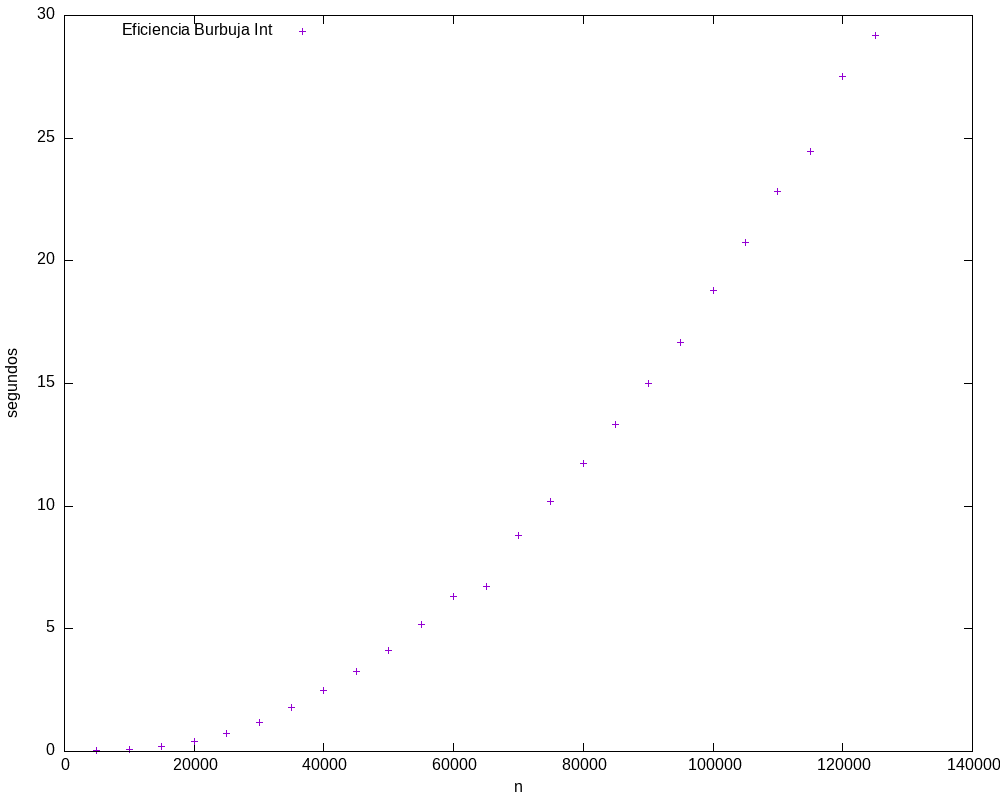
\includegraphics[width=0.8\linewidth]{images/Burbuja/graficos/int.png}
        \cprotect\caption{Tiempo de ejecución del algoritmo de Burbuja para \verb|int| en PC Irina.}
        \label{fig:Burbuja_int_graf}
    \end{figure}  
    \begin{figure}
        \centering
        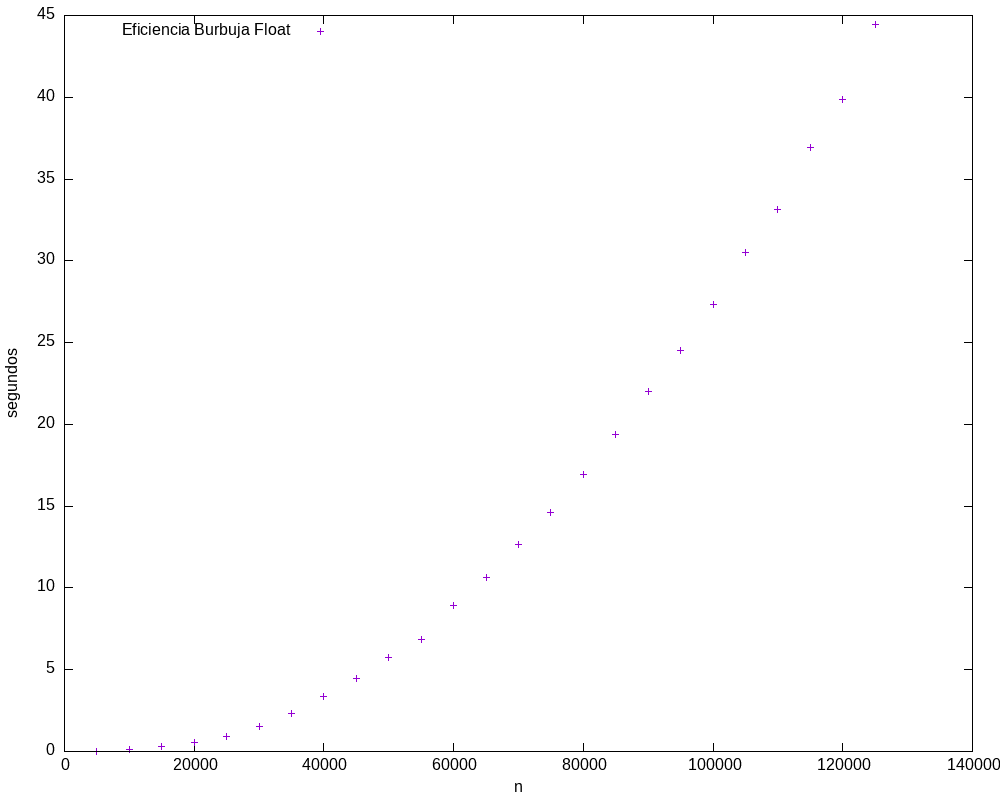
\includegraphics[width=0.8\linewidth]{images/Burbuja/graficos/float.png}
        \cprotect\caption{Tiempo de ejecución del algoritmo de Burbuja para \verb|float| en PC Irina.}
        \label{fig:Burbuja_float_graf}
    \end{figure}    
    \begin{figure}
        \centering
        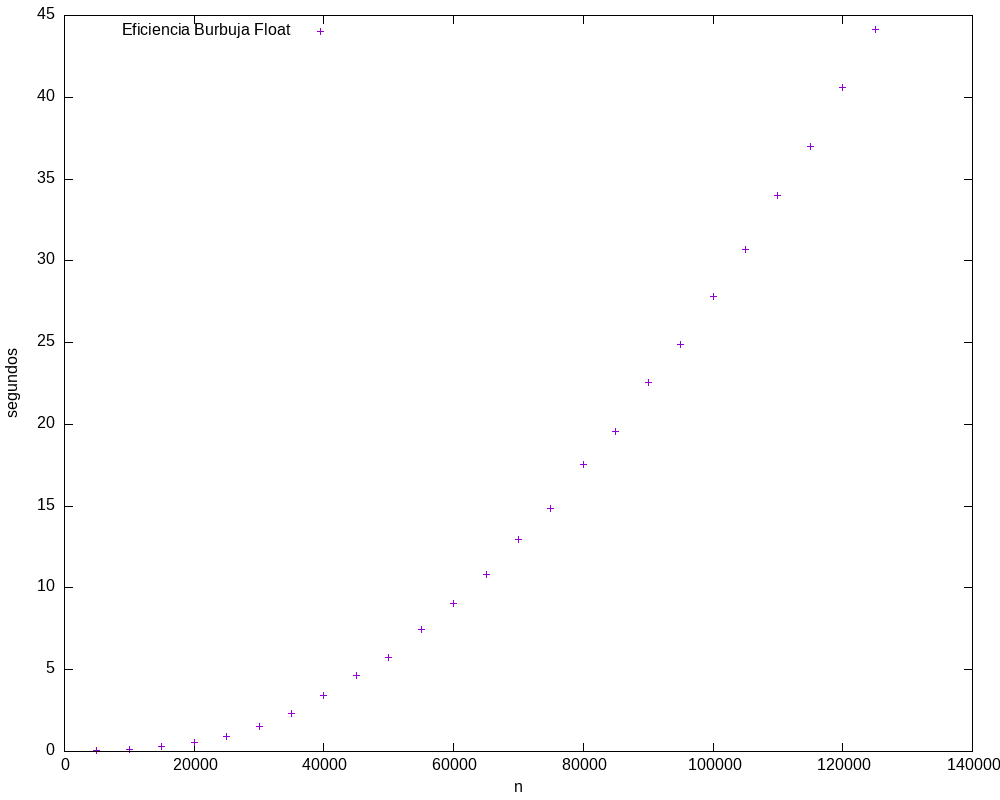
\includegraphics[width=0.8\linewidth]{images/Burbuja/graficos/double.png}
        \cprotect\caption{Tiempo de ejecución del algoritmo de Burbuja para \verb|double| en PC Irina.}
        \label{fig:Burbuja_double_graf}
    \end{figure}    
    \begin{figure}
        \centering
        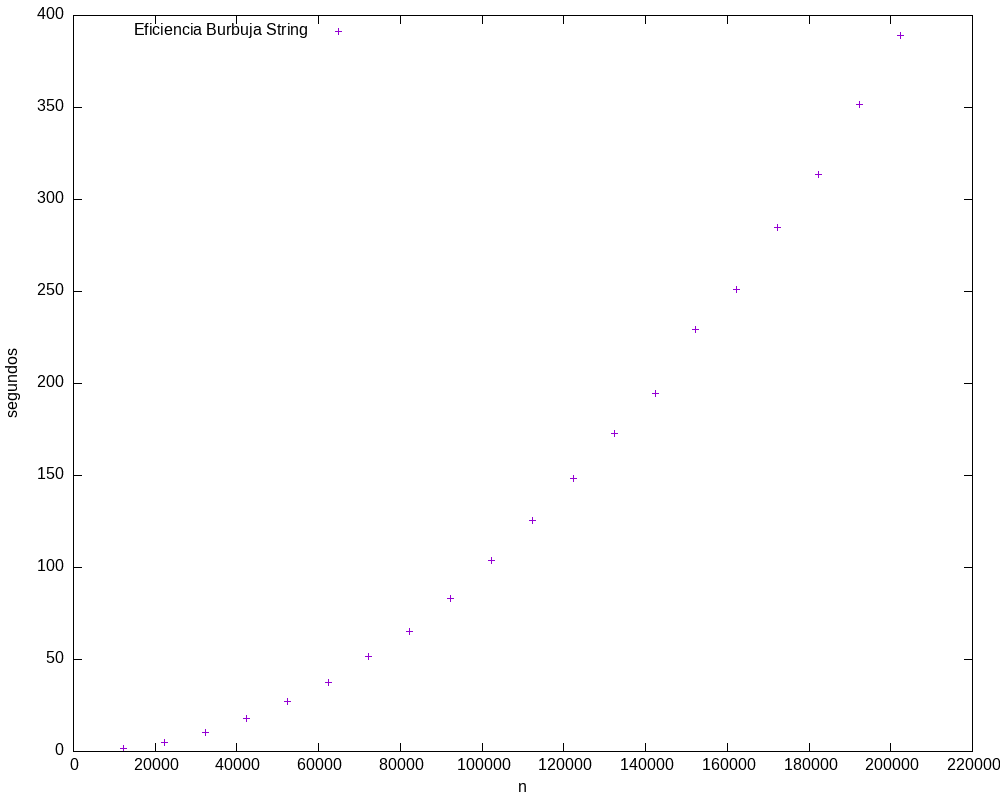
\includegraphics[width=0.8\linewidth]{images/Burbuja/graficos/str.png}
        \cprotect\caption{Tiempo de ejecución del algoritmo de Burbuja para \verb|string| en PC Irina.}
        \label{fig:Burbuja_string_graf}
    \end{figure}

    En las nubes de puntos de las Figuras \ref{fig:Burbuja_int_graf}, \ref{fig:Burbuja_float_graf}, \ref{fig:Burbuja_double_graf} y \ref{fig:Burbuja_string_graf} se observa bien el crecimiento cuadrático del algoritmo respecto a su entrada. También se nota cómo los tiempos dejan bastante que desear teniendo otros algoritmos mucho más rápidos para poder ordenar datos. No es recomendable, por lo tanto, usar burbuja en casi ninguna situación, e incluso en las que funciona ligeramente mejor es preferible usar el algoritmo de ordenación conocido como \verb|cocktail sort| (burbuja bidireccional), que mantiene el mejor caso de burbuja y se ejecuta mejor que este en el caso medio. En general, no hay un buen motivo para utilizar burbuja.
    
     \begin{figure}
        \centering
        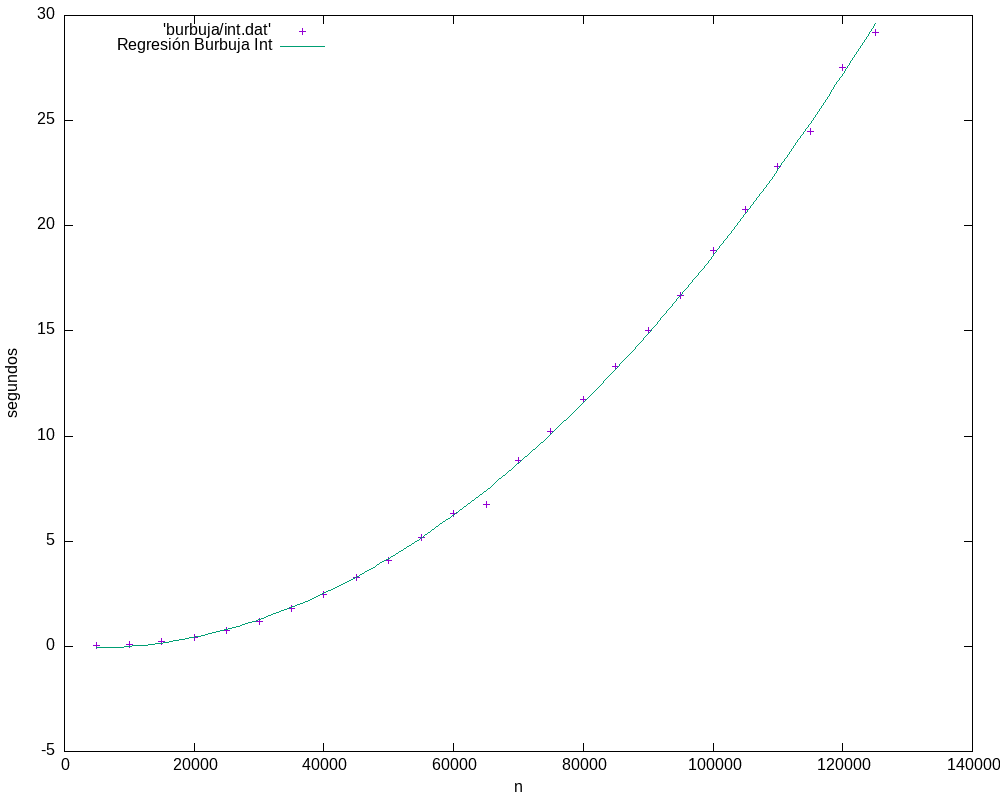
\includegraphics[width=0.8\linewidth]{images/Burbuja/graficos/ajusteInt.png}
        \cprotect\caption{Regresión del algoritmo de Burbuja para \verb|int| en PC Irina.}
        \label{fig:Burbuja_ajuste_int_graf}
    \end{figure}
    \begin{figure}
        \centering
        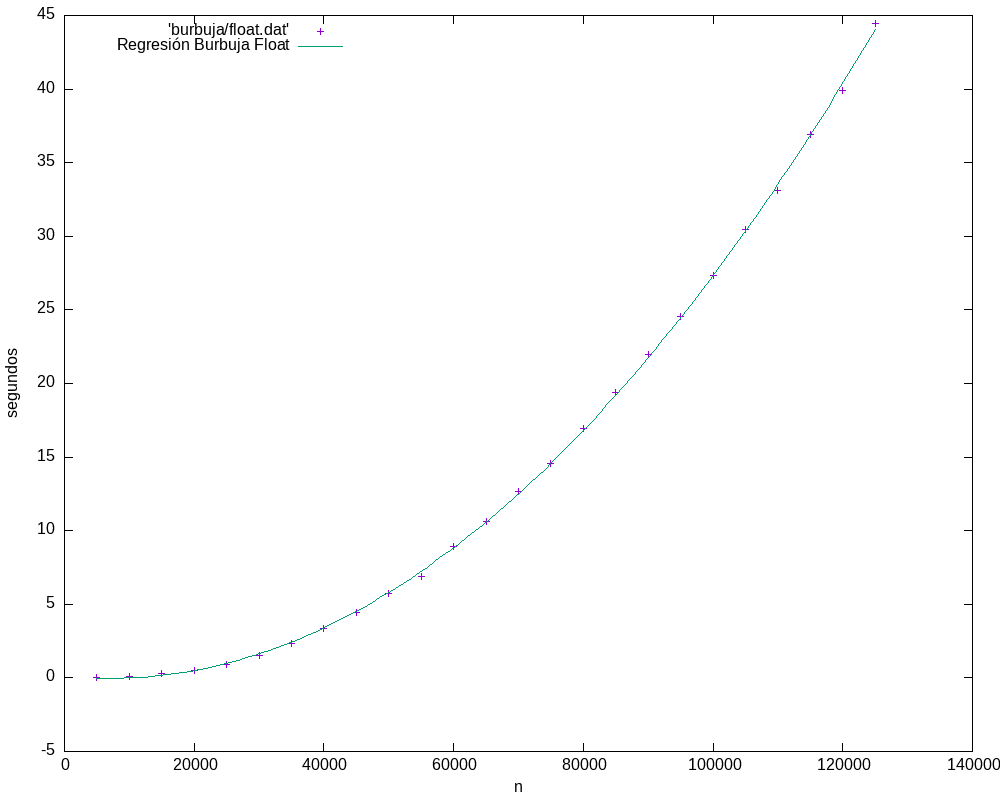
\includegraphics[width=0.8\linewidth]{images/Burbuja/graficos/ajusteFloat.png}
        \cprotect\caption{Regresión del algoritmo de Burbuja para \verb|float| en PC Inina.}
        \label{fig:Burbuja_ajuste_float_graf}
    \end{figure}
    \begin{figure}
        \centering
        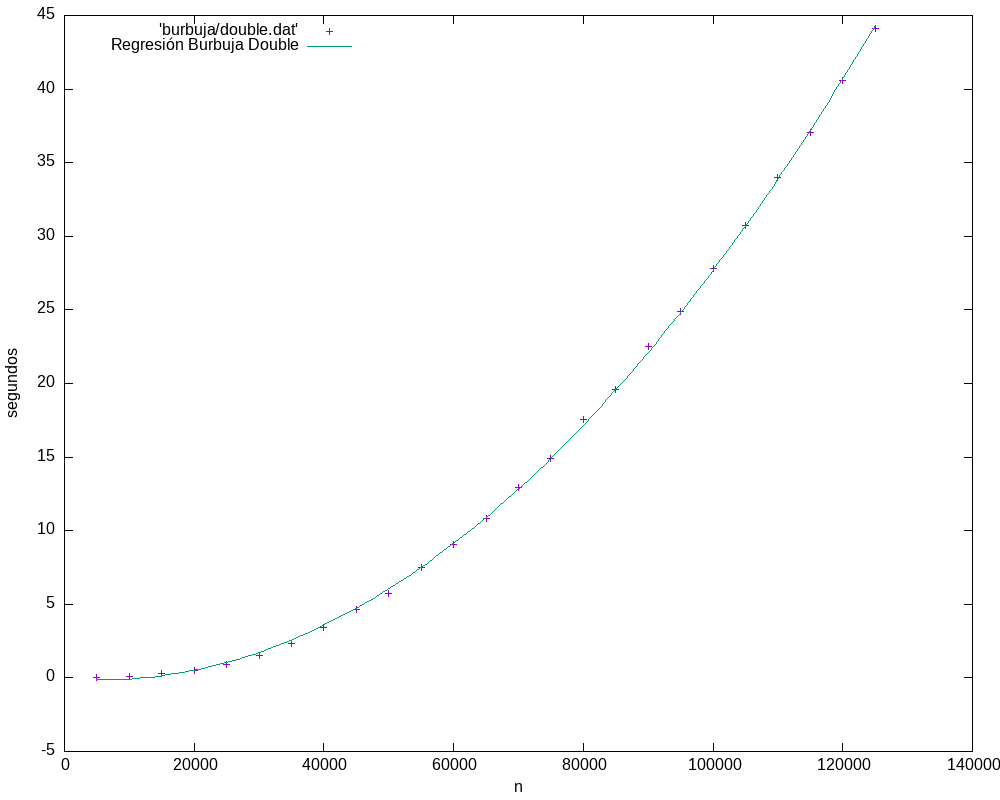
\includegraphics[width=0.8\linewidth]{images/Burbuja/graficos/ajusteDouble.png}
        \cprotect\caption{Regresión del algoritmo de Burbuja para \verb|double| en PC Irina.}
        \label{fig:Burbuja_ajuste_double_graf}
    \end{figure}
    \begin{figure}
        \centering
        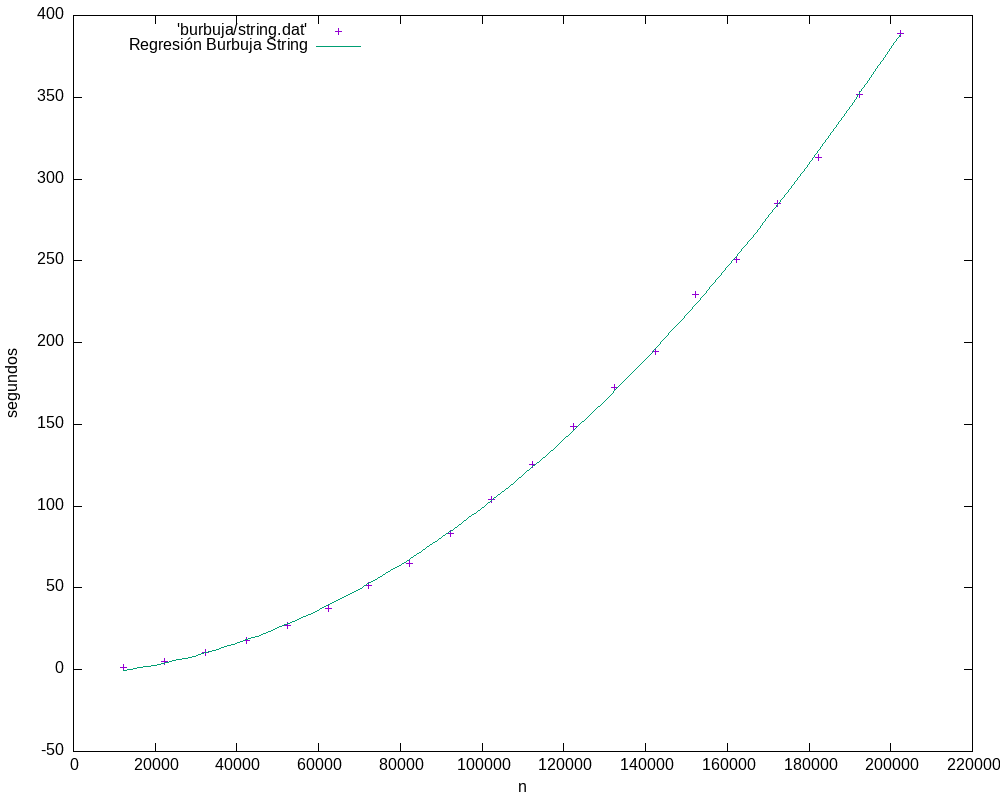
\includegraphics[width=0.8\linewidth]{images/Burbuja/graficos/ajusteString.png}
        \cprotect\caption{Regresión del algoritmo de Burbuja para \verb|string| en PC Irina.}
        \label{fig:Burbuja_ajuste_string_graf}
    \end{figure}

    
    \begin{itemize}
        \item Para \verb|ints|, se ha usado la función siguiente, que se observa en la Figura \ref{fig:Burbuja_ajuste_int_graf}:

        $$ f(x)= 2.03\cdot10^{-9} x^2 - 1.78\cdot10^{-6}x - 0.029$$
    
        \item Para \verb|float|, se ha usado la función siguiente, que se observa en la Figura \ref{fig:Burbuja_ajuste_float_graf}:

        $$ g(x)= 3.17\cdot10^{-9}x^2 -4.56\cdot10^{-5}x +0.14 $$
    
        \item Para \verb|double|, se ha usado la función siguiente, que se observa en la Figura \ref{fig:Burbuja_ajuste_double_graf}:
        
        $$ h(x)= 3.11\cdot10^{-9}x^2 -3.36\cdot10^{-5}x -0.0518 $$

        \item Para \verb|string|, se ha usado la función siguiente, que se observa en la Figura \ref{fig:Burbuja_ajuste_string_graf}:

        $$ s(x)= 8.94\cdot10^{-9}x^2 + 1.12\cdot10^{-4}x -3.22 $$
    \end{itemize}

    Estas regresiones nos indican cómo de bien podemos, con la nube de puntos dependiente de la entrada que elegimos, predecir el tiempo que tardaría una entrada de datos arbitraria en un caso medio. Cabe destacar que a pesar de que pueda ser mejor, para $n$ grande no va a ser mejor que el algoritmo de inserción, así que tampoco hay motivo para utilizar burbuja.

    Se aprecia muy bien en la Figura \ref{fig:Burbuja_Comparacion_graf} cómo el tipo de dato afecta a la velocidad con la que ordena el algoritmo de burbuja, como hemos justificado anteriormente con la tabla de valores del tiempo de ejecución según su entrada. Esta gráfica, sin embargo, en un ordenador con hardware dedicado al tratamiento de los tipos de coma flotante, se verían probablemente tres curvas juntas para los tipos \verb|int|, \verb|float| y \verb|double|, y una curva bastante alejada para los \verb|string|.
    \begin{figure}
        \centering
        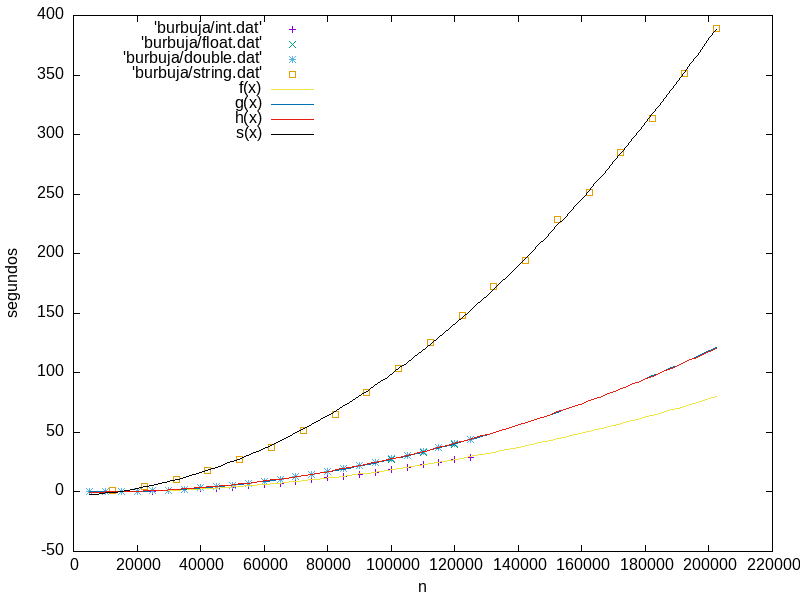
\includegraphics[width=0.8\linewidth]{images/Burbuja/graficos/BurbujaCompTipos.png}
        \cprotect\caption{Comparación de Burbuja para distintos tipos de datos en PC Irina.}
        \label{fig:Burbuja_Comparacion_graf}
    \end{figure}
    
    \textbf{Inserción}\\
    Hemos ejecutado el algoritmo de ordenación conocido por Inserción con una cantidad aleatorio creciente comenzando por 5000 datos y terminando en 125000 datos con saltos de 5000 para los tipos \verb|int|, \verb|float|, \verb|double|, \verb|string| siendo este último el más costoso; obteniendo la Tabla \ref{tab:Inserción_tiempos}, en la cual la primera columna hace referencia al número de datos usados y las siguientes cuatro sobre los tiempos de los distintos tipos. Sobre los datos de la Tabla \ref{tab:Inserción_tiempos} podemos observar las gráficas de las Figuras \ref{fig:Inserción_int_graf}, \ref{fig:Inserción_float_graf}, \ref{fig:Inserción_double_graf} y \ref{fig:Inserción_string_graf}.
    \begin{table}
        \centering
        \begin{tabular}{|l|l|l|l|l|}
            \hline
            $n$ & \verb|int| & \verb|float| & \verb|double| & \verb|string| \\
            \hline
            $5000$ & $0.0204147$ & $0.0204531$ & $0.0204161$ & $0.11739$ \\
            $10000$ & $0.0668181$ & $0.0706252$ & $0.0717277$ & $0.476915$ \\
            $15000$ & $0.150446$ & $0.15914$ & $0.162697$ & $1.03511$ \\
            $20000$ & $0.265347$ & $0.289009$ & $0.291386$ & $1.91591$ \\
            $25000$ & $0.422021$ & $0.452415$ & $0.465071$ & $3.02633$ \\
            $30000$ & $0.605959$ & $0.65003$ & $0.662947$ & $4.37451$ \\
            $35000$ & $0.826906$ & $0.891952$ & $0.900922$ & $5.88987$ \\
            $40000$ & $1.09136$ & $1.16696$ & $1.17208$ & $7.74376$ \\
            $45000$ & $1.40001$ & $1.48177$ & $1.4988$ & $9.79467$ \\
            $50000$ & $1.69897$ & $1.83223$ & $1.85276$ & $12.1064$ \\
            $55000$ & $2.06273$ & $2.21709$ & $2.24403$ & $15.5281$ \\
            $60000$ & $2.49409$ & $2.64314$ & $2.69843$ & $18.9615$ \\
            $65000$ & $2.89699$ & $3.14981$ & $3.12897$ & $21.8367$ \\
            $70000$ & $3.37379$ & $3.59713$ & $3.68795$ & $25.0129$ \\
            $75000$ & $3.86297$ & $4.23868$ & $4.26568$ & $29.1099$ \\
            $80000$ & $4.38083$ & $4.75756$ & $4.85197$ & $32.7821$ \\
            $85000$ & $5.01868$ & $5.47579$ & $5.74777$ & $36.8927$ \\
            $90000$ & $5.57376$ & $5.99755$ & $6.19353$ & $41.7275$ \\
            $95000$ & $6.29386$ & $6.82111$ & $6.91584$ & $46.0235$ \\
            $100000$ & $6.85596$ & $7.40268$ & $7.74474$ & $51.5689$ \\
            $105000$ & $7.89825$ & $8.44242$ & $8.62168$ & $56.5793$ \\
            $110000$ & $8.59807$ & $9.29984$ & $9.39702$ & $62.1997$ \\
            $115000$ & $9.60581$ & $10.0701$ & $10.2097$ & $67.7463$ \\
            $120000$ & $10.3022$ & $11.0502$ & $11.1417$ & $74.2626$ \\
            $125000$ & $11.0969$ & $11.9086$ & $12.0964$ & $77.8286$ \\
            \hline
        \end{tabular}
        \caption{Tiempos de ejecución para Inserción en el ordenador de Lucas.}
        \label{tab:Inserción_tiempos}
    \end{table}

    \begin{figure}
        \centering
        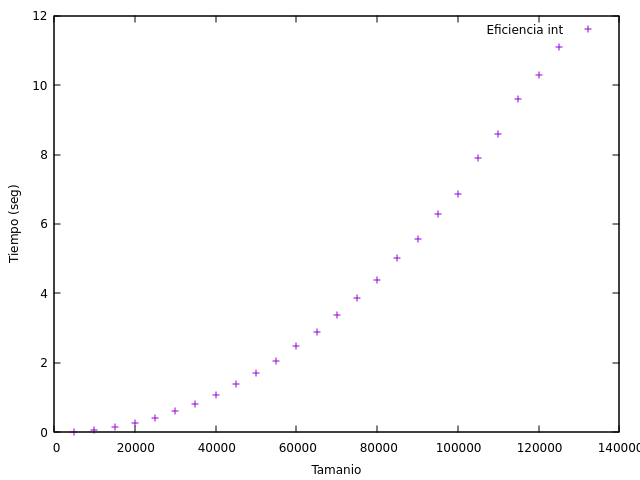
\includegraphics[width=0.8\linewidth]{images/Insercion/insercion_int_graf.png}
        \cprotect\caption{Tiempo de ejecución del algoritmo de Inserción para \verb|int| en PC Lucas.}
        \label{fig:Inserción_int_graf}
    \end{figure}
    \begin{figure}
        \centering
        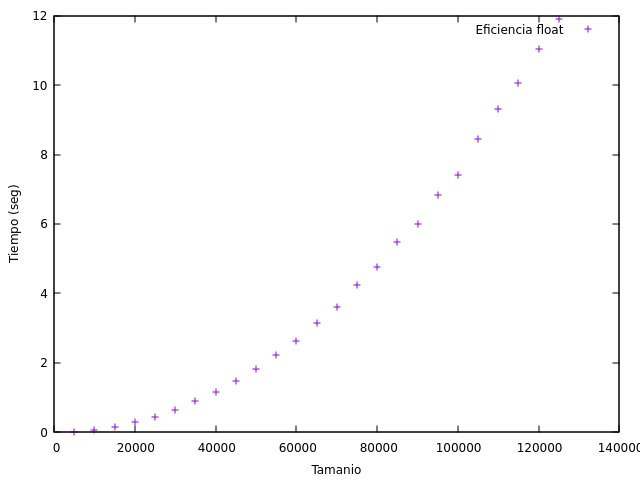
\includegraphics[width=0.8\linewidth]{images/Insercion/insercion_float_graf.png}
        \cprotect\caption{Tiempo de ejecución del algoritmo de Inserción para \verb|float| en PC Lucas.}
        \label{fig:Inserción_float_graf}
    \end{figure}
    \begin{figure}
        \centering
        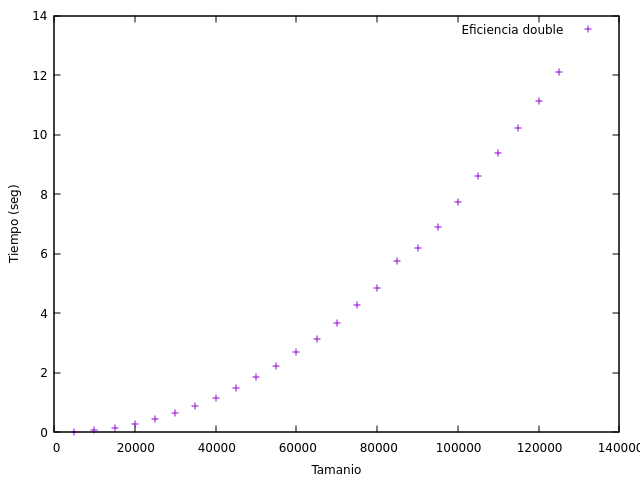
\includegraphics[width=0.8\linewidth]{images/Insercion/insercion_double_graf.png}
        \cprotect\caption{Tiempo de ejecución del algoritmo de Inserción para \verb|double| en PC Lucas.}
        \label{fig:Inserción_double_graf}
    \end{figure}
    \begin{figure}
        \centering
        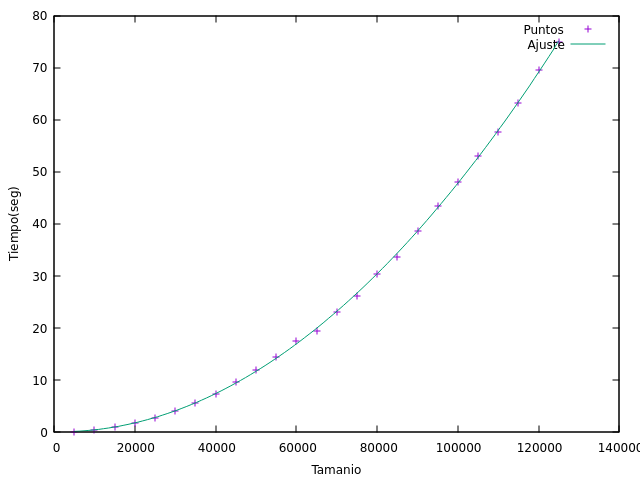
\includegraphics[width=0.8\linewidth]{images/Insercion/insercion_string_graf.png}
        \cprotect\caption{Tiempo de ejecución del algoritmo de Inserción para \verb|string| en PC Lucas.}
        \label{fig:Inserción_string_graf}
    \end{figure}

    Sobre los mismos datos de la Tabla \ref{tab:Inserción_tiempos} hemos realizado los siguientes ajustes, siendo todos cuadráticos:
    \begin{itemize}
        \item Para \verb|ints|, se ha usado la función siguiente, que se observa en la Figura \ref{fig:RegresionInsercionInt}:

        $$f(x)=7.58319\cdot10^{-10}-6.14623\cdot10^{-6}x+0.0843174x^2$$
    
        \item Para \verb|float|, se ha usado la función siguiente, que se observa en la Figura \ref{fig:RegresionInsercionFloat}:
    
        $$f(x)=7.98116\cdot10^{-10}-4.6311\cdot10^{-6}x+0.0548818x^2$$
    
        \item Para \verb|double|, se ha usado la función siguiente, que se observa en la Figura \ref{fig:RegresionInsercionDouble}:
    
        $$f(x)=8.00545\cdot10^{-10}-3.12454\cdot10^{-6}x+0.0218544x^2$$
    
        \item Para \verb|string|, se ha usado la función siguiente, que se observa en la Figura \ref{fig:RegresionInsercionString}:
    
        $$f(x)=5.00798\cdot10^{-9}-1.46519\cdot10^{-5}x-0.439829x^2$$
    \end{itemize}

    \begin{figure}
        \centering
        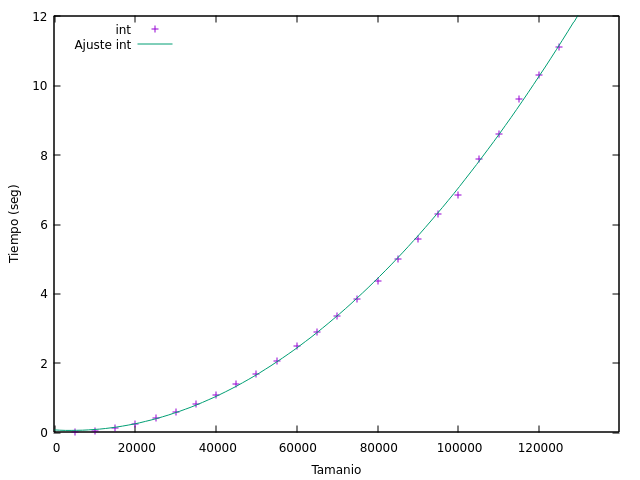
\includegraphics[width=0.8\linewidth]{images/Insercion/Ajuste int.png}
        \cprotect\caption{Regresión del algoritmo de Inserción para \verb|int| en el PC Lucas.}
        \label{fig:RegresionInsercionInt}
    \end{figure}

    \begin{figure}
        \centering
        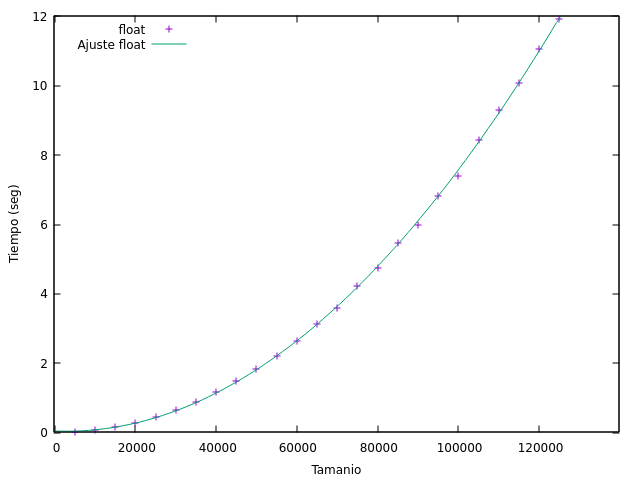
\includegraphics[width=0.8\linewidth]{images/Insercion/Ajuste float.png}
        \cprotect\caption{Regresión del algoritmo de Inserción para \verb|float| en el PC Lucas.}
        \label{fig:RegresionInsercionFloat}
    \end{figure}

    \begin{figure}
        \centering
        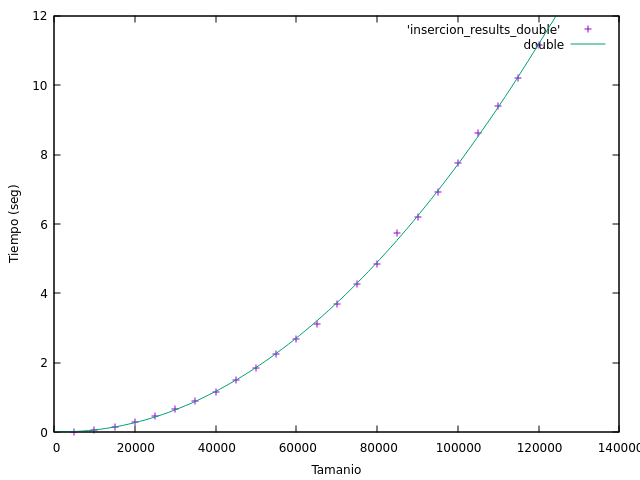
\includegraphics[width=0.8\linewidth]{images/Insercion/Ajuste double.png}
        \cprotect\caption{Regresión del algoritmo de Inserción para \verb|double| en el PC Lucas.}
        \label{fig:RegresionInsercionDouble}
    \end{figure}

    \begin{figure}
        \centering
        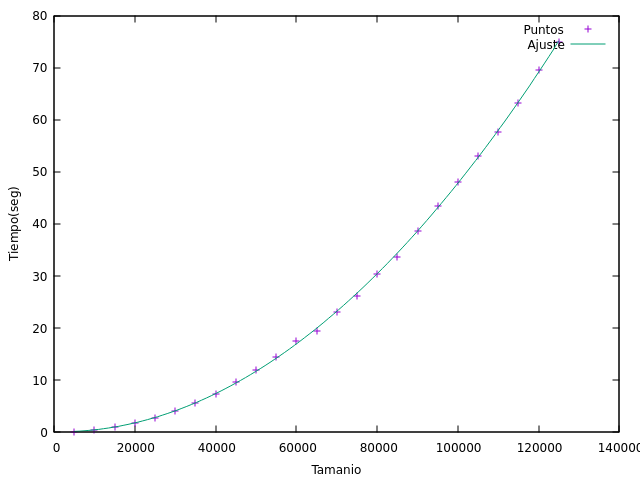
\includegraphics[width=0.8\linewidth]{images/Insercion/insercion_string_graf.png}
        \cprotect\caption{Regresión del algoritmo de Inserción para \verb|string| en el PC Lucas.}
        \label{fig:RegresionInsercionString}
    \end{figure}


    Por último, para concluir el estudio de la eficiencia empírica sobre este algoritmo de ordenación, en la Figura \ref{fig:ComparativaInsercionDatos} se han representado todos los tipos de datos para realizar una comparación de los mismos. Como ya se preveía, la ejecución de los tipos de dato \verb|string| son mucho más costosos de ordenar. De hecho este coste se percibe mucho debido a la cantidad de intercambios que se realiza durante la ordenación.  Por otro lado, los otros tipos no se distancian tanto entre sí; de hecho, es casi imperceptible. Esto es debido a que internamente los Bytes se mueven en una sola instrucción, en nuestro caso 8 Bytes (tamaño de línea de la caché), al tener un procesador de esta cantidad de Bytes. Más coloquialmente, se leen 64 bits siendo este el tamaño del \verb|double|; por tanto, independientemente del tipo de dato ya mencionado, siempre se realiza el movimiento en una instrucción.
    
    \begin{figure}
        \centering
        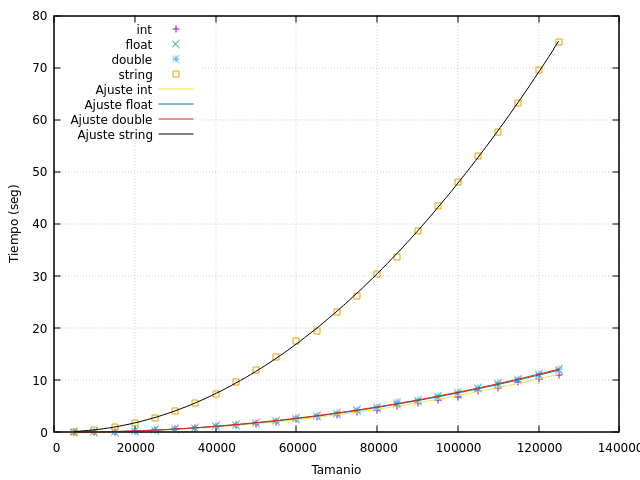
\includegraphics[width=0.8\linewidth]{images/Insercion/Comparacion_total_final.png}
        \caption{Comparativa de tipos de datos del algoritmo de Inserción en el PC Lucas.}
        \label{fig:ComparativaInsercionDatos}
    \end{figure}
    
    \subsubsection{Comparación de algoritmos cuadráticos}
    A continuación, vamos a comparar la ejecución del algoritmo de burbuja con el de Inserción para determinar qué algoritmo es más eficiente. Lo haremos tan solo con el tipo de dato \verb|int|, aunque se puede extrapolar al resto de tipos de datos. En la Tabla \ref{tab:comp_cuadraticos} se encuentran los datos de ambos algoritmos, representados en la Figura \ref{fig:comp_cuadraticos}.
    \begin{table}
        \centering
        \begin{tabular}{|l|l|l|}
            \hline
            $n$ & Burbuja & Inserción \\
            \hline
            $5000$ & $0.0320169$ & $0.0315755$ \\
            $10000$ & $0.121503$ & $0.0695729$ \\
            $15000$ & $0.318309$ & $0.154259$ \\
            $20000$ & $0.655574$ & $0.271925$ \\
            $25000$ & $1.14731$ & $0.430184$ \\
            $30000$ & $1.6936$ & $0.619942$ \\
            $35000$ & $2.38803$ & $0.858703$ \\
            $40000$ & $3.10454$ & $1.1165$ \\
            $45000$ & $4.14383$ & $1.40402$ \\
            $50000$ & $5.05033$ & $1.72773$ \\
            $55000$ & $6.29143$ & $2.11243$ \\
            $60000$ & $7.41145$ & $2.50072$ \\
            $65000$ & $9.05342$ & $2.95596$ \\
            $70000$ & $10.2067$ & $3.46206$ \\
            $75000$ & $11.9712$ & $3.98734$ \\
            $80000$ & $13.453$ & $4.48404$ \\
            $85000$ & $15.48$ & $5.08662$ \\
            $90000$ & $17.3659$ & $5.71736$ \\
            $95000$ & $19.1808$ & $6.43874$ \\
            $100000$ & $21.7095$ & $7.0535$ \\
            $105000$ & $24.2073$ & $8.00074$ \\
            $110000$ & $26.3358$ & $8.80258$ \\
            $115000$ & $29.268$ & $9.68143$ \\
            $120000$ & $31.244$ & $10.3124$ \\
            $125000$ & $34.563$ & $11.236$ \\
            \hline
        \end{tabular}
        \cprotect\caption{Tiempos de Burbuja para \verb|int| con Inserción, ambos en PC Lucas.}
        \label{tab:comp_cuadraticos}
    \end{table}
    \begin{figure}
        \centering
        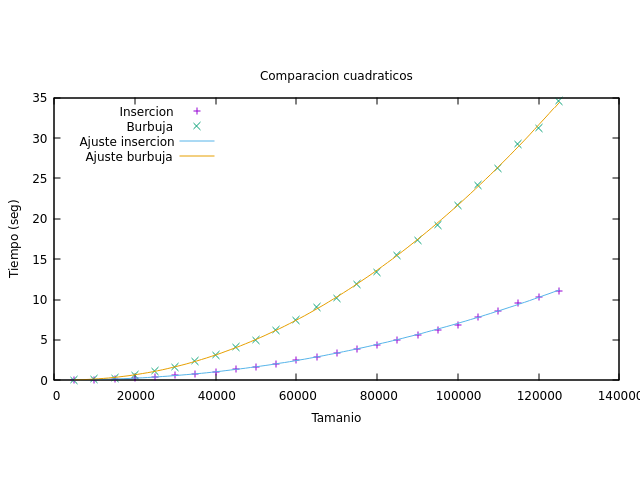
\includegraphics[width=0.85\linewidth]{images/Comparaciones/Comparacion_cuadraticos.png}
        \cprotect\caption{Comparación de Burbuja con Inserción para \verb|int|, ambos en PC Lucas.}
        \label{fig:comp_cuadraticos}
    \end{figure}

    Es fácil de intuir que el algoritmo de ordenación conocido como Burbuja ha presentado peor eficiencia que el algoritmo de Inserción. En gran medida, esto es debido a que en el primero de ellos se realizan un mayor número de intercambios. Por tanto, esta es la razón fundamental por la cual este algoritmo es menos eficiente que el segundo de ellos. 

    Además, cabe destacar que, aunque ambos sean cuadráticos, esto no quiere decir que tengan el mismo tiempo de ejecución en todos los ámbitos. Asimismo, se puede resaltar la gran diferencia que hay entre ellos a medida que va aumentando el número de datos. Si nos fijamos, el algoritmo de Inserción tiene un crecimiento mucho menos pronunciado que el algoritmo Burbuja; el cual con $125000$ datos tiene tiempo de ejecución de $35$ segundos. 

    En conclusión, el algoritmo de Inserción es más eficiente que el algoritmo Burbuja. No obstante, ambos tiene un orden de eficiencia cuadrático diferenciándose en las constantes. Esto último nos da a entender que las constantes también tienen un significado importante en el estudio de la eficiencia de algoritmos.


    \subsubsection{Comparación en distinto hardware}
    Hemos elegido el algoritmo de Inserción como candidato de algoritmo cuadrático a ejecutarse en todos los ordenadores usando el tipo de dato \verb|int| (se extrapola al resto de tipos de datos). A continuación, en la Tabla \ref{tab:comp_hardware_insercion} mostramos los tiempos de ejecución en cada uno de los ordenadores, así como la gráfica de la Figura \ref{fig:CompHardwareInsercion}, que nos muestra estos tiempos visualmente.
    \begin{table}
        \centering
        \begin{tabular}{|l|l|l|l|l|l|}
            \hline
            $n$ & José Juan & Arturo & Irina & Lucas & Airam \\
            \hline
            $5000$ & $0.0215686$ & $0.0405246$ & $0.014567$ & $0.0315755$ & $0.0516634$ \\
            $10000$ & $0.0867437$ & $0.122055$ & $0.0629751$ & $0.0695729$ & $0.196678$ \\
            $15000$ & $0.195987$ & $0.26581$ & $0.139884$ & $0.154259$ & $0.429474$ \\
            $20000$ & $0.345769$ & $0.478241$ & $0.255842$ & $0.271925$ & $0.75662$ \\
            $25000$ & $0.534336$ & $0.747736$ & $0.404021$ & $0.430184$ & $1.18137$ \\
            $30000$ & $0.779653$ & $1.06181$ & $0.555394$ & $0.619942$ & $1.69171$ \\
            $35000$ & $1.05228$ & $1.45304$ & $0.712199$ & $0.858703$ & $2.30821$ \\
            $40000$ & $1.3656$ & $1.91375$ & \underline{$0.973901$} & $1.1165$ & \underline{$2.98189$} \\
            $45000$ & $1.74368$ & $2.41838$ & $1.21816$ & $1.40402$ & $3.79044$ \\
            $50000$ & $2.14439$ & $2.96104$ & $1.58308$ & $1.72773$ & $4.77736$ \\
            $55000$ & $2.62142$ & $3.58726$ & $1.90068$ & $2.11243$ & $5.66737$ \\
            $60000$ & $3.11232$ & $4.26268$ & $2.27818$ & $2.50072$ & $6.81823$ \\
            $65000$ & $3.61466$ & $5.01638$ & $2.64389$ & $2.95596$ & $7.95222$ \\
            $70000$ & $4.20397$ & $5.79249$ & $2.9987$ & $3.46206$ & $9.38579$ \\
            $75000$ & $4.82346$ & $6.69775$ & $3.54469$ & $3.98734$ & $10.6808$ \\
            $80000$ & $5.50419$ & $7.67351$ & $4.05363$ & $4.48404$ & $11.9706$ \\
            $85000$ & $6.1988$ & $8.55686$ & $4.63762$ & $5.08662$ & $13.7397$ \\
            $90000$ & $6.94836$ & $9.61363$ & $5.14756$ & $5.71736$ & $15.2493$ \\
            $95000$ & $7.76365$ & $10.7204$ & $5.75839$ & $6.43874$ & $17.0127$ \\
            $100000$ & $8.56124$ & $11.8724$ & $6.33938$ & $7.0535$ & $18.7912$ \\
            $105000$ & $9.5075$ & $13.0696$ & $7.08369$ & $8.00074$ & $20.7604$ \\
            $110000$ & $10.3898$ & $14.3768$ & $7.66268$ & $8.80258$ & $22.642$ \\
            $115000$ & $11.3695$ & $15.6251$ & $8.4614$ & $9.68143$ & $24.894$ \\
            $120000$ & $12.314$ & $17.2278$ & $9.19415$ & $10.3124$ & $27.0555$ \\
            $125000$ & $13.4283$ & $18.6903$ & \underline{$10.1265$} & $11.236$ & \underline{$29.3985$} \\
            \hline
        \end{tabular}
        \cprotect\caption{Comparación de Inserción en distinto hardware para \verb|int|.}
        \label{tab:comp_hardware_insercion}
    \end{table}
    \begin{figure}
        \centering
        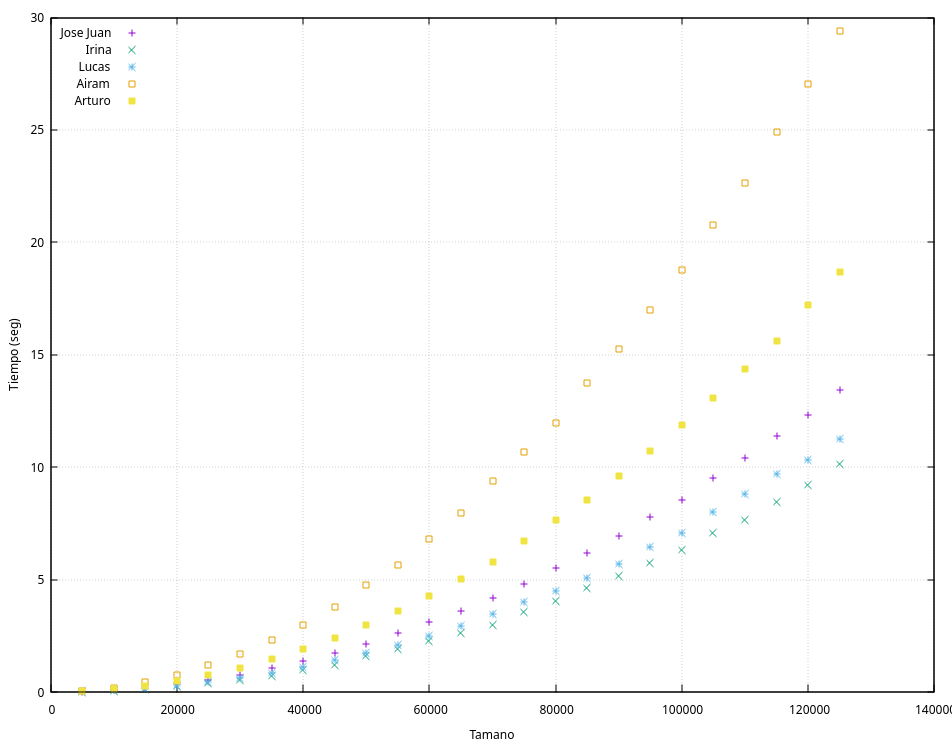
\includegraphics[width=0.8\linewidth]{images/Comparaciones_hardware/Comparacion_hardware_insercion.png}
        \cprotect\caption{Algoritmo de Inserción en todos los PCs para datos de tipo \verb|int|.}
        \label{fig:CompHardwareInsercion}
    \end{figure}

    En esta, podemos ver de forma muy clara el comportamiento de un algoritmo cuadrático en distinto hardware (con burbuja, el resultado habría sido similar). Podemos observar que para valores no muy grandes de $n$ como $40000$, obtenemos una diferencia de $2$ segundos en cuanto a tiempo de ejecución, que al principio no parece una diferencia muy grande. Sin embargo, a medida que aumentamos el tamaño de $n$, observamos cómo el crecimiento de la pendiente varía considerablemente en distinto hardware: PCs como el de Irina, Lucas o José Juan no presentan un crecimiento muy grande de la pendiente para los tamaños considerados; el PC de Arturo presenta un crecimiento moderado y el de Airam un crecimiento bastante grande. Esta variación de crecimiento, por la naturaleza de la función cuadrática, es bastante notorio ya para valores de $n$ más grandes, como el último valor de $n$ que consideramos, $125000$, ya podemos observar una gran diferencia en tiempos de ejecución, de hasta $20$ segundos respecto al hardware con mejores resultados (el PC de Irina) y el hardware con peores resultados (el PC de Airam). Esto nos lleva a pensar que el tiempo de ejecución en cuanto a algoritmos cuadráticos depende bastante del hardware que elijamos para tamaños del problema suficientemente grandes, pero cabe destacar que el ordenador de Airam parece tener un fallo que impide que se aprovechen bien sus prestaciones.
    
    \subsection{Algoritmos linear-logarítmicos}
    \subsubsection{Análisis teórico}
    \textbf{Mergesort}
    
    El algoritmo se encuentra disponible en el Código Fuente \ref{code:Mergesort}.
    %uwu
    \begin{listing}
        \begin{minted}[linenos,xleftmargin=2cm]{c++}
void fusion(int T[], int inicial, int final, int U[], int V[]){
    int j = 0;
    int k = 0;

    for(int i = inicial; i < final; i++)
        if(U[j] < V[k]){
            T[i] = U[j];
            j++;
        }else{
            T[i] = V[k];
            k++;
        }
}

void mergesort(int T[], int inicial, int final){
    if (final - inicial < UMBRALMS)
        burbuja(T, inicial, final);
    else{
        int k = (final - inicial)/2;
        int *U = new int[k - inicial + 1];
        assert(U==0);
        int l, l2;

        for(l = 0, l2 = inicial; l<k-inicial; l++, l2++)
            U[l] = T[l2];
        U[l] = INT_MAX;

        int *V = new int[final - k + 1];
        assert(V == 0);
        for(l = 0, l2 = k; l < final - k; l++, l2++)
            V[l] = T[l2];

        V[l] = INT_MAX;
        mergesort(U, 0, k-inicial);
        mergesort(V, 0, final - k);
        fusion(T, inicial, final, U, V);
        delete[] U;
        delete[] V;
    }
}
    \end{minted}
    \caption{Ordenación mediante el método de Mergesort.}
    \label{code:Mergesort}
    \end{listing}

    Para el análisis teórico, comenzamos definiendo el tamaño de nuestro problema, $n$. Tendremos que \verb|final| será $n$ y que \verb|inicial| será $0$. Primero, analizamos el tiempo de ejecución de la función \verb|fusion|. El bucle ejecuta las líneas 6 a 12 que se ejecutan en un tiempo constante, llamémosle $a$. Por tanto, el tiempo de ejecución vendrá dado por
    $$\sum_{i=0}^{n-1} a = a\cdot n$$
    que claramente es de orden $O(n)$. A continuación, analizamos la función Mergesort. Suponemos que entramos por la rama del \verb|else|, ya que buscamos comportamientos asintóticos $(n\ggg)$. Podemos acotar la secuencia de instrucciones de las líneas 19 a 22 por una constante $b$. El bucle de la línea 24 se ejecuta un total de $\frac{n}{2}$ veces y su cuerpo es de orden constante, luego podemos asumir una eficiencia de $\frac{n}{2}$. El mismo razonamiento se aplica a las líneas 26 a 29, pueden ser acotadas por una constante, y ahora el bucle de la línea 30 también tiene eficiencia $\frac{n}{2}$. A continuación, se realizan dos llamadas a la misma función, luego si la función tiene un tiempo de ejecución $T(n)$, asumimos que las líneas 34 y 35 tendrán uno de $T\left(\nicefrac{n}{2}\right)$. Finalmente, la línea 36 tiene una eficiencia de $O(n)$. Resumiendo, la parte del \verb|else| tiene una eficiencia total de:
    $$T(n) = 2T\left(\dfrac{n}{2}\right)+n$$
    Ahora, analizamos la parte del \verb|if|. Esta llama a la función \verb|burbuja|, que sabemos que es de orden $O(n^2)$. Por tanto, la recurrencia es:
    $$T(n) = \left\{\begin{array}{lcl}
        2T\left(\dfrac{n}{2}\right)+n & si & n \geq \verb|UMBRALMS| \\
        n^2 & si & n < \verb|UMBRALMS|
    \end{array} \right.$$
    Haciendo en la primera ecuación el cambio de variable $n = 2^m$:
    $$T(2^m) = 2T(2^{m-1})+2^m \qquad \text{ si } m \geq \log_2(\verb|UMBRALMS|)$$
    Renombrando $t_m = T(2^m)$, tenemos:
    $$t_m - 2t_{m-1} = 2^m$$
    La ecuación característica asociada a la parte homogénea, con $t_m=x^m$, es:
    $$x^m-2x^{m-1}=x^{m-1}(x-2)=0$$
    Como $x^m> 0$ para todo $m\in \bb{N}$, tenemos que la única solución de la ecuación característica es $x=2$, con multiplicidad simple. Respecto a la parte no homogénea, tenemos que $2^m=2^m(m^0)$, por lo que el polinomio característico de la ecuación en diferencias queda:
    \begin{equation*}
        p(x)=(x-2)(x-2)=(x-2)^2
    \end{equation*}
    Por tanto, la solución general de la ecuación en diferencias será de la forma:
    $$t_m = c_1 \cdot 2^m + c_2 \cdot m \cdot 2^m \qquad c_2,c_2\in \bb{R}$$
    Deshaciendo el cambio de variable, $m=\log_2 n$, tenemos que:
    $$T(n) = c_1\cdot 2^{\log_2 n}  +c_2\cdot \log_2 n \cdot 2^{\log_2 n}
    =
    c_1 \cdot n + c_2 \cdot n \log_2(n)\in O(n\log n)$$
    Por tanto, se tiene que $T(n) \in O(n\log n)$.\\

    \textbf{Quicksort}

    El código del algoritmo se encuentra en Código fuente \ref{code:quicksort}.
    
    \begin{listing}
        \begin{minted}[linenos,xleftmargin=2cm]{c++}
void quicksort(int T[], int inicial, int final){
    int k;
    if (final - inicial < UMBRAL_QS){
        insercion(T, inicial, final);
    } else{
        dividir_qs(T, inicial, final, k);
        quicksort(T, inicial, k);
        quicksort(T, k+1, final);
    }
}
void dividir_qs(int T[], int inicial, int final, int & pp)
{
  int pivote, aux;
  int k, l;

  pivote = T[inicial];
  k = inicial;
  l = final;
  do {
    k++;
  } while (k < final-1)) && ((T[k] <= pivote);
  do {
    l--;
  } while (T[l] > pivote);
  while (k < l) {
    aux = T[k];
    T[k] = T[l];
    T[l] = aux;
    do k++; while (T[k] <= pivote);
    do l--; while (T[l] > pivote);
  };
  aux = T[inicial];
  T[inicial] = T[l];
  T[l] = aux;
  pp = l;
};

        \end{minted}
        \caption{Algoritmo de ordenación por el método de Quicksort.}
        \label{code:quicksort}
    \end{listing}
    Comenzamos definiendo el tamaño del problema, teniendo que \verb|final| será $n$ y que \verb|inicial| será $0$. Estudiamos en primer lugar la eficiencia de la función \verb|dividir_qs|. Tenemos que las líneas 13 a 18 no dependen de $n$, por lo son de orden $O(1)$; al igual que las líneas 32 a 35. Las líneas 19 a 31 describen dos índices, \verb|l| y \verb|k|, que se desplazan desde los dos extremos hasta encontrarse. Por tanto, siempre se encontrarán tras $n$ iteraciones, por lo que esta parte es de orden $O(n)$. Por tanto, de forma general, podemos decir que la función \verb|dividir_qs| es de orden $O(n)$.
    

    Estudiamos ahora la eficiencia de la función \verb|Quicksort|. La línea 2 es despreciable, ya que es de tiempo constante. En el caso de que se tome la rama del \verb|if|, tenemos que se usa el algoritmo de Inserción, que es $O(n^2)$. En el caso del \verb|else|, se ejecuta la función \verb|dividir_qs|, que es de orden $O(n)$, y dos llamadas recursivas. No obstante, la eficiencia del algoritmo Quicksort depende de la elección del pivote. Distinguimos:
    \begin{description}
        \item[Caso peor.] Supongamos que el vector original se divide en uno de tamaño $1$ y en otro de tamaño $n-1$ en todas las iteraciones; algo que ocurrirá si los elementos están repetidos, ordenados o casi ordenados. Tenemos que:
        \begin{equation*}
            T(n) = \left\{
            \begin{array}{ccc}
                n^2 & \text{si} & n< \verb|UMBRAL_QS|\\
                T(n-1) + T(1) + c_2n +c_3' & \text{si} & n\geq \verb|UMBRAL_QS|
            \end{array}
            \right.
        \end{equation*}

        Como $T(1)$ es para un valor de $n$ fijo, tenemos que se puede acotar por una constante, por lo que:
        \begin{equation*}
            T(n) = \left\{
            \begin{array}{ccc}
                n^2 & \text{si} & n< \verb|UMBRAL_QS|\\
                T(n-1) + c_2n +c_3 & \text{si} & n\geq \verb|UMBRAL_QS|
            \end{array}
            \right.
        \end{equation*}

        Aplicando el cambio de variable $T(n)=x^n$, la parte homogénea queda:
        \begin{equation*}
            x^n - x^{n-1} = 0 \Longrightarrow
            x^{n-1}(x-1)=0
        \end{equation*}

        Por tanto, la única solución es $x=1$, con multiplicidad simple. Respecto a la parte no homogénea, tenemos que $c_2n+c_3=1^n(c_2n^1 + c_3n^0)$, por lo que el polinomio característico de la Ley de Recurrencia queda:
        \begin{equation*}
            p(x)=(x-1)(x-1)^2 = (x-1)^3
        \end{equation*}

        Por tanto, la solución a la Ley de Recurrencia es:
        \begin{equation*}
            T(n)=x^n = k_1 + k_2n + k_3n^2 \in O(n^2)
        \end{equation*}

        \item[Caso mejor.] Supongamos que en cada división se parte el vector en dos problemas de tamaño igual, teniendo entonces que:
        \begin{equation*}
            T(n) = \left\{
            \begin{array}{ccc}
                n^2 & \text{si} & n< \verb|UMBRAL_QS|\\
                2T\left(\dfrac{n}{2}\right) + c_2n +c_3 & \text{si} & n\geq \verb|UMBRAL_QS|
            \end{array}
            \right.
        \end{equation*}

        Aplicamos en primer lugar el cambio de variable $n=2^m$, quedándonos:
        \begin{equation*}
            T(2^m) = \left\{
            \begin{array}{ccc}
                4^m & \text{si} & m< \log_2\verb|UMBRAL_QS|\\
                2T\left(2^{m-1}\right) + c_2\cdot 2^m +c_3 & \text{si} & m\geq \log_2 \verb|UMBRAL_QS|
            \end{array}
            \right.
        \end{equation*}

        Expresando $T(2^m)=x^m$, tenemos que la parte homogénea queda:
        \begin{equation*}
            x^m - 2x^{m-1} = 0 \Longrightarrow
            x^{m-1}(x-2)=0
        \end{equation*}

        Por tanto, la única solución es $x=2$, con multiplicidad simple. Respecto a la parte no homogénea, tenemos que $c_2\cdot 2^m+c_3=2^m (c_2n^0)+1^m(c_3n^0)$, por lo que el polinomio característico de la Ley de Recurrencia queda:
        \begin{equation*}
            p(x)=(x-2)(x-2)(x-1) = (x-2)^2(x-1)
        \end{equation*}

        Por tanto, la solución a la Ley de Recurrencia es:
        \begin{equation*}
            T(2^m)=x^m = k_1 + k_2\cdot 2^m + k_3\cdot m2^m
        \end{equation*}

        Deshaciendo el cambio de variable $m=\log_2 n$, tenemos que:
        \begin{equation*}
            T(n)=k_1 + k_2\cdot n + k_3 \log_2n \cdot n
            \in O(n\log n)
        \end{equation*}
    \end{description}

    Tenemos entonces que la eficiencia del algoritmo Quicksort es compleja de calcular, ya que depende de la elección del elemento de pivote. Como cualquier algoritmo de ordenación basado en la técnica \emph{``divide y vencerás''}, es necesario que esa división no se haga de una forma excesivamente desequilibrada, para que el tamaño de los dos nuevos subproblemas sea más pequeño.
    
    \subsubsection{Análisis empírico e híbrido}
    \textbf{Mergesort}

    Hemos ejecutado el algoritmo de ordenación conocido por Mergesort con una cantidad aleatoria creciente comenzando en $50000$ hasta $1250000$ con saltos de $50000$ para los tipos de datos \verb|int|, \verb|double|, \verb|float|; y tamaños desde $12308$ hasta $202308$ con saltos de $10000$ para \verb|string|, siendo este último el más costoso; obteniendo la Tabla \ref{tab:Mergesort_tiempos}.
    \begin{table}
        \centering
        \begin{tabular}{|l|l|l|l||l||l|l|}
             \hline
            $n$ & \verb|int| & \verb|double| & \verb|float| &\qquad\qquad& $n$ & \verb|string| \\
             \hline
            $50000$ & $0.014839$& $0.017539$& $0.014244$&&$12308$ & $0.026039$ \\
            $100000$ & $0.025333$& $0.033689$& $0.0279$&&$22308$ & $0.034568$ \\
            $150000$ & $0.038744$& $0.048785$& $0.037897$&&$32308$ & $0.042481$ \\
            $200000$ & $0.051856$& $0.06467$& $0.055116$&&$42308$ & $0.060849$ \\
            $250000$ & $0.056825$& $0.077173$& $0.061077$&&$52308$ & $0.060711$ \\
            $300000$ & $0.083605$& $0.091396$& $0.09201$&&$62308$ & $0.080397$ \\
            $350000$ & $0.107423$& $0.107569$& $0.124285$&&$72308$ & $0.105116$ \\
            $400000$ & $0.11874$& $0.14035$& $0.124493$&&$82308$ & $0.120913$ \\
            $450000$ & $0.124092$& $0.136582$& $0.131188$&&$92308$ & $0.17803$ \\
            $500000$ & $0.134394$& $0.150366$& $0.138771$&&$102308$ & $0.128233$ \\
            $550000$ & $0.15722$& $0.17314$& $0.163911$&&$112308$ & $0.142492$ \\
            $600000$ & $0.168724$& $0.176033$& $0.180171$&&$122308$ & $0.157295$ \\
            $650000$ & $0.172775$& $0.2104$& $0.189866$&&$132308$ & $0.180138$ \\
            $700000$ & $0.209681$& $0.230459$& $0.219616$&&$142308$ & $0.198765$ \\
            $750000$ & $0.234851$& $0.254745$& $0.247467$&&$152308$ & $0.219851$ \\
            $800000$ & $0.250391$& $0.25588$& $0.268727$&&$162308$ & $0.243553$ \\
            $850000$ & $0.211862$& $0.227545$& $0.248201$&&$172308$ & $0.273034$ \\
            $900000$ & $0.222096$& $0.244035$& $0.2348$&&$182308$ & $0.322363$ \\
            $950000$ & $0.24649$& $0.263679$& $0.250608$&&$192308$ & $0.317648$ \\
            $1000000$ & $0.315176$& $0.27787$& $0.273616$&&$202308$ & $0.344353$ \\
            $1050000$ & $0.278162$& $0.29704$& $0.285182$ & & & \\
            $1100000$ & $0.284839$& $0.314768$& $0.307615$ & & & \\
            $1150000$ & $0.303776$& $0.337459$& $0.323439$ & & & \\
            $1200000$ & $0.31913$& $0.351971$& $0.343243$ & & & \\
            $1250000$ & $0.34263$& $0.376201$& $0.361719$ & & & \\
             \hline
        \end{tabular}
        \caption{Tiempos de ejecución para Mergesort en el ordenador de Arturo.}
        \label{tab:Mergesort_tiempos}
    \end{table}

    Sobre los datos de la Tabla \ref{tab:Mergesort_tiempos} podemos observar las gráficas de las Figuras \ref{fig:Mergesort_int_graf}, \ref{fig:Mergesort_float_graf}, \ref{fig:Mergesort_double_graf} y \ref{fig:Mergesort_string_graf}.

    \begin{figure}
        \centering
        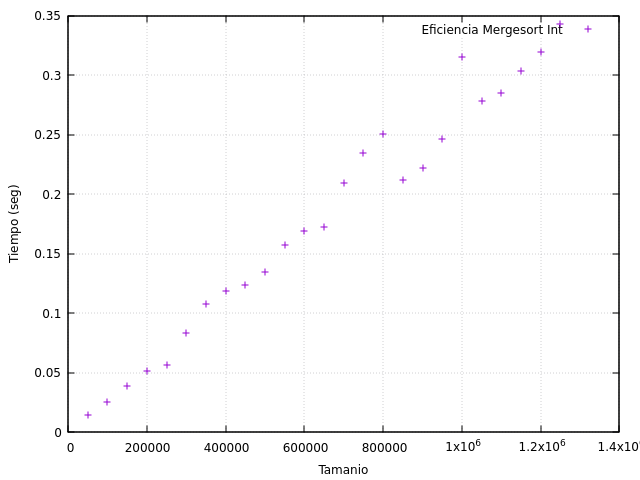
\includegraphics[width=0.8\linewidth]{images/Mergesort/Mergesort_Int_Graf.png}
        \cprotect\caption{Tiempo de ejecución Mergesort \verb|int| en PC Arturo.}
        \label{fig:Mergesort_int_graf}
    \end{figure}
    \begin{figure}
        \centering
        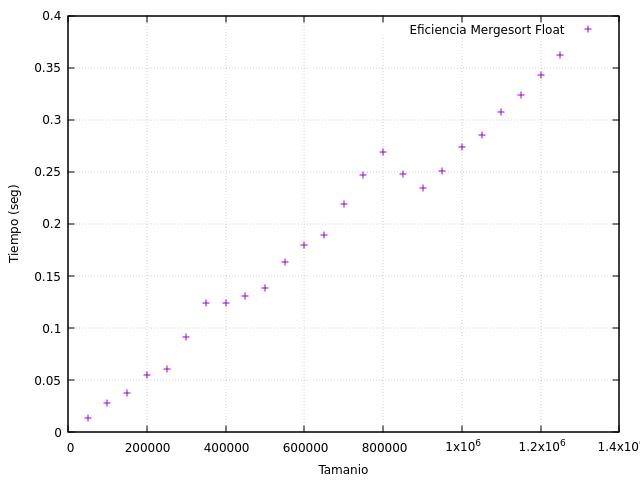
\includegraphics[width=0.8\linewidth]{images/Mergesort/Mergesort_Flt_Graf.png}
        \cprotect\caption{Tiempo de ejecución Mergesort \verb|float| en PC Arturo.}
        \label{fig:Mergesort_float_graf}
    \end{figure}
    \begin{figure}
        \centering
        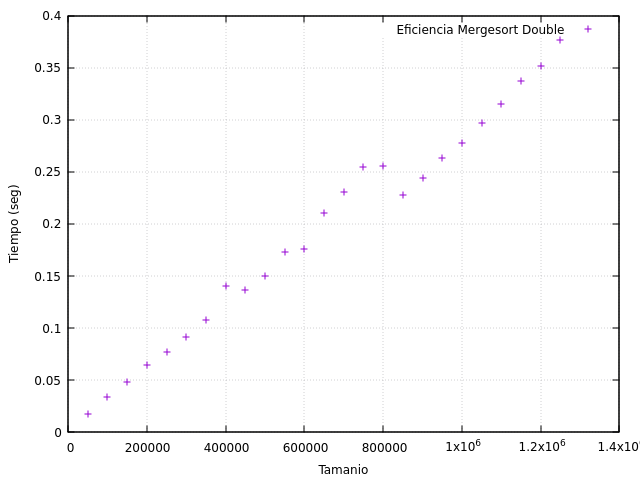
\includegraphics[width=0.8\linewidth]{images/Mergesort/Mergesort_Dbl_Graf.png}
        \cprotect\caption{Tiempo de ejecución Inserción \verb|double| en PC Arturo.}
        \label{fig:Mergesort_double_graf}
    \end{figure}
    \begin{figure}
        \centering
        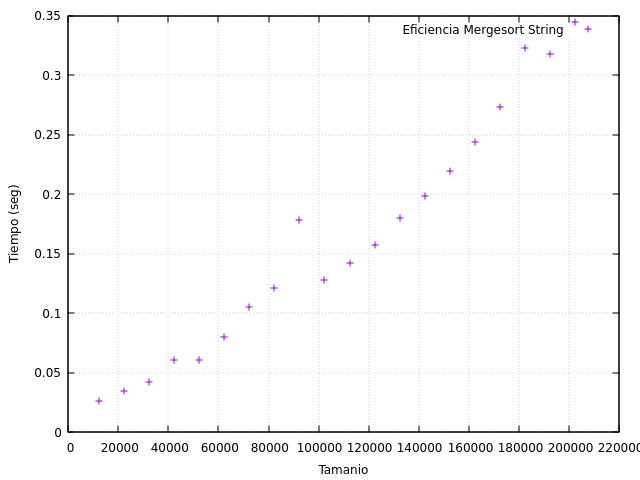
\includegraphics[width=0.8\linewidth]{images/Mergesort/Mergesort_Str_Graf.png}
        \cprotect\caption{Tiempo de ejecución Mergesort \verb|string| en PC Arturo.}
        \label{fig:Mergesort_string_graf}
    \end{figure}

    Sobre los mismos datos de la Tabla \ref{tab:Mergesort_tiempos} hemos realizado los siguientes ajustes, siendo todos linear-logarítmicos:

    \begin{itemize}
        \item Para \verb|ints|, se ha usado la función siguiente, que se observa en la Figura \ref{fig:MergesortRegresionInt}:
    $$f(x)=-0.0126508-7.72477\cdot 10^{-7}x-2.44202\cdot 10^{-8}x\log_2(x)$$

    \item Para \verb|float|, se ha usado la función siguiente, que se observa en la Figura \ref{fig:MergesortRegresionFloat}:
    $$f(x)=-0.0146428+9.2974\cdot 10^{-7}x-3.15744\cdot 10^{-8}x\log_2(x)$$

    \item Para \verb|double|, se ha usado la función siguiente, que se observa en la Figura \ref{fig:MergesortRegresionDouble}:
    $$f(x)=-0.00314742+7.17161\cdot 10^{-7}x-2.11266\cdot 10^{-8}x\log_2(x)$$

    \item Para \verb|string|, se ha usado la función siguiente, que se observa en la Figura \ref{fig:MergesortRegresionString}:
    $$f(x)=0.0389456-7.06717\cdot 10^{-6}x+4.84648\cdot 10^{-7}x\log_2(x)$$
    \end{itemize}

    \begin{figure}
        \centering
        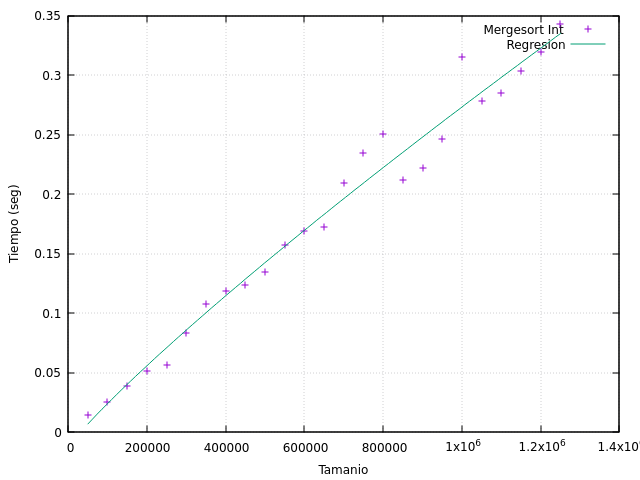
\includegraphics[width=0.8\linewidth]{images/Mergesort/Mergesort_Regresion_Int.png}
        \cprotect\caption{Regresión de Mergesort \verb|int| en PC Arturo.}
        \label{fig:MergesortRegresionInt}
    \end{figure}

    \begin{figure}
        \centering
        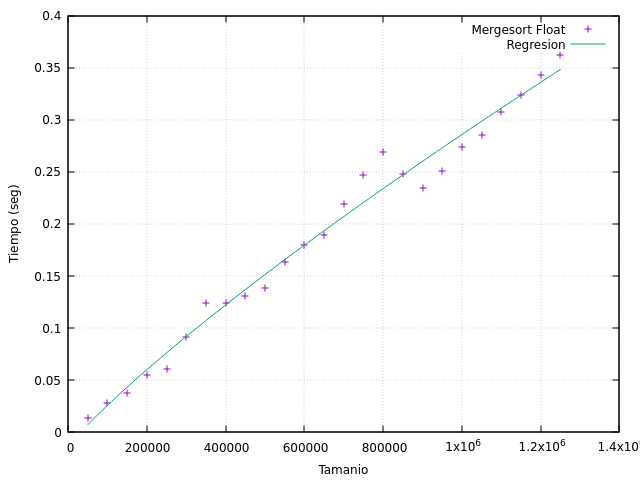
\includegraphics[width=0.8\linewidth]{images/Mergesort/Mergesort_Regresion_Flt.png}
        \cprotect\caption{Regresión de Mergesort \verb|float| en PC Arturo.}
        \label{fig:MergesortRegresionFloat}
    \end{figure}

    \begin{figure}
        \centering
        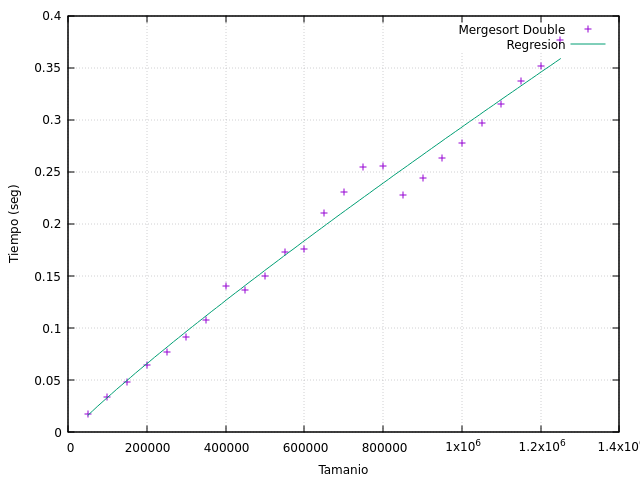
\includegraphics[width=0.8\linewidth]{images/Mergesort/Mergesort_Regresion_Dbl.png}
        \cprotect\caption{Regresión de Mergesort \verb|double| en PC Arturo.}
        \label{fig:MergesortRegresionDouble}
    \end{figure}

    \begin{figure}
        \centering
        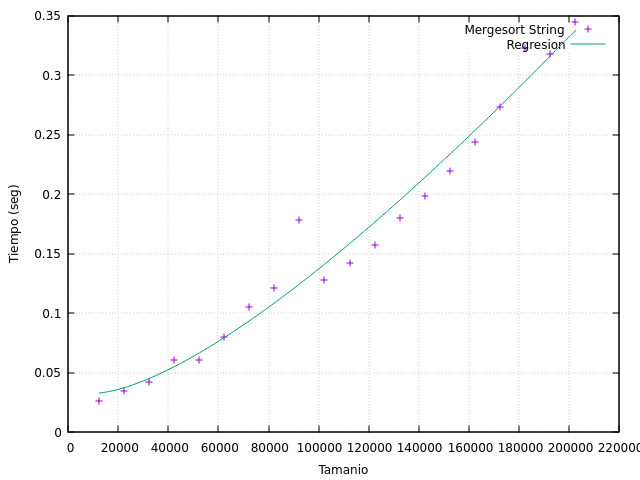
\includegraphics[width=0.8\linewidth]{images/Mergesort/Mergesort_Regresion_String.png}
        \cprotect\caption{Regresión de Mergesort \verb|string| en PC Arturo.}
        \label{fig:MergesortRegresionString}
    \end{figure}


    Por último, para concluir el estudio de la eficiencia empírica sobre este algoritmo de ordenación, en la Figura \ref{fig:ComparativaMergesortDatos} se han representado todos los tipos de datos para realizar una comparación de las mismas. Como se puede apreciar de forma directa, la ordenación en el caso de los \verb|string| es mucho más costosa, como ya hemos explicado en el presente documento. Un aspecto a destacar de esta gráfica son los picos de tiempo que se ven claramente en la Figura \ref{fig:ComparativaMergesortDatos}, especialmente para $n=400000$ y $n=800000$. Esto se debe a que el presente algoritmo requiere de grandes reservas de memoria en el Heap, y precisamente en dichos puntos seguramente requiera más espacio (o cualquier otro motivo de la gestión dinámica de la memoria) que implica estos picos.    
    \begin{figure}
        \centering
        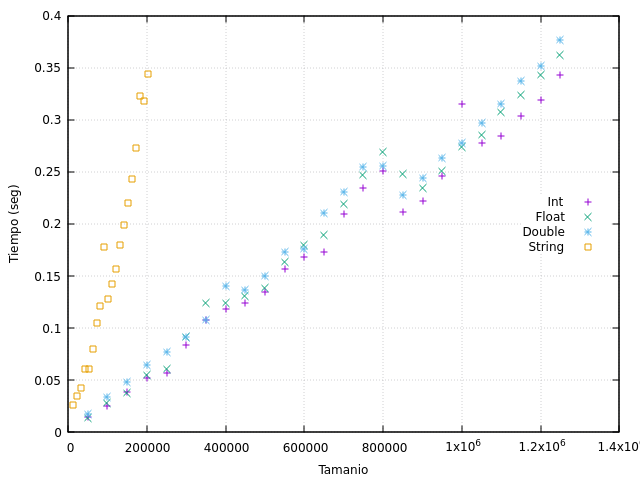
\includegraphics[width=0.8\linewidth]{images/Mergesort/Mergesort_Comparacion.png}
        \caption{Comparativos de tipos de datos del algoritmo Mergesort en el PC Arturo.}
        \label{fig:ComparativaMergesortDatos}
    \end{figure}\\
    
    \textbf{Quicksort}
    
    Tras ejecutar el algoritmo de Quicksort sobre datos aleatorios para tamaños de $n$ desde $50000$ hasta $1250000$ con saltos de $50000$ para los tipos de datos \verb|int|, \verb|double|, \verb|float|; y tamaños desde $12308$ hasta $202308$ con saltos de $10000$ para \verb|string|; obtenemos la Tabla \ref{tab:Quicksort_tiempos} de tiempos, donde en la columna $n$ indicamos el tamaño del problema y en las columnas de \verb|int|, \verb|double|, \verb|float| y \verb|string| indicamos el tiempo en segundos que tarda el algoritmo en ejecutarse según el tamaño de $n$ y del tipo de dato. Dichos resultados los podemos ver en las Figuras \ref{fig:Quicksort_int_graf}, \ref{fig:Quicksort_float_graf}, \ref{fig:Quicksort_double_graf} y \ref{fig:Quicksort_string_graf}.

    \begin{table}
        \centering
        \begin{tabular}{|l|l|l|l||l||l|l|}
             \hline
            $n$ & \verb|int| & \verb|double| & \verb|float| &\qquad\qquad& $n$ & \verb|string| \\
             \hline
             $50000$   & $0.00467381$ & $0.0114837$ & $0.0103696$ && $12308$  & $0.0220313$ \\
            $100000$  & $0.0098776 $ & $0.0121806$ & $0.0117013$ && $22308$  & $0.0229442$ \\
            $150000$  & $0.0156925 $ & $0.0183871$ & $0.018259$ && $32308$  & $0.0422547$ \\
            $200000$  & $0.0208121 $ & $0.0249882$ & $0.0247901$ && $42308$  & $0.06872$ \\
            $250000$  & $0.0265519 $ & $0.0319184$ & $0.0315846$ && $52308$  & $0.1012$ \\
            $300000$  & $0.0323268 $ & $0.038625 $ & $0.0383557$ && $62308$  & $0.142347$ \\
            $350000$  & $0.0379446 $ & $0.0455637$ & $0.0450607$ && $72308$  & $0.186687$ \\
            $400000$  & $0.0444629 $ & $0.0522814$ & $0.0517725$ && $82308$  & $0.241633$ \\
            $450000$  & $0.0496729 $ & $0.0598129$ & $0.059378$ && $92308$  & $0.295446$ \\
            $500000$  & $0.0561251 $ & $0.0668194$ & $0.0661963$ && $102308$ & $0.368751$ \\
            $550000$  & $0.0620964$  & $0.0742795$ & $0.0737543$ && $112308$ & $0.431337$ \\
            $600000$  & $0.0674103$  & $0.0812635$ & $0.0803504$ && $122308$ & $0.552277$ \\
            $650000$  & $0.0767052$  & $0.0892056$ & $0.0884973$ && $132308$ & $0.622159$ \\
            $700000$  & $0.0804308$  & $0.0950736$ & $0.0942522$ && $142308$ & $0.691106$ \\
            $750000$  & $0.0858259$  & $0.103554 $ & $0.102893$ && $152308$ & $0.806095$ \\
            $800000$  & $0.0913994$  & $0.110159 $ & $0.10909$ && $162308$ & $0.896376$ \\
            $850000$  & $0.095706 $  & $0.118214 $ & $0.116856$ && $172308$ & $1.01104$ \\
            $900000$  & $0.101631 $  & $0.125201 $ & $0.123795$ && $182308$ & $1.15227$ \\
            $950000$  & $0.108028 $  & $0.132181 $ & $0.130613$ && $192308$ & $1.27353$ \\
            $1000000$ & $0.111617$   & $0.140264$  & $0.138568$ && $202308$ & $1.4092 $\\
            $1100000$ & $0.1245    $ & $0.153546 $ & $0.152169$ && & \\
            $1150000$ & $0.131298  $ & $0.160642 $ & $0.158896$ && & \\
            $1200000$ & $0.13887   $ & $0.168724 $ & $0.166526$ && & \\
            $1250000$ & $0.146035  $ & $0.175753 $ & $0.174023$ && & \\
             \hline
        \end{tabular}
        \caption{Tiempos de ejecución para Quicksort en el ordenador de José Juan.}
        \label{tab:Quicksort_tiempos}
    \end{table}

    \begin{figure}
        \centering
        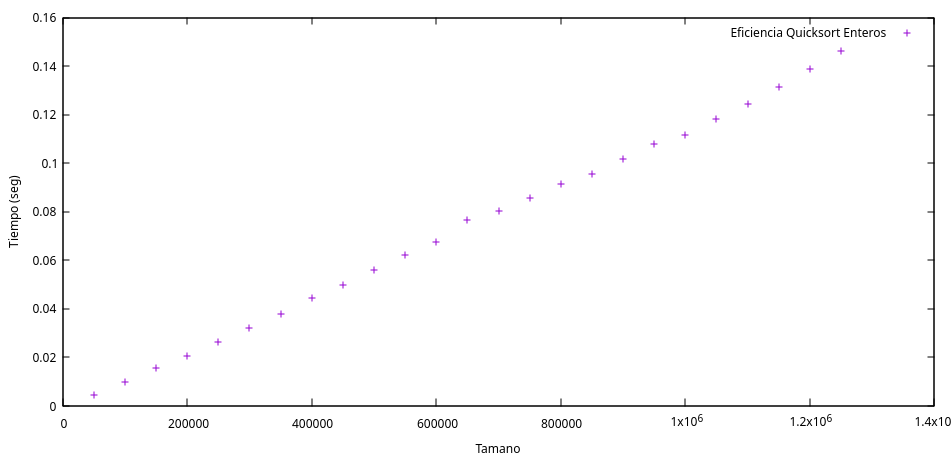
\includegraphics[width=\linewidth]{images/quicksort/graficas/quicksort-int-puntos.png}
        \cprotect\caption{Tiempo de ejecución de Quicksort para \verb|int| en PC José Juan.}
        \label{fig:Quicksort_int_graf}
    \end{figure}
    \begin{figure}
        \centering
        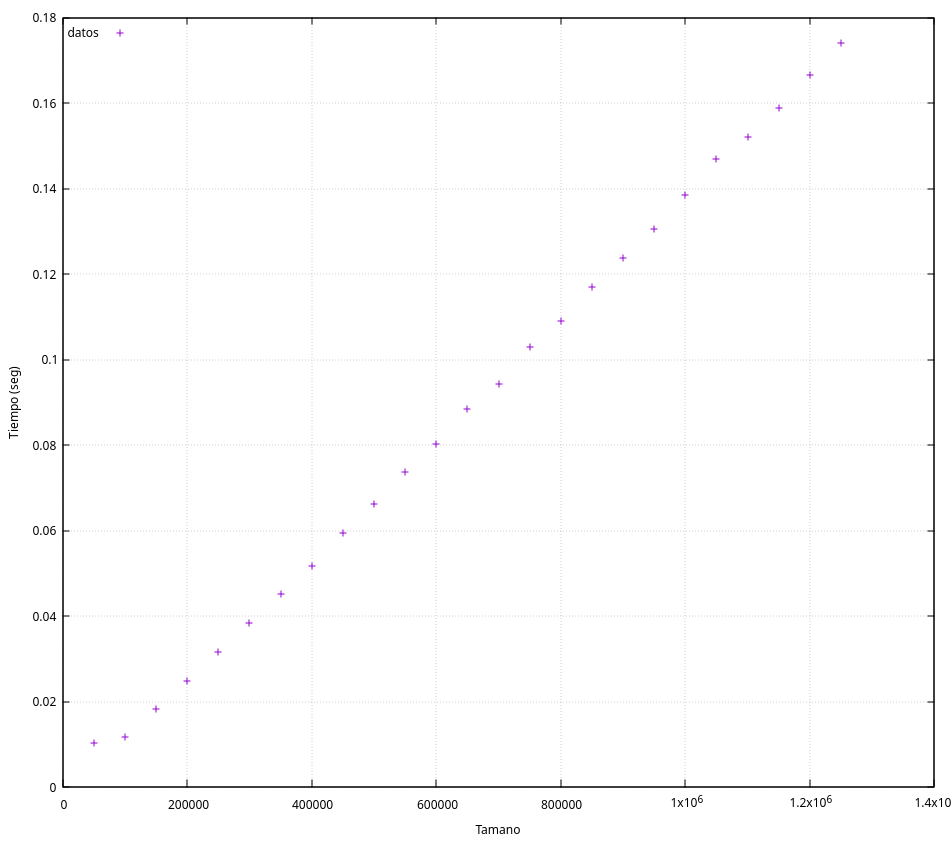
\includegraphics[width=0.8\linewidth]{images/quicksort/graficas/quicksort-float-puntos.png}
        \cprotect\caption{Tiempo de ejecución de Quicksort para \verb|float| en PC José Juan.}
        \label{fig:Quicksort_float_graf}
    \end{figure}
    \begin{figure}
        \centering
        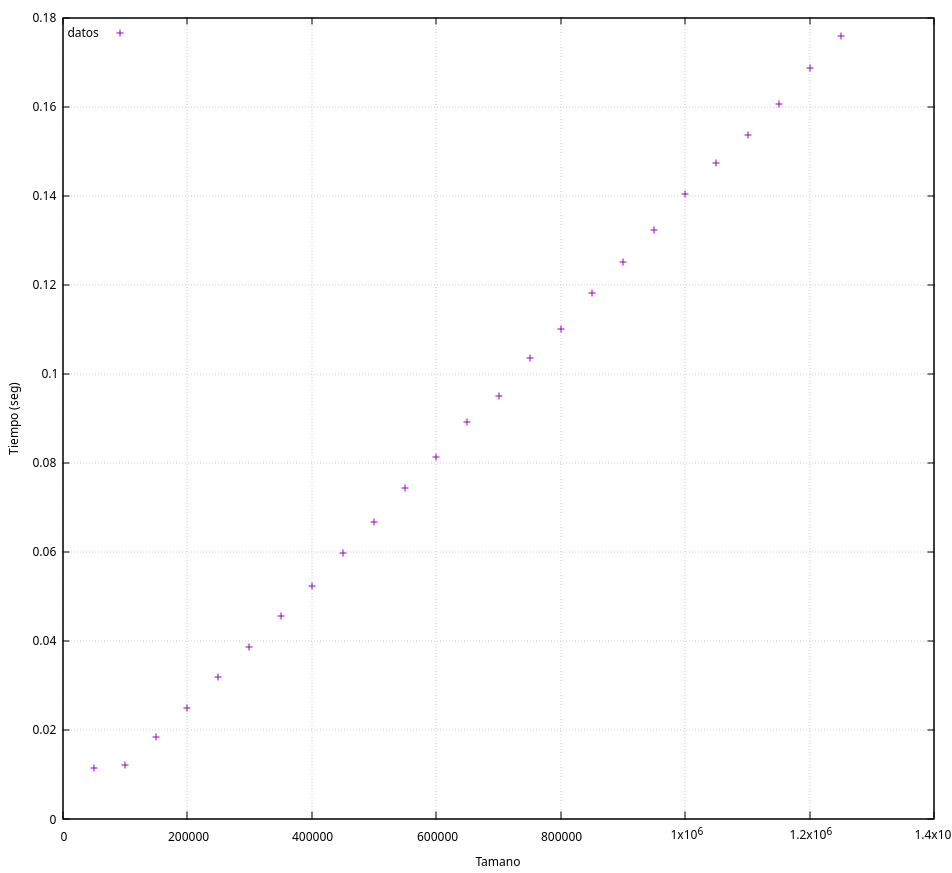
\includegraphics[width=0.8\linewidth]{images/quicksort/graficas/quicksort-double-puntos.png}
        \cprotect\caption{Tiempo de ejecución de Quicksort para \verb|double| en PC José Juan.}
        \label{fig:Quicksort_double_graf}
    \end{figure}
    \begin{figure}
        \centering
        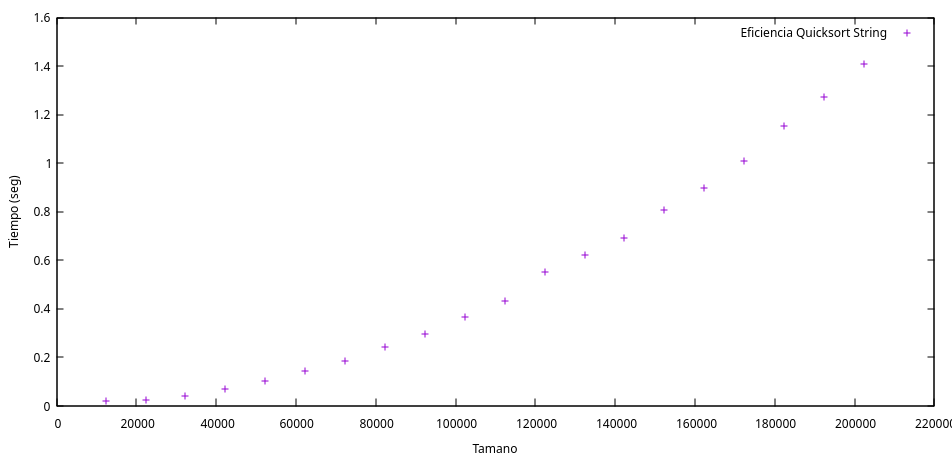
\includegraphics[width=\linewidth]{images/quicksort/graficas/quicksort-string-puntos.png}
        \cprotect\caption{Tiempo de ejecución de Quicksort para \verb|string| en PC José Juan.}
        \label{fig:Quicksort_string_graf}
    \end{figure}

    De estos datos vemos que a pesar de tener una complejidad del orden $O(n^2)$, el Quicksort presenta un crecimiento muy suave en el tiempo de ejecución respecto el tamaño de la entrada. Esto es debido a que es altamente improbable que se dé el peor caso del Quicksort salvo que intencionadamente se introduzcan datos que lo lleven a su peor tiempo de ejecución o que se use en situaciones inapropiadas, en las que un algoritmo como el de Inserción podría ser incluso mejor dependiendo del contexto (i.e. insertar al final nuevos datos en un vector ordenado y reordenar).
    
    Sabiendo que el Quicksort en su mejor caso es $O(n \log n)$ y observando las gráficas, vemos que no es disparatado pensar que casi siempre está más cerca de su mejor caso que de su peor caso. Para hacernos una idea de por qué esto es cierto vamos a razonar de manera intuitiva por qué este es el caso más probable: En el mejor caso del Quicksort, se partirá siempre a la mitad el vector y hará que se ejecute el algoritmo lineal de partir $\log(n)$ veces (aunque un poco antes cambiará el método de ordenación cuando los tamaños sean razonablemente pequeños debido a motivos de eficiencia). En su peor caso se partirá siempre el vector en un elemento aislado y otro vector con un elemento menos que el anterior; es en este caso en el que el Quicksort presenta una peor eficiencia. Esto ocurre cuando los datos ya están casi ordenados, ordenados en el orden contrario o se repiten demasiados datos. En ellos, se llama a \verb|dividir_qs| $n$ veces, una por cada dato.
    
    Podemos razonar entonces que, si no se aplica ninguna estrategia para evitar estos casos (que probablemente ni valdría la pena si el tiempo que tomara evaluar la estrategia no fuese muy pequeño), tendríamos que de vez en cuando se partiría el vector en dos subvectores de casi $\nicefrac{n}{2}$ y a veces solo se separarían unos pocos datos al partir. Entonces es razonable asumir que el vector es partido en $\nicefrac{n}{4}$ y en $\nicefrac{3n}{4}$ si queremos hacer un análisis de cómo se comportaría en un caso promedio. Esta es una asunción algo simple, pero nos ayudará a entender cuan rápido es en media el Quicksort. 
    Como los vectores se dividen en $\nicefrac{1}{4}$ y en $\nicefrac{3}{4}$ de su tamaño original, la intuición nos dice que en la parte de un cuarto del tamaño original se llega al final en $\log_4(n)$. En la parte de tres cuartos se llega al final en $\log_{\nicefrac{4}{3}}(n)$. En esta premisa, tenemos que ambos logaritmos son equivalentes por una constante real, así que nos encontramos en un caso muy parecido en orden de eficiencia al mejor caso. Esta es la intuición que hay detrás de que el Quicksort sea en media de orden $O(n \log n)$. (La demostración rigurosa de esto es complicada y se sale del propósito de la asignatura, que se centra más en el peor caso).
    

    Sobre los mismos datos de la Tabla \ref{tab:Quicksort_tiempos} hemos realizado los siguientes ajustes (que corresponden con el mejor ajuste en cada caso), siendo todos linear-logarítimicos (es el ajuste adecuado según el razonamiento anterior) salvo para \verb|string|:
    \begin{itemize}
        \item Para \verb|int|, se ha usado la función siguiente, que se observa en la Figura \ref{fig:RegresionQuicksortInt}:
        $$f(x)=-0.00130275+9.59332\cdot 10^{-8}x + 1.02604\cdot 10^{-9}x\log_2(x)$$
    
        \item Para \verb|float|, se ha usado la función siguiente, que se observa en la Figura \ref{fig:RegresionQuicksortFloat}:
        $$f(x)=0.00178712-5.31219\cdot 10^{-9} x+7.09756\cdot 10^{-9}x\log_2(x)$$
    
        \item Para \verb|double|, se ha usado la función siguiente, que se observa en la Figura \ref{fig:RegresionQuicksortDouble}:
        $$f(x)=0.00264789-2.75117\cdot 10^{-8}x +8.2366\cdot 10^{-9}x\log_2(x)$$
    
        \item Para \verb|string|, se ha usado la función siguiente, que se observa en la Figura \ref{fig:RegresionQuicksortString}:
        $$f(x)=0.00809874+4.84326\cdot 10^{-8} x+3.39336\cdot 10^{-11} x^2$$
    \end{itemize}

    \begin{figure}
        \centering
        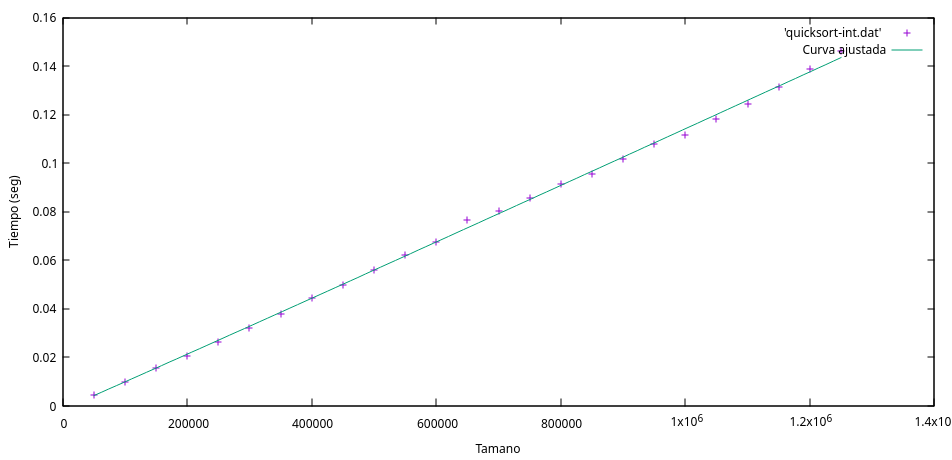
\includegraphics[width=\linewidth]{images/quicksort/graficas/quicksort-int-regresion.png}
        \cprotect\caption{Regresión del algoritmo Quicksort para \verb|int| en el PC de José Juan.}
        \label{fig:RegresionQuicksortInt}
    \end{figure}
    \begin{figure}
        \centering
        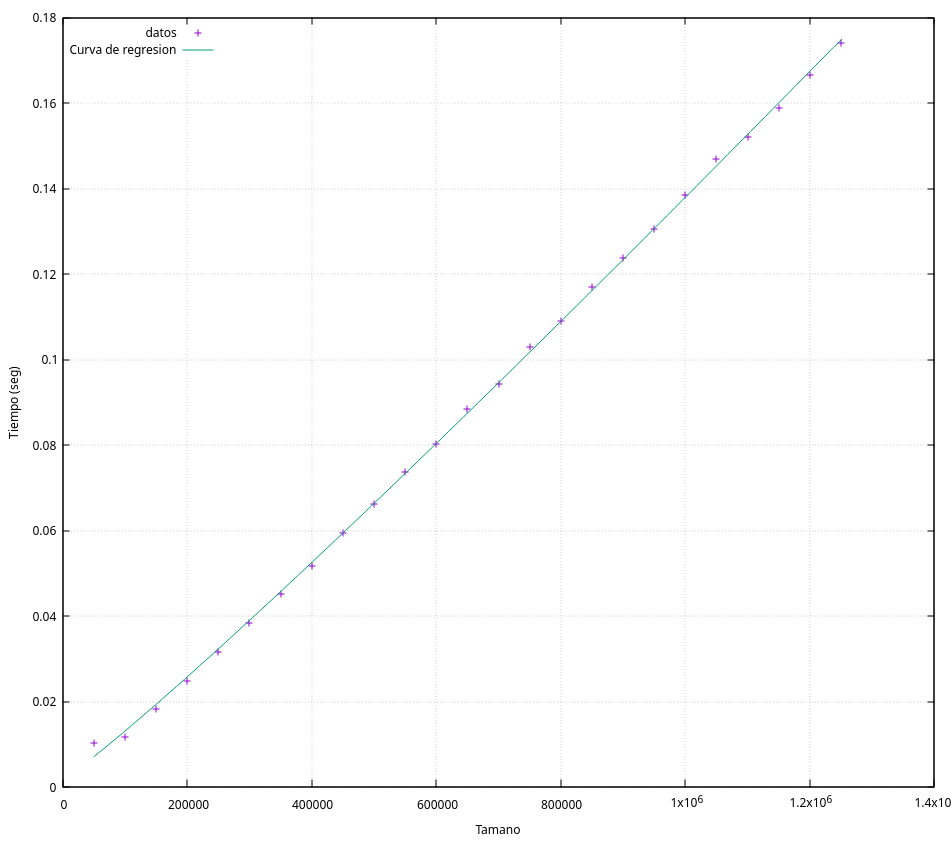
\includegraphics[width=0.8\linewidth]{images/quicksort/graficas/quicksort-float-regresion.png}
        \cprotect\caption{Regresión del algoritmo Quicksort para \verb|float| en el PC de José Juan.}
        \label{fig:RegresionQuicksortFloat}
    \end{figure}
    \begin{figure}
        \centering
        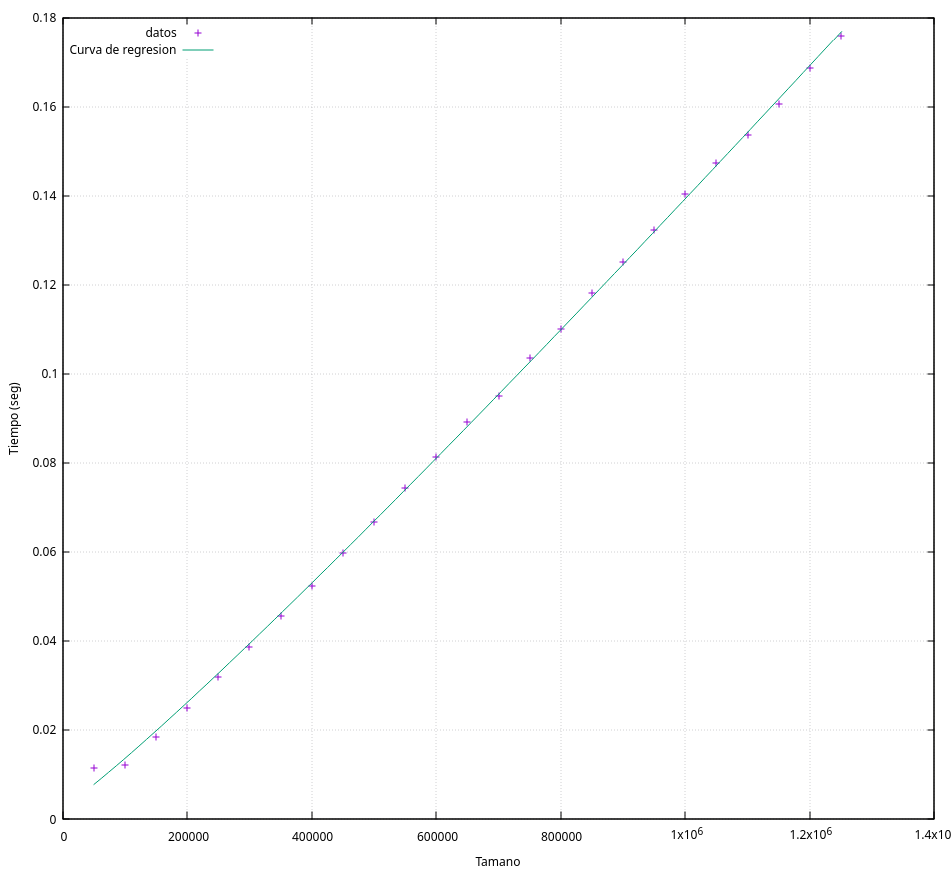
\includegraphics[width=0.8\linewidth]{images/quicksort/graficas/quicksort-double-regresion.png}
        \cprotect\caption{Regresión del algoritmo Quicksort para \verb|double| en el PC de José Juan.}
        \label{fig:RegresionQuicksortDouble}
    \end{figure}
    \begin{figure}
        \centering
        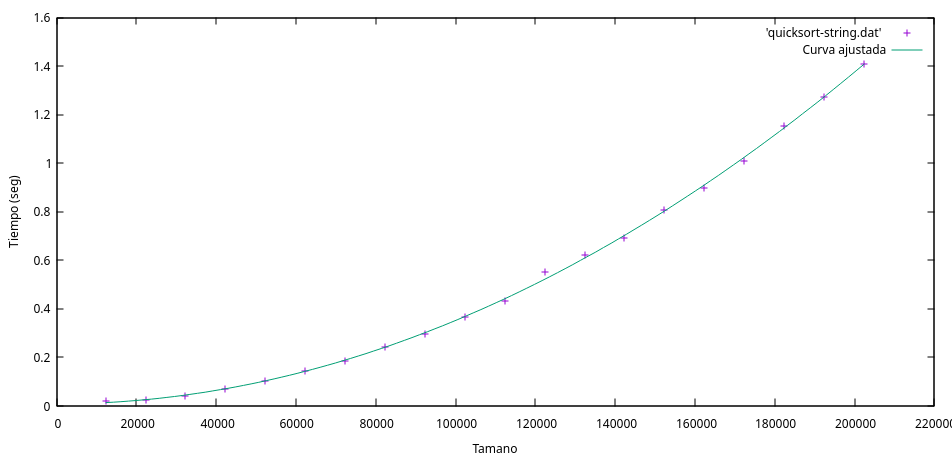
\includegraphics[width=\linewidth]{images/quicksort/graficas/quicksort-string-regresion.png}
        \cprotect\caption{Regresión del algoritmo Quicksort para \verb|string| en el PC de José Juan.}
        \label{fig:RegresionQuicksortString}
    \end{figure}
    \begin{figure}
        \centering
        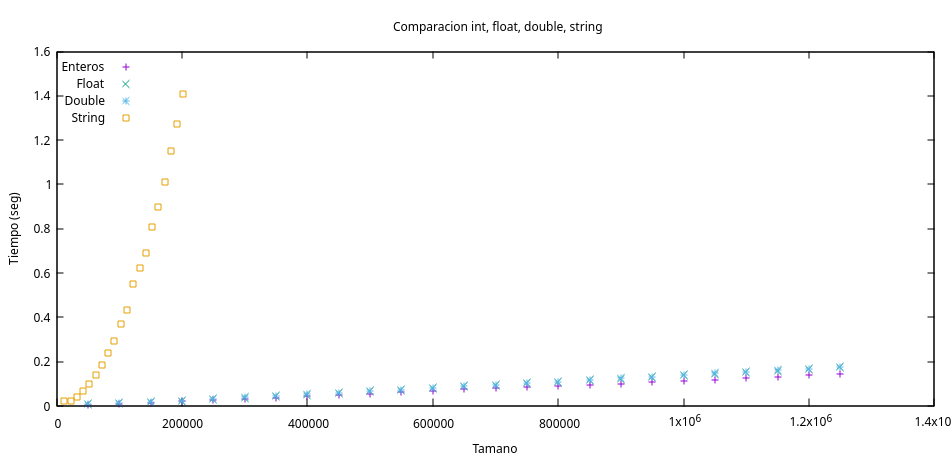
\includegraphics[width=\linewidth]{images/quicksort/graficas/Comparativa.png}
        \caption{Comparativa de tipos de datos del algoritmo Quicksort en PC José Juan.}
        \label{fig:QuicksortComparativaDatos}
    \end{figure}

    En la Figura \ref{fig:QuicksortComparativaDatos}, comparamos la influencia del cambio de tipos de datos. Como cabría esperar, \verb|int| es el tipo que proporciona la ejecución más liviana. Los tipos de datos \verb|float| y \verb|double| están bastante cerca en cuanto a tiempo de ejecución y, con \verb|string|, observamos algo novedoso: el comportamiento del algoritmo cambia de $n\log(n)$ a $n^2$. Para corroborarlo, podemos observar la Figura \ref{fig:QuicksortComparativaString}. En ella claramente se observa que el ajuste cuadrático es mejor que el linear-logarítmico. Realizando el análisis teórico de Quicksort, observábamos que este tiene un orden de eficiencia de $O(n^2)$ en su peor caso (que estén los datos casi ordenados) y $O(n\log n)$ en el caso promedio. Hemos podido ver que para valores aleatorios de \verb|int|, \verb|float| y \verb|double| el algoritmo presenta un orden de eficiencia $O(n\log n)$, como cabría esperar al ser datos aleatorios y, por tanto, podemos imaginar que se ajustarían a una instancia de caso promedio. Sin embargo, con \verb|string| observamos un comportamiento novedoso: el orden de eficiencia del algoritmo pasa a ser de $O(n^2)$, algo que no esperábamos, ya que los datos de entrada son de un libro, contienen multitud de palabras y podríamos pensar que se asemejaría a generar palabras de forma aleatoria. Sabemos que las operaciones de comparación e intercambio de \verb|string| son más costosas, pero no deberían cambiar el orden de eficiencia del algoritmo (ya que dichas operaciones son del orden $O(m)$ siendo $m$ el tamaño de la palabra, que de media en español es de $5$ letras, en comparación con el tamaño de $n$, que varía desde $12308$ hasta $202308$, luego $m<<n$). ¿A qué se debe este cambio en el orden de eficiencia de Quicksort?

    Pues se debe a que no estamos considerando cadenas aleatorias (como cabría esperar), estamos considerando palabras aleatorias \emph{en español}. Según Wikipedia, la distribución de las letras en español se corresponde con la Tabla \ref{tab:freq_wikipedia}, que podemos ver gráficamente en la Figura \ref{fig:freq_wikipedia} (excluimos la ``ñ'' debido a que su código ASCII no está entre el de la ``a'' y la ``z''), donde podemos ver que de las $26$ letras consideradas, $10$ no aparecen ni el $1\%$ de las veces, mientras que la ``a'' y la ``e'' aparecen más del $12\%$ cada una. Esta diferencia hace que el Quicksort trate de ordenar una instancia que no corresponde con el caso promedio, sino con el peor caso. Para corroborarlo, en la Tabla \ref{tab:freq_wikipedia} representamos además la cantidad de palabras del Quijote (libro que tomamos como banco de palabras para \verb|string|) que empiezan con cada letra (por cómo se ordenan las palabras, es más relevante ver por qué letra comienzan que la frecuencia de las letras en las palabras). Podemos visualizar esta cantidad gracias a la Figura \ref{fig:cant_quijote}.
    
    \begin{figure}
        \centering
        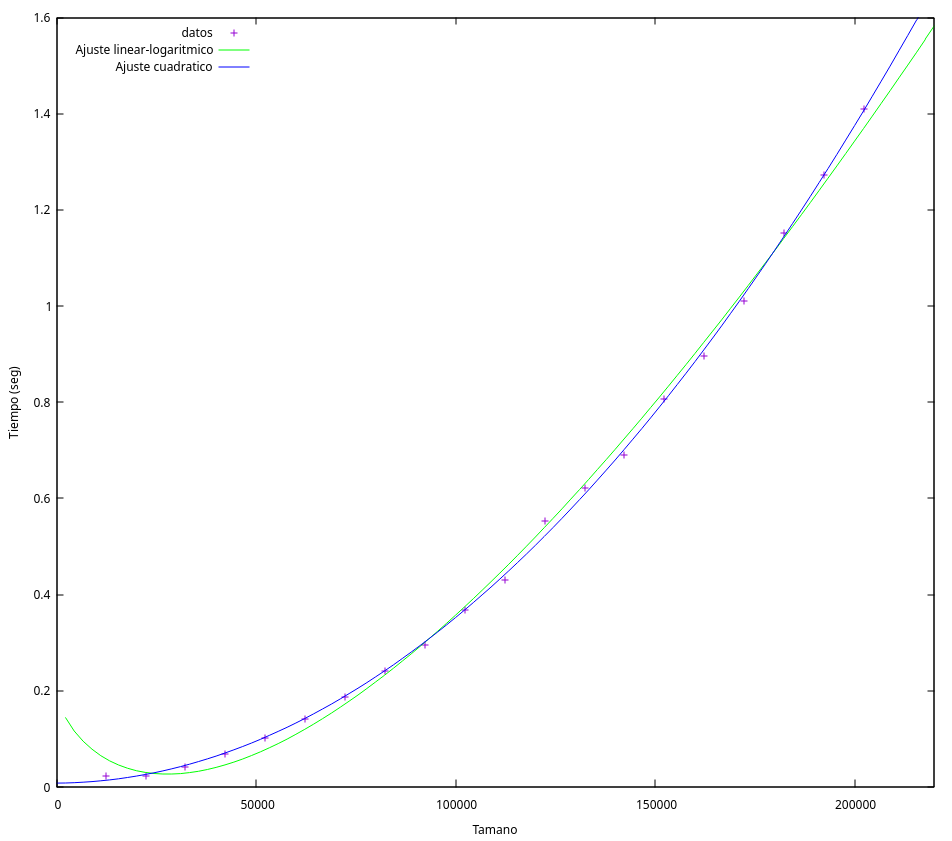
\includegraphics[width=\linewidth]{images/quicksort/graficas/string/Comparativa-ajustes.png}
        \cprotect\caption{Comparativa de tipos de ajuste para \verb|string| en PC José Juan.}
        \label{fig:QuicksortComparativaString}
    \end{figure}
    \begin{table}
        \centering
        \begin{tabular}{|c|l|l|}
            \hline
            Letra & Frecuencia & Palabras que empiezan\\
            & (en porcentaje) & por cada letra en el Quijote\\
            \hline
            a & $12.53$ & $16141$ \\
            b & $1.42$ & $2803$ \\
            c & $4.68$ & $14441$ \\
            d & $5.86$ & $22108$ \\
            e & $13.68$ & $18046$ \\
            f & $0.69$ & $2954$ \\
            g & $1.01$ & $1851$ \\
            h & $0.7$ & $6723$ \\
            i & $6.25$ & $1462$ \\
            j & $0.44$ & $676$ \\
            k & $0.02$ & $0$ \\
            l & $4.97$ & $17220$ \\
            m & $3.15$ & $11038$ \\
            n & $6.71$ & $6001$ \\
            o & $8.68$ & $3134$ \\
            p & $2.51$ & $13314$ \\
            q & $0.88$ & $14657$ \\
            r & $6.87$ & $2967$ \\
            s & $7.98$ & $15369$ \\
            t & $4.63$ & $8019$ \\
            u & $3.93$ & $2024$ \\
            v & $0.9$ & $5744$ \\
            w & $0.01$ & $8$ \\
            x & $0.22$ & $42$ \\
            y & $0.9$ & $10791$ \\
            z & $0.52$ & $141$ \\
            \hline
        \end{tabular}
        \caption{\centering Tabla de análisis de frecuencia de aparición de letras según Wikipedia y de comienzo de palabras en español según el Quijote.}
        \label{tab:freq_wikipedia}
    \end{table}
    \begin{figure}
        \centering
        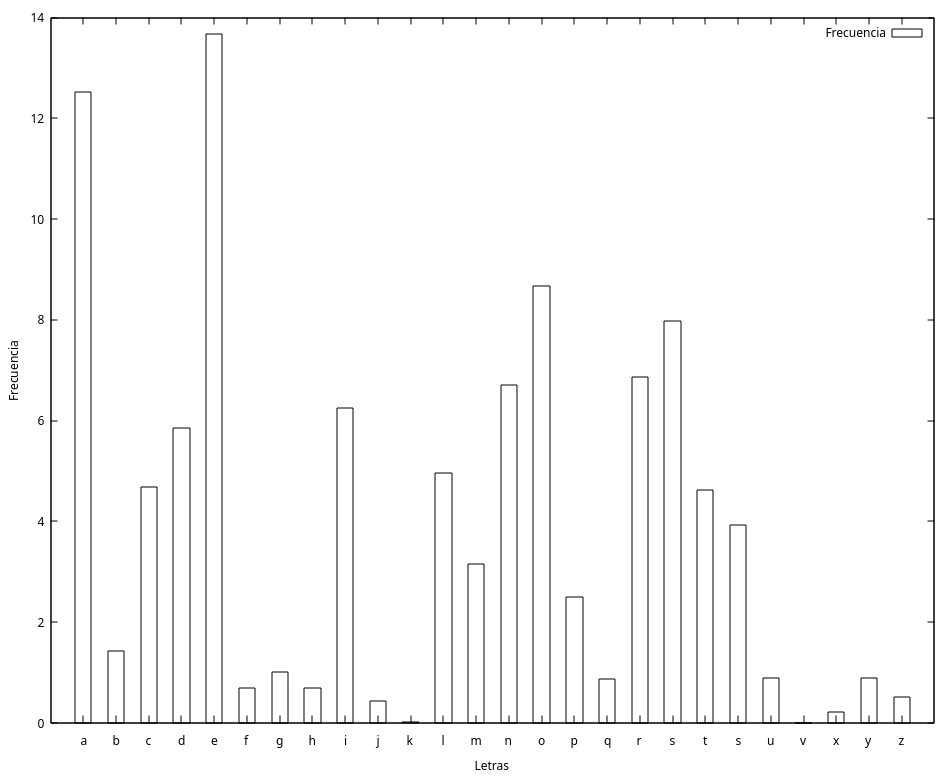
\includegraphics[width=0.8\linewidth]{images/quicksort/graficas/string/Frecuencia-letras.png}
        \cprotect\caption{Frecuencia de aparición de letras en español según Wikipedia.}
        \label{fig:freq_wikipedia}
    \end{figure}
    \begin{figure}
        \centering
        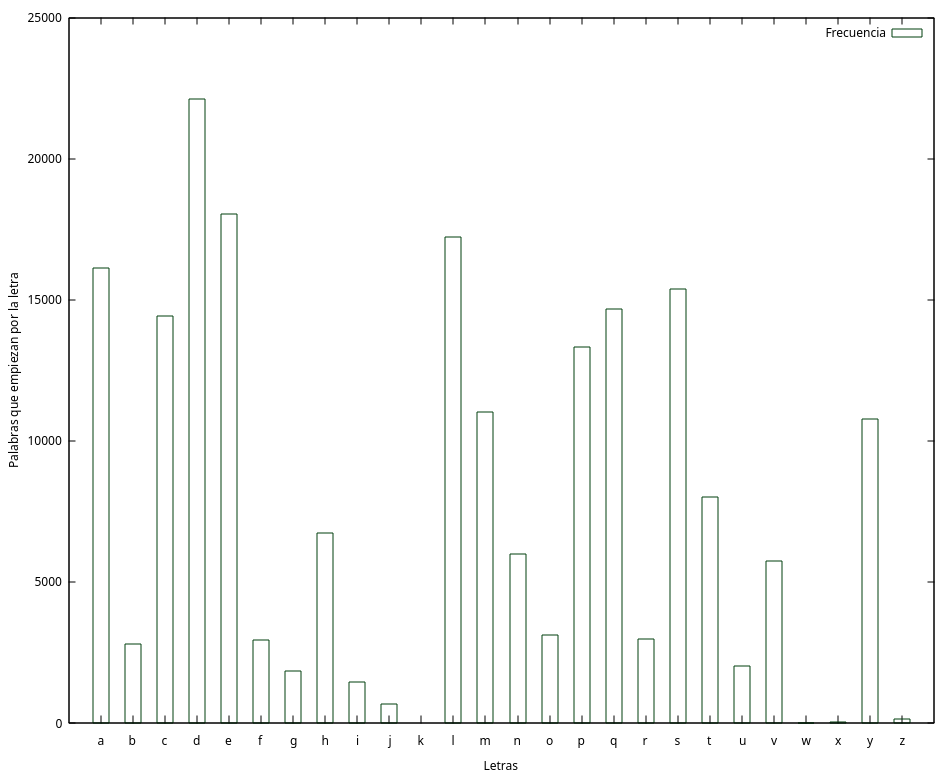
\includegraphics[width=0.8\linewidth]{images/quicksort/graficas/string/Frecuencia-quijote.png}
        \cprotect\caption{Cantidad de palabras que comienzan por cada letra en el Quijote.}
        \label{fig:cant_quijote}
    \end{figure}
    
    
    \subsubsection{Comparación de algoritmos linear-logarítmicos}

    \begin{table}
        \centering
        \begin{tabular}{|c|c|c|}
            \hline
            $n$ & Mergesort & Quicksort \\
            \hline
            $50000$   & $0.006236$ & $0.00345248$ \\
            $100000$  & $0.013314$ & $0.00701012$ \\
            $150000$  & $0.019333$ & $0.0115228$ \\
            $200000$  & $0.028895$ & $0.0154378$ \\
            $250000$  & $0.0317$ & $0.0194958$ \\
            $300000$  & $0.041888$ & $0.0232022$ \\
            $350000$  & $0.050927$ & $0.0284878$ \\
            $400000$  & $0.060585$ & $0.0318925$ \\
            $450000$  & $0.059927$ & $0.0364872$ \\
            $500000$  & $0.069133$ & $0.0416348$ \\
            $550000$  & $0.076643$ & $0.0450575$ \\
            $600000$  & $0.085745$ & $0.049795$ \\
            $650000$  & $0.096291$ & $0.0545303$ \\
            $700000$  & $0.1036$ & $0.0603586$ \\
            $750000$  & $0.116193$ & $0.0631069$ \\
            $800000$  & $0.128549$ & $0.0680165$ \\
            $850000$  & $0.120082$ & $0.0725883$ \\
            $900000$  & $0.127915$ & $0.0771059$ \\
            $950000$  & $0.136794$ & $0.0813733$ \\
            $1000000$ & $0.141584$ & $0.0864082$ \\
            $1050000$ & $0.154477$ & $0.0913727$ \\
            $1100000$ & $0.162778$ & $0.0960989$ \\
            $1150000$ & $0.169551$ & $0.0988133$ \\
            $1200000$ & $0.178112$ & $0.102367$ \\
            $1250000$ & $0.187529$ & $0.107923$ \\
            \hline
        \end{tabular}
        \caption{Tabla comparativa del Mergesort y Quicksort en PC Irina.}
        \label{tab:merge_quick}
    \end{table}

    \begin{figure}
        \centering
        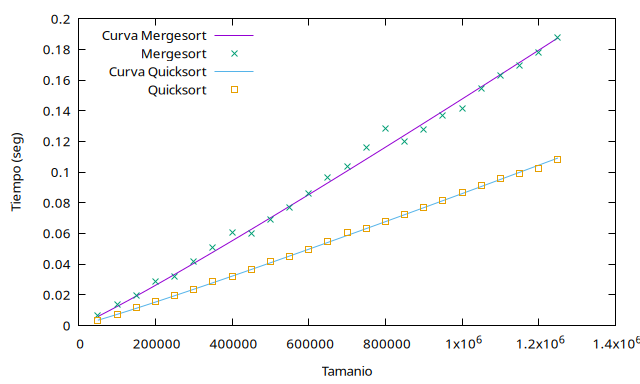
\includegraphics[width=\linewidth]{images/Comparaciones/merge_quick.png}
        \caption{Comparativa de los algoritmos linear-logarítmicos en el PC Irina.}
        \label{fig:merge_quick}
    \end{figure}

    Como se puede observar en los datos recogidos de la Tabla~\ref{tab:merge_quick}, el Mergesort se ejecuta casi $1.7$ veces peor que el Quicksort. Esto es, entre otras cosas, debido a que nuestra versión del Mergesort requiere una cantidad $n \log(n)$ de memoria auxiliar, la cual reserva de manera dinámica. Esto causa que el algoritmo sea bastante más lento que el Quicksort en su caso medio, que tan solo requiere un almacenamiento auxiliar constante. Sin embargo, es de vital importancia resaltar que el Quicksort ha ganado en tiempo debido a que recibió una entrada aleatoria con el propósito de visualizar el caso medio. En su peor caso, como ya hemos resaltado bastantes veces, el Quicksort  es $O(n^2)$, lo que causaría que, en un caso malo del Quicksort, el algoritmo perdiese estrepitosamente la comparación de cuál de los dos es más rápido. 
    En la Figura \ref{fig:merge_quick} se ilustra de manera más visual cómo evoluciona esta diferencia a lo largo del tiempo, lo que nos permite ver que el Quicksort aun así es la mejor elección en su caso medio. Sin embargo, se debe decidir de forma coherente cuál de los dos usar en cada caso, pues Quicksort debe quedar descartado si se van a ordenar datos casi ordenados o muchos datos repetidos, ya que estos son algunos de sus peores casos. 
    
    Mientras tanto, el Mergesort con esta implementación debe evitar ser usado si pueden haber limitaciones en la memoria principal disponible; como puede darse el caso en sistemas empotrados en los que, por algún motivo, se necesite ordenar muchos datos o en algunos sistemas en concreto de tiempo real, pues esto podría causar que se bloqueen procesos (Swapping) para poder ordenar rápidamente, o se tendría que realizar muchas peticiones de E/S para poder usar la memoria secundaria para ordenar. En un sistema de tiempo real esto podría traer consecuencias nefastas, así que en estos casos concretos el Quicksort sería una mejor elección. 
    
    \subsubsection{Comparación en distinto hardware}
    Como algoritmo linear-logarítmico para ejecutarse en todos los ordenadores hemos elegido el algoritmo de Quicksort. Mostramos ahora en la Tabla \ref{tab:comp_hardware_quicksort} los tiempos de ejecución en cada uno de los ordenadores y lo resaltamos gráficamente en la Figura \ref{fig:CompHardwareQuicksort}.
    \begin{table}
        \centering
        \begin{tabular}{|l|l|l|l|l|l|}
            \hline
            $n$ & José Juan & Arturo & Irina & Lucas & Airam \\
            \hline
            $50000$ & $0.0042545$ & $0.00996516$ & $0.00335371$ & $0.00532395$ & $0.0132008$ \\
            $100000$ & $0.0095564$ & $0.0179203$ & $0.00711646$ & $0.0110067$ & $0.0278678$ \\
            $150000$ & $0.0140981$ & $0.0242093$ & $0.0112455$ & $0.0163917$ & $0.0428819$ \\
            $200000$ & $0.0205965$ & $0.0308087$ & $0.0155371$ & $0.0198361$ & $0.056683$ \\
            $250000$ & $0.0262451$ & $0.0378297$ & $0.0194076$ & $0.0247633$ & $0.0685042$ \\
            $300000$ & $0.0318026$ & $0.0457154$ & $0.023623$ & $0.0297904$ & $0.0867636$ \\
            $350000$ & $0.0372646$ & $0.0545872$ & $0.0278431$ & $0.0353328$ & $0.0987438$ \\
            $400000$ & $0.0430272$ & $0.0630784$ & $0.0317653$ & $0.0404795$ & $0.113244$ \\
            $450000$ & $0.0485389$ & $0.0707236$ & $0.0369531$ & $0.0459344$ & $0.126802$ \\
            $500000$ & $0.0542375$ & $0.0799438$ & $0.0416354$ & $0.0513512$ & $0.150223$ \\
            $550000$ & $0.0601134$ & $0.0922267$ & $0.0448741$ & $0.0578232$ & $0.159226$ \\
            $600000$ & $0.066169$ & $0.0969197$ & $0.049937$ & $0.0641938$ & $0.17775$ \\
            $650000$ & $0.0708353$ & $0.103708$ & $0.0533011$ & $0.0688807$ & $0.185832$ \\
            $700000$ & $0.0772646$ & $0.113966$ & $0.0594714$ & $0.0751388$ & $0.201091$ \\
            $750000$ & $0.0839523$ & $0.128006$ & $0.0628564$ & $0.0815278$ & $0.22947$ \\
            $800000$ & $0.0898418$ & $0.12998$ & $0.0686097$ & $0.0853565$ & $0.234128$ \\
            $850000$ & $0.0959496$ & $0.139148$ & $0.0705088$ & $0.0921127$ & $0.247716$ \\
            $900000$ & $0.101498$ & $0.14925$ & $0.0749372$ & $0.0970982$ & $0.263426$ \\
            $950000$ & $0.1077$ & $0.158863$ & $0.0824308$ & $0.103748$ & $0.295789$ \\
            $1000000$ & $0.113698$ & $0.165685$ & $0.0864631$ & $0.110242$ & $0.303211$ \\
            $1050000$ & $0.120464$ & $0.177278$ & $0.0922949$ & $0.116239$ & $0.309282$ \\
            $1100000$ & $0.125074$ & $0.183784$ & $0.0985157$ & $0.123108$ & $0.329378$ \\
            $1150000$ & $0.131339$ & $0.194812$ & $0.101853$ & $0.12938$ & $0.344027$ \\
            $1200000$ & $0.137853$ & $0.201575$ & $0.105796$ & $0.133816$ & $0.378104$ \\
            $1250000$ & $0.144411$ & $0.212129$ & $0.108373$ & $0.143624$ & $0.381028$ \\
            \hline
        \end{tabular}
        \caption{Comparación Quicksort en distinto hardware.}
        \label{tab:comp_hardware_quicksort}
    \end{table}
    \begin{figure}
        \centering
        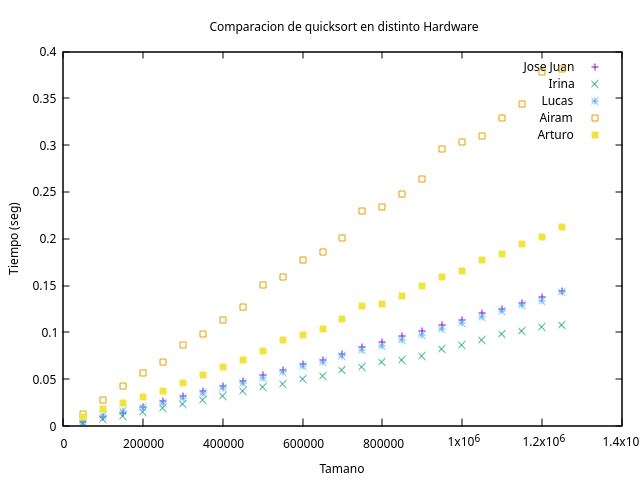
\includegraphics[width=0.8\linewidth]{images/Comparaciones_hardware/Comparacion_hardware_quicksort.png}
        \caption{Quicksort en todos los PCs.}
        \label{fig:CompHardwareQuicksort}
    \end{figure}

    En los datos de la Figura \ref{fig:CompHardwareQuicksort} observamos cómo la diferencia de tiempos de ejecución entre cualesquiera dos ejecuciones del mismo tamaño de entrada está determinado por una constante. Por ejemplo, la diferencia de tiempo de ejecución entre el ordenador de José Juan y el ordenador de Airam nos muestra que el ordenador de José Juan corre aproximadamente $2.7$ veces más rápido el Quicksort que el ordenador de Airam. Cabe destacar que a pesar de tener las mismas prestaciones, el ordenador de Lucas y el ordenador de Airam presentan tiempos muy dispares. Como el algoritmo se ejecuta de forma secuencial, hemos descartado la posibilidad de que sea por una diferencia en el número de cores disponibles. 

    En todos los ordenadores, no obstante, se aprecia como el tiempo de ejecución crece de forma casi lineal con respecto a su entrada (sabemos, sin embargo, que una curva lineal-logarítmica explica mucho mejor los resultados, a pesar de que a simple vista sea difícil de apreciar). Esto nos muestra cómo el Quicksort es un algoritmo que no requiere de un hardware específico para comportarse de una manera bastante estable en el caso medio. Deducimos también que es un buen algoritmo que usar cuando se quieren ordenar datos de tamaño razonablemente grande incluso en nuestros ordenadores portátiles, lo que lo hace un algoritmo adecuado para utilizar en ámbitos que requieran ordenar 2 o 3 millones de datos en un corto periodo de tiempo. Nótese que, de ser estrictamente necesario reducir el tiempo de cómputo, se puede desarrollar un algoritmo multihebra para que al partir los datos se asigne cada subvector a un hilo y acelerar considerablemente el tiempo de ejecución.

    \subsection{Algoritmos cúbicos}
    Esta sección trata sobre el algoritmo de Floyd, que calcula el coste mínimo de caminos en un grafo. Se trata del único algoritmo cúbico que tratamos en este estudio.
    \subsubsection{Análisis teórico}
    \textbf{Floyd}
    
    El código del algoritmo se encuentra en el Código fuente \ref{code:Floyd}.
    \begin{listing}
        \begin{minted}[linenos,xleftmargin=2cm]{c++}
void Floyd(int **M, int dim){
    for(int k = 0; k < dim; k++)
        for(int i = 0; i < dim; i++)
            for(int j = 0; j < dim; j++){
                int sum = M[i][k] + M[k][j];
                M[i][j] = (M[i][j] > sum)? sum : M[i][j];
            }
}
        \end{minted}
        \caption{Algoritmo de Floyd.}
        \label{code:Floyd}
    \end{listing}
    
    
    El tiempo de ejecución de las líneas 5 y 6 pueden acotarse por una constante, que denotaremos por $a$, debido a que su tiempo de ejecución no depende del tamaño de $dim$, que es la dimensión de nuestro problema, la cual denotaremos por $n$ para abreviar. Teniendo esto en cuenta, procedemos a calcular el tiempo de ejecución en función de la constante $a$:
    $$T(n)=\sum_{k=0}^{n-1} \sum_{i=0}^{n-1} \sum_{j=0}^{n-1} a = a \sum_{k=1}^n \sum_{i=1}^n \sum_{j=1}^n 1 = a\sum_{k=1}^n \sum_{i=1}^n n =a \sum_{k=1}^n n^2 = a \cdot n^3$$
    El algoritmo por tanto tiene un tiempo de ejecución $T(n) = a\cdot n^3$, que claramente es de orden $O(n^3)$.
    \subsubsection{Análisis empírico e híbrido}
    \textbf{Floyd}

    Tras ejecutar el algoritmo de Floyd para tamaños de $n$ de $50$ a $1250$ con saltos de $50$, obtenemos la Tabla \ref{tab:Floyd_tiempos} que relaciona el tamaño de $n$ con su tiempo de ejecución en segundos. Representamos estos datos en la gráfica de la Figura \ref{fig:floyd_puntos} con ayuda de \verb|gnuplot|.

    \begin{table}
        \centering
        \begin{tabular}{|l|l|}
            \hline
            Tamaño de $n$ & Tiempo de ejecución (seg) \\
            \hline
            $50 $ & $0.000449805 $\\
            $100$ & $0.00337267 $\\
            $150$ & $0.0115654 $\\
            $200$ & $0.0271475 $\\
            $250$ & $0.0536884 $\\
            $300$ & $0.091903 $\\
            $350$ & $0.143536 $\\
            $400$ & $0.214013 $\\
            $450$ & $0.304792 $\\
            $500$ & $0.415365 $\\
            $550$ & $0.552097 $\\
            $600$ & $0.714185 $\\
            $650$ & $0.910873 $\\
            $700$ & $1.13693 $\\
            $750$ & $1.39432 $\\
            $800$ & $1.69703 $\\
            $850$ & $2.02785 $\\
            $900$ & $2.40473 $\\
            $950$ & $2.8274 $\\
            $1000$&$3.29641 $\\
            $1050$&$3.81262 $\\
            $1100$&$4.40302 $\\
            $1150$&$5.01334 $\\
            $1200$&$5.69402 $\\
            $1250$&$6.50325 $\\
            \hline
        \end{tabular}
        \caption{Tiempos de ejecución del algoritmo de Floyd en el ordenador de Irina.}
        \label{tab:Floyd_tiempos}
    \end{table}   

    \begin{figure}
        \centering
        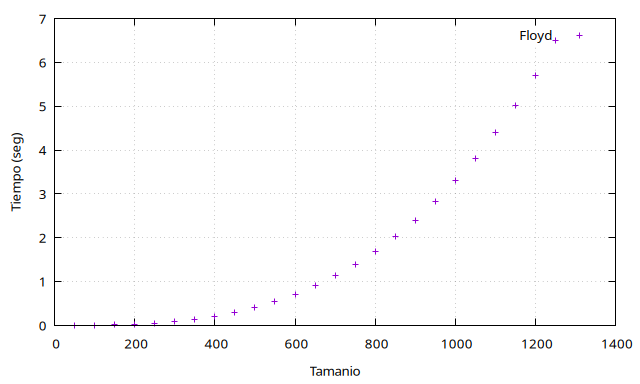
\includegraphics[width=0.8\linewidth]{images/Floyd/floyd_puntos.png}
        \caption{Tiempo de ejecución del algoritmo de Floyd según el tamaño en PC Irina.}
        \label{fig:floyd_puntos}
    \end{figure}

    Habiendo estudiado el análisis teórico, sabemos que el algoritmo es de eficiencia $O(n^3)$. Buscamos una regresión según la función $f(x) = ax^3$, donde $a$ es una constante que vamos a calcular mediante los datos empíricos medidos. Usamos \verb|gnuplot| para calcular la regresión y para representarlo en la Figura \ref{fig:floyd_regresion}. El ajuste que nos da la regresión es:
    $$ax^3 \qquad \text{con} \qquad
         a = 3.30642 \cdot 10^{-9}$$

    \begin{figure}
        \centering
        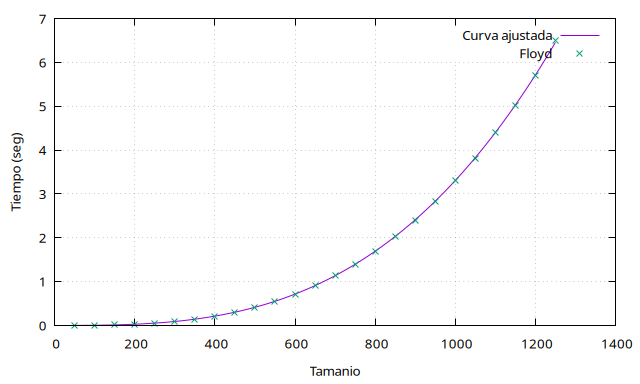
\includegraphics[width=0.8\linewidth]{images/Floyd/floyd.png}
        \caption{Regresión aplicada al algoritmo de Floyd en PC Irina.}
        \label{fig:floyd_regresion}
    \end{figure}

    Tenemos entonces que la función de regresión es:
    \begin{equation*}
        f(x) = 3.30642 \cdot 10^{-9} \cdot x^3
    \end{equation*}
    Además en la gráfica de la Figura \ref{fig:floyd_regresion} podemos observar que se hace un ajuste muy bueno, y los datos que nos ofrece \verb|gnuplot| nos indican que solo han hecho falta 5 iteraciones para llegar a dicho ajuste. De aquí podemos deducir que es un algoritmo bastante estable. 

    \subsubsection{Comparación en distinto hardware}
    Mostramos la Tabla \ref{tab:comp_hardware_floyd} con los tiempos de ejecución en cada uno de los ordenadores del algoritmo de Floyd y una gráfica en la Figura \ref{fig:CompHardwareFloyd} en la que vemos el tiempo de ejecución en cada ordenador.
    \begin{table}
        \centering
        \begin{tabular}{|l|l|l|l|l|l|}
            \hline
            $n$ & José Juan & Arturo & Irina & Lucas & Airam \\
            \hline
            $50$ & $0.000603$ & $0.001159$ & $0.000449805$ & $0.001847$ & $0.00138499$ \\
            $100$ & $0.004542$ & $0.013131$ & $0.00337267$ & $0.012631$ & $0.0110037$ \\
            $150$ & $0.0441$ & $0.026228$ & $0.0115654$ & $0.013884$ & $0.03537$ \\
            $200$ & $0.035143$ & $0.059772$ & $0.0271475$ & $0.02809$ & $0.0852457$ \\
            $250$ & $0.068313$ & $0.095128$ & $0.0536884$ & $0.052543$ & $0.156427$ \\
            $300$ & $0.117504$ & $0.16313$ & $0.091903$ & $0.090714$ & $0.256682$ \\
            $350$ & $0.186478$ & $0.275216$ & $0.143536$ & $0.143473$ & $0.395706$ \\
            $400$ & $0.304537$ & $0.40694$ & $0.214013$ & $0.213136$ & $0.602894$ \\
            $450$ & $0.422511$ & $0.544064$ & $0.304792$ & $0.312363$ & $0.840254$ \\
            $500$ & $0.540751$ & $0.74787$ & $0.415365$ & $0.424881$ & $1.16819$ \\
            $550$ & $0.747692$ & $1.10025$ & $0.552097$ & $0.563973$ & $1.568$ \\
            $600$ & $0.93305$ & $1.29331$ & \underline{$0.714185$} & $0.738205$ & \underline{$2.08373$} \\
            $650$ & $1.18336$ & $1.63547$ & $0.910873$ & $0.927077$ & $2.57425$ \\
            $700$ & $1.47721$ & $2.03938$ & $1.13693$ & $1.16598$ & $3.2336$ \\
            $750$ & $1.81361$ & $2.52209$ & $1.39432$ & $1.41559$ & $4.00494$ \\
            $800$ & $2.20274$ & $3.1811$ & $1.69703$ & $1.74523$ & $4.87717$ \\
            $850$ & $2.64064$ & $3.80557$ & $2.02785$ & $2.08503$ & $5.80996$ \\
            $900$ & $3.13418$ & $4.63116$ & $2.40473$ & $2.4943$ & $6.85551$ \\
            $950$ & $3.68503$ & $5.54908$ & $2.8274$ & $2.90362$ & $8.09525$ \\
            $1000$ & $4.31219$ & $6.63507$ & $3.29641$ & $3.52293$ & $9.50607$ \\
            $1050$ & $4.99056$ & $7.29339$ & $3.81262$ & $3.951$ & $10.8454$ \\
            $1100$ & $5.73665$ & $8.35357$ & $4.40302$ & $4.62134$ & $12.5006$ \\
            $1150$ & $6.45164$ & $9.74663$ & $5.01334$ & $5.25637$ & $14.255$ \\
            $1200$ & $7.42755$ & $10.9512$ & $5.69402$ & $6.01818$ & $16.1939$ \\
            $1250$ & $8.39534$ & $13.209$ & \underline{$6.50325$} & $6.73471$ & \underline{$18.1392$} \\
            \hline
        \end{tabular}
        \caption{Comparación Floyd en distinto hardware.}
        \label{tab:comp_hardware_floyd}
    \end{table}
    \begin{figure}
        \centering
        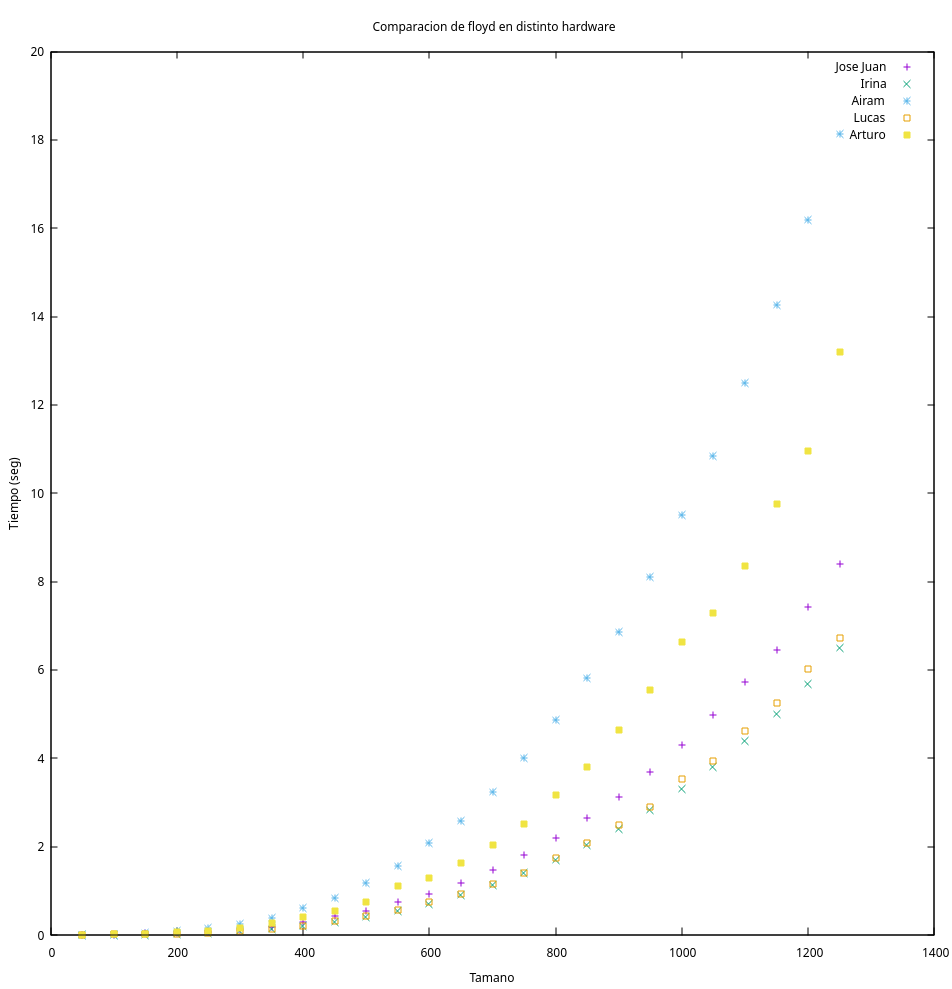
\includegraphics[width=\linewidth]{images/Comparaciones_hardware/Comparacion_hardware_floyd.png}
        \caption{Floyd en todos los PCs.}
        \label{fig:CompHardwareFloyd}
    \end{figure}

    En esta, podemos observar un comportamiento similar a lo que ocurría con la comparativa de algoritmos cuadráticos: para tamaños no muy grandes del problema, como $600$, obtenemos una diferencia en tiempos de ejecución no muy grande, de $2$ segundos entre el hardware con mejor resultados y aquel con peores resultados. Sin embargo, a medida que aumentamos el tamaño del problema, observamos que la pendiente de la gráfica aumenta: observamos un crecimiento moderado en los PCs de Irina, Lucas y José Juan; y un crecimiento grande en los PCs de Arturo y Airam, alcanzando para el último valor de $n$ considerado, $1250$, una diferencia de hasta $11.5$ segundos entre el PC de Irina y el de Airam. Al igual que ocurría en los algoritmos cuadráticos, el hardware influye bastante en los tiempos de ejecución de los algoritmos cúbicos. De hecho, más que para los cuadráticos, ya que aquí observamos una pendiente más pronunciada que en la gráfica de los cuadráticos, ya que un hardware con mejores resultados sostiene mejor el crecimiento de la pendiente, que es mayor en cúbicos que en cuadráticos. 
    
    \subsection{Algoritmos exponenciales}
    \subsubsection{Análisis teórico}
    \textbf{Fibonacci}
    
    El código del algoritmo de Fibonacci se encuentra en el Código fuente \ref{code:fibonacci}.
    
    \begin{listing}
        \begin{minted}[linenos,xleftmargin=3cm]{c++}
int fibo(int n){
    if (n < 2) return 1;
    else return fibo(n-1) + fibo(n-2);
}
        \end{minted}
        \caption{Algoritmo para la sucesión de Fibonacci.}
        \label{code:fibonacci}
    \end{listing}

    El tamaño de nuestro problema es $n$. Supongamos que la función tiene un tiempo de ejecución $T(n)$. Tenemos entonces la siguiente ecuación para la función:
    $$T(n) = \left\{\begin{array}{lcl}
        1 & si & n < 2 \\
        T(n-1) + T(n-2) + 1 & si & n \geq 2
    \end{array} \right.$$

    Aplicamos el método de la ecuación característica. Empezaremos buscando las raíces de la ecuación lineal homogénea. Notando $T(n)=x^n$, tenemos que:
    \begin{equation*}
        x^n - x^{n-1} - x^{n-2} = x^{n-2}(x^2-x-1) = 0
    \end{equation*}

    Por tanto, el polinomio característico asociado a la parte homogénea es:
    \begin{gather*}
        p(x) = x^2-x-1 = \left(x-\left(\frac{1+\sqrt{5}}{2}\right)\right)\cdot \left(x-\left(\frac{1-\sqrt{5}}{2}\right)\right)
    \end{gather*}

    Si ahora tenemos en cuenta la parte no homogénea, tenemos que $1=1^n(n^0)$, por lo que el polinomio característico de la ecuación en diferencias queda:
    \begin{gather*}
         p(x) = \left(x-\left(\frac{1+\sqrt{5}}{2}\right)\right)\cdot \left(x-\left(\frac{1-\sqrt{5}}{2}\right)\right)\cdot (x-1) \implies
    \end{gather*}

    La solución entonces de la Ley de Recurrencia es:
    \begin{equation*}
        T(n)=t_n = c_1 \left(\frac{1+\sqrt{5}}{2}\right)^n + c_2 \left(\frac{1-\sqrt{5}}{2}\right)^n + c_3 \cdot 1^n
    \end{equation*}

    Por la regla del máximo deducimos que es exponencial; es decir:
    \begin{equation*}
        T(n) \in O\left(\left(\frac{1+\sqrt{5}}{2}\right)^n\right)
    \end{equation*}
    
    \textbf{Hanoi}
    
    El código del algoritmo de Hanoi se encuentra en el Código fuente \ref{code:Hanoi}.

        \begin{listing}
        \begin{minted}[linenos,xleftmargin=3cm]{c++}
void hanoi(int M, int i, int j)
{
  if (M > 0)
  {
    hanoi(M - 1, i, 6 - i - j);
    cout << i << " -> " << j << endl;
    hanoi(M - 1, 6 - i - j, j);
  }
}
        \end{minted}
        \caption{Algoritmo resolver el problema Hanoi.}
        \label{code:Hanoi}
    \end{listing}
    
    
    Analizamos el código y vemos que es muy simple, evaluar la condición y
    llevar cada paso a la salida estándar tienen un orden de tiempo constante (aunque en la práctica, bastante duradero debido a la cantidad de llamadas E/S).
    Sin embargo, se hacen dos llamadas recursivas por cada llamada a la función, por lo que tendremos que expresar en términos de una función recurrente el tiempo de ejecución. La función que determina el tiempo que tarda Hanoi en ejecutarse viene dada por:
    $$T(n) = \left\{\begin{array}{lcl}
        2T(n-1) + 1 & si & n \geq 1 \\
        1 & si & n = 0
    \end{array} \right.$$
    Desarrollando de forma recurrente, vemos que:
    \begin{align*}
        T(n) &= 2T(n-1) + 1 = 2(2T(n-2)+1) + 1 
        =\\&= 2^2T(n-2) + 2 + 1 = 2^3 T(n-3) + 4 + 2 + 1=\ldots
        =\\&= 2^kT(n-k) + \sum^{k-1}_{i=0} 2^i = 2^kT(n-k) + 2^k - 1 \qquad \forall k\in \bb{N}, k\geq n
    \end{align*}
    
    Tomamos $k = n$ para tener entonces que:
    $$T(n) = 2^n T(0) + 2^n - 1 = 2 \cdot 2^n - 1$$

    Con esto, concluimos que claramente el algoritmo que resuelve el problema de las torres de Hanoi es $O(2^n)$.
    
    \subsubsection{Análisis empírico e híbrido}
    \textbf{Fibonacci}
    
    Tras ejecutar el algoritmo de Fibonacci para tamaños de $n$ de $2$ a $50$ con saltos de $2$, 
    obtenemos la Tabla \ref{tab:fibonacci_tiempos} que relaciona el tamaño de $n$ con su tiempo de ejecución en segundos. Representamos también los datos en una gráfica en la Figura \ref{fig:fibonacci_puntos} con ayuda de \verb|gnuplot|.
    \begin{table}
        \centering
        \begin{tabular}{|l|l|}
            \hline
            Tamaño de $n$ & Tiempo de ejecución (seg) \\
            \hline
            $2$ & $1.01\cdot 10^{-7}$ \\
            $4$ & $1.6\cdot 10^{-7}$ \\
            $6$ & $2.4\cdot 10^{-7}$ \\
            $8$ & $4.51\cdot 10^{-7}$ \\
            $10$ & $6.81\cdot 10^{-7}$ \\
            $12$ & $1.123\cdot 10^{-6}$ \\
            $14$ & $2.705\cdot 10^{-6}$ \\
            $16$ & $5.801\cdot 10^{-6}$ \\
            $18$ & $1.1943\cdot 10^{-5}$ \\
            $20$ & $3.8093\cdot 10^{-5}$ \\
            $22$ & $8.4522\cdot 10^{-5}$ \\
            $24$ & $0.000195986$ \\
            $26$ & $0.000647991$ \\
            $28$ & $0.00167728$ \\
            $30$ & $0.00351789$ \\
            $32$ & $0.00918415$ \\
            $34$ & $0.0242092$ \\
            $36$ & $0.0640642$ \\
            $38$ & $0.165698$ \\
            $40$ & $0.429828$ \\
            $42$ & $1.13613$ \\
            $44$ & $2.97267$ \\
            $46$ & $7.73283$ \\
            $48$ & $20.164$ \\
            $50$ & $53.4597$ \\
            \hline
        \end{tabular}
        \caption{Tiempos de ejecución para Fibonacci en el ordenador de Irina.}
        \label{tab:fibonacci_tiempos}
    \end{table}
    \begin{figure}
        \centering
        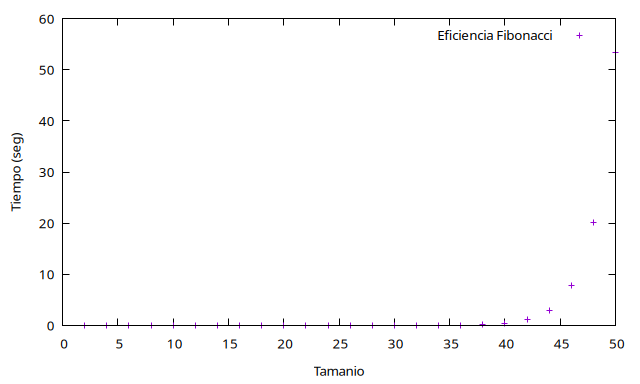
\includegraphics[width=\linewidth]{images/Fibonacci/fibonacci_solopuntos.png}
        \caption{Tiempo de ejecución del Fibonacci según el tamaño en PC Irina.}
        \label{fig:fibonacci_puntos}
    \end{figure}

    Por el análisis teórico del algoritmo, sabemos que la eficiencia del algoritmo es $O\left(\left(\frac{1+\sqrt{5}}{2}\right)^n\right)$, con $\frac{1+\sqrt{5}}{2} \approx 1.618$. Vamos a buscar entonces un ajuste según la función $f(x) = a\cdot 1.618^{b\cdot x}$, donde $a$ y $b$ son constantes que calculamos gracias a los datos empíricos medidos. Usamos \verb|gnuplot| para esta tarea, además de representar la gráfica de la Figura \ref{fig:fibonacci_regresion}. El ajuste que nos da la regresión realizada es el siguiente:
    $$a \cdot 1.618^{b \cdot n} \qquad \text{con} \qquad \left\{\begin{array}{l}
         a = 1.55082 \cdot 10^{-9} \\
         b = 1.00846
    \end{array}\right.$$

    \begin{figure}
        \centering
        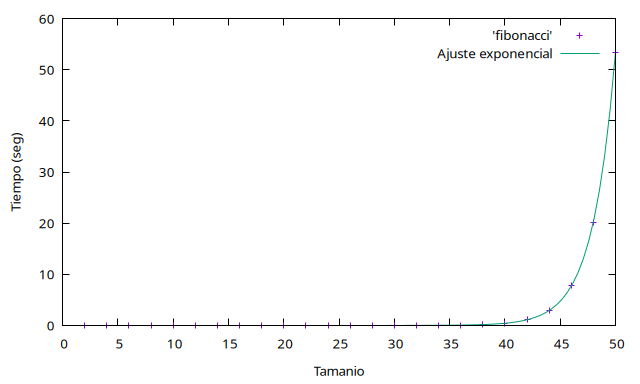
\includegraphics[width=\linewidth]{images/Fibonacci/fibonacci.png}
        \caption{Regresión del algoritmo de Fibonacci en PC Irina.}
        \label{fig:fibonacci_regresion}
    \end{figure}

    Luego nuestra función de regresión es:
    \begin{equation*}
        f(x) = 1.55082\cdot 10^{-9}\cdot 1.618^{1.000846\cdot x}
    \end{equation*}
    Se ve muy claro en la gráfica de la Figura \ref{fig:fibonacci_regresion} el carácter exponencial del algoritmo puesto que hasta $n=40$ no tarda más de un segundo; aunque incluso en esos primeros $40$ valores la escala va creciendo rápido, lo que se puede ver en la Tabla \ref{tab:fibonacci_tiempos}. Pero a partir de $n=42$ se puede ver más fácilmente: $1, 2, 7, 20$ y $53$ segundos aproximadamente. Teniendo en cuenta que en todos son saltos de 2, vemos claramente que sube exponencialmente.\\

    \textbf{Hanoi}
    
    Tras ejecutar el algoritmo de Hanoi para tamaños de $n$ de $3$ a $33$ con saltos de $1$, obtenemos la Tabla \ref{tab:hanoi_tiempos} que relaciona el tamaño de $n$ con su tiempo de ejecución en segundos. Representamos además estos resultados en la gráfica de la Figura \ref{fig:hanoi_puntos} con la ayuda de \verb|gnupot|.
    \begin{table}
        \centering
        \begin{tabular}{|l|l|}
            \hline
            Tamaño de $n$ & Tiempo de ejecución (seg) \\
            \hline
            $3$ & $1.6\cdot 10^{-7}$\\
            $4$ & $2.5\cdot 10^{-7}$\\
            $5$ & $3.5\cdot 10^{-7}$\\
            $6$ & $5.21\cdot 10^{-7}$\\
            $7$ & $2.665\cdot 10^{-6}$\\
            $8$ & $4.308\cdot 10^{-6}$\\
            $9$ & $7.835\cdot 10^{-6}$\\
            $10$ & $1.7313\cdot 10^{-5}$\\
            $11$ & $2.8524\cdot 10^{-5}$\\
            $12$ & $5.6017\cdot 10^{-5}$\\
            $13$ & $0.000111002$\\
            $14$ & $0.00022041$\\
            $15$ & $0.000430572$\\
            $16$ & $0.000877333$\\
            $17$ & $0.00175262$\\
            $18$ & $0.00352908$\\
            $19$ & $0.00703891$\\
            $20$ & $0.0140495$\\
            $21$ & $0.0276141$\\
            $22$ & $0.0559939$\\
            $23$ & $0.0860842$\\
            $24$ & $0.0732093$\\
            $25$ & $0.179872$\\
            $26$ & $0.292778$\\
            $27$ & $0.585756$\\
            $28$ & $1.17102$\\
            $29$ & $2.34124$\\
            $30$ & $4.68704$\\
            $31$ & $9.36798$\\
            $32$ & $18.7341$\\
            $33$ & $37.4663$\\
            \hline
        \end{tabular}
        \caption{Tiempos de ejecución para Hanoi en el ordenador de José Juan.}
        \label{tab:hanoi_tiempos}
    \end{table}
    
    \begin{figure}
        \centering
        \includegraphics[width=0.8\linewidth]{images/Hanoi/hanoi-puntos.png}
        \caption{Tiempo de ejecución de Hanoi según el tamaño en PC José Juan.}
        \label{fig:hanoi_puntos}
    \end{figure}

    El análisis teórico nos dice que se trata de un algoritmo de eficiencia $O(2^n)$. Por tanto, tratamos de buscar una regresión según una función del estilo $a \cdot 2^{n}$ donde $a$ es una constante que buscamos mediante los datos empíricos obtenidos. Usamos \verb|gnuplot| para su regresión y representación gráfica en la Figura \ref{fig:hanoi_regresion}.
    El ajuste que nos da la regresión es:
    $$f(x)=a \cdot 2^{x} \qquad \text{con} \qquad a = 4.38663 \cdot 10^{-9} $$
    
    \begin{figure}
        \centering
        \includegraphics[width=.8\linewidth]{images/Hanoi/hanoi-regresion.png}
        \caption{Regresión aplicada al algoritmo de Hanoi en PC José Juan.}
        \label{fig:hanoi_regresion}
    \end{figure}
 
    \subsubsection{Comparación de algoritmos exponenciales}

    Es el momento de realizar la comparación entre los distintos algoritmos exponenciales que hemos visto, Hanoi y Fibonacci. Para ello hemos construido una gráfica donde se aprecia la diferencia entre los distintos ajustes de estos algoritmos. Con ello conseguiremos determinar cuál de ambos algoritmos es más eficiente. Los datos de ambos algoritmos se encuentran recopilados en la Tabla \ref{tab:fibonacci_hanoi} que podemos observar gráficamente en la Figura \ref{fig:fibo_hanoi_puntos}. En este caso se ha realizado en el caso más sencillo, es decir, para el tipo \verb|int|.
    \begin{table}
        \centering
        \begin{tabular}{|c|c||c|c|}
            \hline
            $n$ & Fibonacci & $n$ & Hanoi \\
            \hline
            $2$  & $3.9\cdot 10^{-7}$ & $3$  & $5.99\cdot 10^{-7}$ \\
            $4$  & $5.46\cdot 10^{-7}$ & $4$  & $7.98\cdot 10^{-7}$ \\
            $6$  & $9.51\cdot 10^{-7}$ & $5$  & $1.5\cdot 10^{-6}$ \\
            $8$  & $1.275\cdot 10^{-6}$ & $6$  & $1.616\cdot 10^{-6}$ \\
            $10$ & $3.009\cdot 10^{-6}$ & $7$  & $2.671\cdot 10^{-6}$ \\
            $12$ & $3.941\cdot 10^{-6}$ & $8$  & $3.962\cdot 10^{-6}$ \\
            $14$ & $8.844\cdot 10^{-6}$ & $9$  & $7.972\cdot 10^{-6}$ \\
            $16$ & $2.1815\cdot 10^{-5}$ & $10$ & $1.3234\cdot 10^{-5}$ \\
            $18$ & $5.3475\cdot 10^{-5}$ & $11$ & $2.6074\cdot 10^{-5}$ \\
            $20$ & $0.000136905$ & $12$ & $4.9961\cdot 10^{-5}$ \\
            $22$ & $0.000367394$ & $13$ & $9.9579\cdot 10^{-5}$ \\
            $24$ & $0.000940697$ & $14$ & $0.000197581$ \\
            $26$ & $0.00252106$ & $15$ & $0.000392722$ \\
            $28$ & $0.00625692$ & $16$ & $0.000835642$ \\
            $30$ & $0.0126508$ & $17$ & $0.00165139$ \\
            $32$ & $0.0178029$ & $18$ & $0.00314614$ \\
            $34$ & $0.0323833$ & $19$ & $0.00591598$ \\
            $36$ & $0.0824038$ & $20$ & $0.00642067$ \\
            $38$ & $0.216716$ & $21$ & $0.010082$ \\
            $40$ & $0.571192$ & $22$ & $0.0166809$ \\
            $42$ & $1.49193$ & $23$ & $0.0280198$ \\
            $44$ & $3.96064$ & $24$ & $0.0555396$ \\
            $46$ & $10.3372$ & $25$ & $0.113143$ \\
            $48$ & $27.5995$ & $26$ & $0.225693$ \\
            $50$ & $73.7711$ & $27$ & $0.455376$ \\
            & & $29$ & $1.83801$ \\
            & & $30$ & $3.67708$ \\
            & & $31$ & $7.38961$ \\
            & & $32$ & $15.0929$ \\
            & & $33$ & $30.0923$ \\
            \hline
        \end{tabular}
        \caption{Tabla comparativa de Fibonacci y Hanoi en el PC Lucas.}
        \label{tab:fibonacci_hanoi}
    \end{table}

    %Grafica solo puntos
    \begin{figure}
        \centering
        \includegraphics[width=\linewidth]{images/Comparaciones/fibonacci_hanoi_puntos.png}
        \caption{Gráfica comparativa de Fibonacci y Hanoi, ambos en el PC de Lucas.}
        \label{fig:fibo_hanoi_puntos}
    \end{figure}

    Antes de comentar nada sobre la gráfica de la Figura \ref{fig:fibo_hanoi_puntos}, es importante aclarar que no es demasiado relevante el resultado expuesto en ella. Esto es así a causa de que el orden de eficiencia de cada uno de los algoritmos, pese a ser ambos de orden exponencial, tienen base distinta ocasionando así que cada paso dado en el tamaño aumente de forma exponencial la diferencia entre los tiempos de ejecución de estos algoritmos.  Además, cabe resaltar que cada algoritmo ha tenido un número de datos tope; en el caso del algoritmo de Hanoi como máximo se tomaron 33 datos y en el caso de Fibonacci se tomaron 50 datos.

    No obstante, es posible deducir cuál de ellos tiene mejor comportamiento. Claramente, si miramos en pocos datos ambos algoritmos tienen un comportamiento prácticamente idéntico, con tiempos prácticamente nulos o inapreciables en la gráfica. A medida que nos alejamos del origen, podemos comprobar que el tiempo de ejecución del algoritmo de Hanoi se dispara a partir de los 30 datos; en contraste con el algoritmo de Fibonacci que sigue con datos inapreciables y no es hasta los 40 datos cuando el tiempo de ejecución comienza a realizar una subida exponencial. 

    Por tanto, pese a que no haya el mismo número de datos, podemos concluir que el algoritmo de Fibonacci es más eficiente que el algoritmo de Hanoi. Esto es claro, pues la base de la función exponencial es distinta en cada caso, siendo la de Fibonacci más pequeña.
    
    
    \subsubsection{Comparación en distinto hardware}
    Como algoritmo exponencial para ejecutarse en todos los ordenadores hemos elegido el algoritmo de Fibonacci. Mostramos ahora la Tabla \ref{tab:comp_hardware_fibonacci} con los tiempos de ejecución en cada uno de los ordenadores y una gráfica en la Figura \ref{fig:CompHardwareFibonacci} en la que vemos el tiempo de ejecución en cada ordenador. La gráfica de los tiempos por sí sola apenas puede apreciarse bien, por lo que decidimos incluir en esta las curvas de regresión; a diferencia de lo hecho en otras ocasiones. Observando la tabla, vemos que para tamaños del problema suficientemente grandes, (por ejemplo, a partir de $n = 44$) obtenemos una disparidad considerable en cuanto a tiempos de ejecución en distinto hardware: diferencias de hasta 7 segundos. Conforme aumentamos el tamaño, esta diferencia se dispara debido a la naturaleza de las funciones exponenciales, llegando hasta una diferencia de 144 segundos para $n=50$ entre los ordenadores de Irina y Airam. Como podemos observar, en el caso de los algoritmos exponenciales, la bondad del hardware es aún más importante, ya que este retrasa el ``estallido'' de los datos a partir de uno en adelante (observemos que en el PC de Irina hay una diferencia considerable entre los datos a partir de $n=46$, mientras que esta diferencia se aprecia en el PC de Airam a partir de $n=42$).
    
    \begin{table}
        \centering
        \begin{tabular}{|l|l|l|l|l|l|}
            \hline
            $n$ & José Juan & Arturo & Irina & Lucas & Airam \\
            \hline
            $2$ & $3.51\cdot 10^{-7}$ & $1.75\cdot 10^{-7}$ & $1.01\cdot 10^{-7}$ & $3.9\cdot 10^{-7}$ & $2.94\cdot 10^{-7}$ \\
            $4$ & $1.4\cdot 10^{-7}$ & $3.59\cdot 10^{-7}$ & $1.6\cdot 10^{-7}$ & $5.46\cdot 10^{-7}$ & $4.55\cdot 10^{-7}$ \\
            $6$ & $2.2\cdot 10^{-7}$ & $3.42\cdot 10^{-7}$ & $2.4\cdot 10^{-7}$ & $9.51\cdot 10^{-7}$ & $6.49\cdot 10^{-7}$ \\
            $8$ & $3.81\cdot 10^{-7}$ & $7.58\cdot 10^{-7}$ & $4.51\cdot 10^{-7}$ & $1.275\cdot 10^{-6}$ & $1.139\cdot 10^{-6}$ \\
            $10$ & $6.81\cdot 10^{-7}$ & $1.309\cdot 10^{-6}$ & $6.81\cdot 10^{-7}$ & $3.009\cdot 10^{-6}$ & $2.302\cdot 10^{-6}$ \\
            $12$ & $1.423\cdot 10^{-6}$ & $2.232\cdot 10^{-6}$ & $1.123\cdot 10^{-6}$ & $3.941\cdot 10^{-6}$ & $3.573\cdot 10^{-6}$ \\
            $14$ & $9.337\cdot 10^{-6}$ & $1.4181\cdot 10^{-5}$ & $2.705\cdot 10^{-6}$ & $8.844\cdot 10^{-6}$ & $7.947\cdot 10^{-6}$ \\
            $16$ & $6.682\cdot 10^{-6}$ & $1.0605\cdot 10^{-5}$ & $5.801\cdot 10^{-6}$ & $2.1815\cdot 10^{-5}$ & $2.0002\cdot 10^{-5}$ \\
            $18$ & $1.8245\cdot 10^{-5}$ & $2.6339\cdot 10^{-5}$ & $1.1943\cdot 10^{-5}$ & $5.3475\cdot 10^{-5}$ & $4.9157\cdot 10^{-5}$ \\
            $20$ & $4.6427\cdot 10^{-5}$ & $8.7014\cdot 10^{-5}$ & $3.8093\cdot 10^{-5}$ & $0.000136905$ & $0.000125821$ \\
            $22$ & $0.000123191$ & $0.000210895$ & $8.4522\cdot 10^{-5}$ & $0.000367394$ & $0.000328948$ \\
            $24$ & $0.000297878$ & $0.00194832$ & $0.000195986$ & $0.000940697$ & $0.00087767$ \\
            $26$ & $0.000764572$ & $0.00122205$ & $0.000647991$ & $0.00252106$ & $0.0022649$ \\
            $28$ & $0.00199871$ & $0.00337777$ & $0.00167728$ & $0.00625692$ & $0.0059107$ \\
            $30$ & $0.00547652$ & $0.00864883$ & $0.00351789$ & $0.0126508$ & $0.0141414$ \\
            $32$ & $0.0142995$ & $0.0213254$ & $0.00918415$ & $0.0178029$ & $0.0372582$ \\
            $34$ & $0.0371424$ & $0.0549702$ & $0.0242092$ & $0.0323833$ & $0.102112$ \\
            $36$ & $0.0980092$ & $0.138956$ & $0.0640642$ & $0.0824038$ & $0.243725$ \\
            $38$ & $0.247195$ & $0.397855$ & $0.165698$ & $0.216716$ & $0.63263$ \\
            $40$ & $0.646761$ & $0.980171$ & $0.429828$ & $0.571192$ & $1.59775$ \\
            $42$ & $1.7614$ & $2.47504$ & $1.13613$ & $1.49193$ & $4.24822$ \\
            $44$ & $4.58162$ & $6.62743$ & \underline{$2.97267$} & $3.96064$ & \underline{$10.9739$} \\
            $46$ & $11.6635$ & $18.0981$ & $7.73283$ & $10.3372$ & $28.7114$ \\
            $48$ & $30.3569$ & $45.845$ & $20.164$ & $27.5995$ & $76.4746$ \\
            $50$ & $80.9576$ & $120.518$ & $53.4597$ & $73.7711$ & $197.166$ \\
            \hline
        \end{tabular}
        \caption{Comparación del algoritmo de Fibonacci en distinto hardware.}
        \label{tab:comp_hardware_fibonacci}
    \end{table}
    \begin{figure}
        \centering
        \includegraphics[width=\linewidth]{images/Comparaciones_hardware/Comparacion_hardware_fibonacci.png}
        \caption{Comparación del algoritmo de Fibonacci en todos los PCs.}
        \label{fig:CompHardwareFibonacci}
    \end{figure}

    \section{Conclusiones}
    %Enumerar y describir las principales conclusiones derivadas del trabajo realizado en esta práctica.
    
    Las conclusiones alcanzadas en el presente informe son varias y de diversa índole. Grosso modo, hemos comprendido de forma real lo que implica la notación $O$, ya que estamos muy acostumbrados a asignar a cada algoritmo un orden de eficiencia sin saber lo que esto implica.

    Como primera gran conclusión, hemos visto que aun siendo dos algoritmos del mismo orden, no necesariamente implica que sean ``igual de buenos'', debido a constantes. Como hemos señalado en la sección correspondiente, aun siendo tanto el algoritmo de ordenación mediante Inserción como Burbuja ambos cuadráticos; el de Inserción es mucho más eficiente, no habiendo motivos aparentes por los que elegir el algoritmo de Burbuja en ningún caso.

    Otra conclusión que hemos obtenido de este estudio es la importancia de entender la diferencia entre el caso peor, el caso promedio, y el caso óptimo. En el caso del Quicksort, por ejemplo, aun siendo de orden $O(n^2)$, cuadrático en el peor caso, en el caso promedio se comporta como un algoritmo lineal-logarítmico. Por ello, pese a ser de orden cuadrático, no se suele englobar con los algoritmos no recursivos como el de Inserción; sino con los recursivos como el Mergesort.

    Asimismo, también nos hemos dado cuenta de la importancia del estudio teórico de los algoritmos previamente a su implementación, ya que si estos no son buenos no va a tener sentido implementarlos, pues van a ser inútiles al tardar estos demasiado. Para tamaños del problema grandes, esto será esencial para poder llegar a cualquier resultado.

    Por otra parte, hemos visto como también afectan los tipos de datos empleados para un problema, siendo por ejemplo el \verb|string| un tipo de dato cuya ordenación es mucho más costosa dada la complejidad que supone hacer por ejemplo el \verb|swap| de dos cadenas. Esto puede causar un gran deterioro en el paradigma de programación orientada a objetos (por ejemplo), al tener que manipular objetos con numerosos atributos. 

    Además, hemos concluido que el hardware empleado en la ejecución de los algoritmos juega un gran papel en sus tiempos de ejecución, sobre todo en el caso de los algoritmos de peor orden (los menos eficientes). Junto con tamaños de problema grandes y algoritmos inadecuados, podemos llegar a obtener tiempos no deseados, sobre todo si no se dispone de un buen hardware. Por tanto, ante problemas que puedan ser escalables, debemos buscar siempre una solución óptima que retarde el crecimiento de tiempos de ejecución.

    Otra cuestión que hemos podido comprobar es la diferencia en cuanto a la base de un orden de eficiencia exponencial: ante una pequeña perturbación en la base de este (como ocurre con Fibonacci y Hanoi) obtenemos una diferencia notoria en cuanto a tiempos de ejecución. Por tanto, no tiene sentido comparar dos algoritmos de ese estilo, pues admiten escalas de datos muy diferentes. 

    En general, nos ha sido de gran ayuda porque nos ha ayudado a plasmar los conocimientos teóricos que teníamos en mente de una forma empírica, aprendiendo de ellos.
\end{document}